% Options for packages loaded elsewhere
\PassOptionsToPackage{unicode}{hyperref}
\PassOptionsToPackage{hyphens}{url}
%
\documentclass[
]{memoir}
\usepackage{amsmath,amssymb}
\usepackage{lmodern}
\usepackage{iftex}
\ifPDFTeX
  \usepackage[T1]{fontenc}
  \usepackage[utf8]{inputenc}
  \usepackage{textcomp} % provide euro and other symbols
\else % if luatex or xetex
  \usepackage{unicode-math}
  \defaultfontfeatures{Scale=MatchLowercase}
  \defaultfontfeatures[\rmfamily]{Ligatures=TeX,Scale=1}
  \setmainfont[]{Roboto}
  \setsansfont[]{Clancy}
  \setmonofont[]{Roboto Mono}
\fi
% Use upquote if available, for straight quotes in verbatim environments
\IfFileExists{upquote.sty}{\usepackage{upquote}}{}
\IfFileExists{microtype.sty}{% use microtype if available
  \usepackage[]{microtype}
  \UseMicrotypeSet[protrusion]{basicmath} % disable protrusion for tt fonts
}{}
\makeatletter
\@ifundefined{KOMAClassName}{% if non-KOMA class
  \IfFileExists{parskip.sty}{%
    \usepackage{parskip}
  }{% else
    \setlength{\parindent}{0pt}
    \setlength{\parskip}{6pt plus 2pt minus 1pt}}
}{% if KOMA class
  \KOMAoptions{parskip=half}}
\makeatother
\usepackage{xcolor}
\IfFileExists{xurl.sty}{\usepackage{xurl}}{} % add URL line breaks if available
\IfFileExists{bookmark.sty}{\usepackage{bookmark}}{\usepackage{hyperref}}
\hypersetup{
  pdftitle={PHCM9795 Foundations of Biostatistics},
  pdfauthor={Course notes},
  hidelinks,
  pdfcreator={LaTeX via pandoc}}
\urlstyle{same} % disable monospaced font for URLs
\usepackage{color}
\usepackage{fancyvrb}
\newcommand{\VerbBar}{|}
\newcommand{\VERB}{\Verb[commandchars=\\\{\}]}
\DefineVerbatimEnvironment{Highlighting}{Verbatim}{commandchars=\\\{\}}
% Add ',fontsize=\small' for more characters per line
\usepackage{framed}
\definecolor{shadecolor}{RGB}{248,248,248}
\newenvironment{Shaded}{\begin{snugshade}}{\end{snugshade}}
\newcommand{\AlertTok}[1]{\textcolor[rgb]{0.94,0.16,0.16}{#1}}
\newcommand{\AnnotationTok}[1]{\textcolor[rgb]{0.56,0.35,0.01}{\textbf{\textit{#1}}}}
\newcommand{\AttributeTok}[1]{\textcolor[rgb]{0.77,0.63,0.00}{#1}}
\newcommand{\BaseNTok}[1]{\textcolor[rgb]{0.00,0.00,0.81}{#1}}
\newcommand{\BuiltInTok}[1]{#1}
\newcommand{\CharTok}[1]{\textcolor[rgb]{0.31,0.60,0.02}{#1}}
\newcommand{\CommentTok}[1]{\textcolor[rgb]{0.56,0.35,0.01}{\textit{#1}}}
\newcommand{\CommentVarTok}[1]{\textcolor[rgb]{0.56,0.35,0.01}{\textbf{\textit{#1}}}}
\newcommand{\ConstantTok}[1]{\textcolor[rgb]{0.00,0.00,0.00}{#1}}
\newcommand{\ControlFlowTok}[1]{\textcolor[rgb]{0.13,0.29,0.53}{\textbf{#1}}}
\newcommand{\DataTypeTok}[1]{\textcolor[rgb]{0.13,0.29,0.53}{#1}}
\newcommand{\DecValTok}[1]{\textcolor[rgb]{0.00,0.00,0.81}{#1}}
\newcommand{\DocumentationTok}[1]{\textcolor[rgb]{0.56,0.35,0.01}{\textbf{\textit{#1}}}}
\newcommand{\ErrorTok}[1]{\textcolor[rgb]{0.64,0.00,0.00}{\textbf{#1}}}
\newcommand{\ExtensionTok}[1]{#1}
\newcommand{\FloatTok}[1]{\textcolor[rgb]{0.00,0.00,0.81}{#1}}
\newcommand{\FunctionTok}[1]{\textcolor[rgb]{0.00,0.00,0.00}{#1}}
\newcommand{\ImportTok}[1]{#1}
\newcommand{\InformationTok}[1]{\textcolor[rgb]{0.56,0.35,0.01}{\textbf{\textit{#1}}}}
\newcommand{\KeywordTok}[1]{\textcolor[rgb]{0.13,0.29,0.53}{\textbf{#1}}}
\newcommand{\NormalTok}[1]{#1}
\newcommand{\OperatorTok}[1]{\textcolor[rgb]{0.81,0.36,0.00}{\textbf{#1}}}
\newcommand{\OtherTok}[1]{\textcolor[rgb]{0.56,0.35,0.01}{#1}}
\newcommand{\PreprocessorTok}[1]{\textcolor[rgb]{0.56,0.35,0.01}{\textit{#1}}}
\newcommand{\RegionMarkerTok}[1]{#1}
\newcommand{\SpecialCharTok}[1]{\textcolor[rgb]{0.00,0.00,0.00}{#1}}
\newcommand{\SpecialStringTok}[1]{\textcolor[rgb]{0.31,0.60,0.02}{#1}}
\newcommand{\StringTok}[1]{\textcolor[rgb]{0.31,0.60,0.02}{#1}}
\newcommand{\VariableTok}[1]{\textcolor[rgb]{0.00,0.00,0.00}{#1}}
\newcommand{\VerbatimStringTok}[1]{\textcolor[rgb]{0.31,0.60,0.02}{#1}}
\newcommand{\WarningTok}[1]{\textcolor[rgb]{0.56,0.35,0.01}{\textbf{\textit{#1}}}}
\usepackage{longtable,booktabs,array}
\usepackage{calc} % for calculating minipage widths
% Correct order of tables after \paragraph or \subparagraph
\usepackage{etoolbox}
\makeatletter
\patchcmd\longtable{\par}{\if@noskipsec\mbox{}\fi\par}{}{}
\makeatother
% Allow footnotes in longtable head/foot
\IfFileExists{footnotehyper.sty}{\usepackage{footnotehyper}}{\usepackage{footnote}}
\makesavenoteenv{longtable}
\usepackage{graphicx}
\makeatletter
\def\maxwidth{\ifdim\Gin@nat@width>\linewidth\linewidth\else\Gin@nat@width\fi}
\def\maxheight{\ifdim\Gin@nat@height>\textheight\textheight\else\Gin@nat@height\fi}
\makeatother
% Scale images if necessary, so that they will not overflow the page
% margins by default, and it is still possible to overwrite the defaults
% using explicit options in \includegraphics[width, height, ...]{}
\setkeys{Gin}{width=\maxwidth,height=\maxheight,keepaspectratio}
% Set default figure placement to htbp
\makeatletter
\def\fps@figure{htbp}
\makeatother
\setlength{\emergencystretch}{3em} % prevent overfull lines
\providecommand{\tightlist}{%
  \setlength{\itemsep}{0pt}\setlength{\parskip}{0pt}}
\setcounter{secnumdepth}{5}
\usepackage{booktabs}
\usepackage{float}

\floatstyle{boxed}
\newfloat{program}{thp}{lop}
\floatname{program}{Output}

\renewcommand{\chaptername}{Module}
\renewcommand*{\chapnamefont}{\normalfont\HUGE\bfseries\sffamily}
\renewcommand*{\chapnumfont}{\normalfont\HUGE\bfseries\sffamily}
\renewcommand*{\chaptitlefont}{\normalfont\HUGE\bfseries\sffamily}

\setsecheadstyle{\sffamily}% Set \section style
\setsubsecheadstyle{\sffamily}% Set \subsection style
\setsubsubsecheadstyle{\sffamily}% Set \subsubsection style

\setlrmarginsandblock{3.5cm}{2.5cm}{*}
\setulmarginsandblock{2.5cm}{*}{1}
\checkandfixthelayout 
\usepackage{array}
\usepackage{caption}
\usepackage{graphicx}
\usepackage{siunitx}
\usepackage[normalem]{ulem}
\usepackage{colortbl}
\usepackage{multirow}
\usepackage{hhline}
\usepackage{calc}
\usepackage{tabularx}
\usepackage{threeparttable}
\usepackage{wrapfig}
\usepackage{adjustbox}
\usepackage{hyperref}
\ifLuaTeX
  \usepackage{selnolig}  % disable illegal ligatures
\fi
\usepackage[]{natbib}
\bibliographystyle{plainnat}

\title{PHCM9795 Foundations of Biostatistics}
\author{Course notes}
\date{Term 2, 2022}

\begin{document}
\maketitle

{
\setcounter{tocdepth}{1}
\tableofcontents
}
\hypertarget{introduction-to-statistics-and-presenting-data}{%
\chapter{Introduction to statistics and presenting data}\label{introduction-to-statistics-and-presenting-data}}

\hypertarget{learning-objectives}{%
\section*{Learning objectives}\label{learning-objectives}}
\addcontentsline{toc}{section}{Learning objectives}

By the end of this module, you will be able to:

\begin{itemize}
\tightlist
\item
  Define the term statistics;
\item
  Describe and identify the underpinning concepts of descriptive and inferential statistics;
\item
  Distinguish between different types of variables (i.e.~quantitative -- discrete and continuous; and qualitative -- ordinal and nominal);
\item
  Construct appropriate frequency tables from raw data;
\item
  Compute summary statistics to describe the centre and spread of data;
\item
  Describe the (centre and spread of the) data using appropriate graphs (histogram and box plot);
\item
  Present and interpret graphical summaries of variables using a variety of graphs (bar charts, line-graphs, histograms, boxplots, pie charts and others).
\end{itemize}

\hypertarget{readings}{%
\section*{Readings}\label{readings}}
\addcontentsline{toc}{section}{Readings}

\citep{kirkwood_sterne01}; Chapters 2 and 3.

\citep{bland15}; Chapter 4.

\citep{acock10}; Chapter 5.

\hypertarget{an-introduction-to-statistics}{%
\section{An introduction to statistics}\label{an-introduction-to-statistics}}

\hypertarget{module-1-learning-activities}{%
\chapter*{Module 1: Learning Activities}\label{module-1-learning-activities}}
\addcontentsline{toc}{chapter}{Module 1: Learning Activities}

\hypertarget{activity-1.1}{%
\subsection*{Activity 1.1}\label{activity-1.1}}
\addcontentsline{toc}{subsection}{Activity 1.1}

25 participants were enrolled in a 3-week weight loss programme. The following data present the weight loss (in grams) of the participants.

 
  \providecommand{\huxb}[2]{\arrayrulecolor[RGB]{#1}\global\arrayrulewidth=#2pt}
  \providecommand{\huxvb}[2]{\color[RGB]{#1}\vrule width #2pt}
  \providecommand{\huxtpad}[1]{\rule{0pt}{#1}}
  \providecommand{\huxbpad}[1]{\rule[-#1]{0pt}{#1}}

\begin{table}[ht]
\begin{centerbox}
\begin{threeparttable}
\captionsetup{justification=centering,singlelinecheck=off}
\caption{\label{tab:act-1-1} Weight loss (g) for 25 participants}
 \setlength{\tabcolsep}{0pt}
\begin{tabularx}{0.8\textwidth}{p{0.16\textwidth} p{0.16\textwidth} p{0.16\textwidth} p{0.16\textwidth} p{0.16\textwidth}}


\hhline{>{\huxb{0, 0, 0}{0.4}}->{\huxb{0, 0, 0}{0.4}}->{\huxb{0, 0, 0}{0.4}}->{\huxb{0, 0, 0}{0.4}}->{\huxb{0, 0, 0}{0.4}}-}
\arrayrulecolor{black}

\multicolumn{1}{!{\huxvb{0, 0, 0}{0}}p{0.16\textwidth}!{\huxvb{0, 0, 0}{0}}}{\hspace{0pt}\parbox[b]{0.16\textwidth-0pt-6pt}{\huxtpad{6pt + 1em}\raggedleft 255\huxbpad{6pt}}} &
\multicolumn{1}{p{0.16\textwidth}!{\huxvb{0, 0, 0}{0}}}{\hspace{6pt}\parbox[b]{0.16\textwidth-6pt-6pt}{\huxtpad{6pt + 1em}\raggedleft 198\huxbpad{6pt}}} &
\multicolumn{1}{p{0.16\textwidth}!{\huxvb{0, 0, 0}{0}}}{\hspace{6pt}\parbox[b]{0.16\textwidth-6pt-6pt}{\huxtpad{6pt + 1em}\raggedleft 283\huxbpad{6pt}}} &
\multicolumn{1}{p{0.16\textwidth}!{\huxvb{0, 0, 0}{0}}}{\hspace{6pt}\parbox[b]{0.16\textwidth-6pt-6pt}{\huxtpad{6pt + 1em}\raggedleft 312\huxbpad{6pt}}} &
\multicolumn{1}{p{0.16\textwidth}!{\huxvb{0, 0, 0}{0}}}{\hspace{6pt}\parbox[b]{0.16\textwidth-6pt-0pt}{\huxtpad{6pt + 1em}\raggedleft 283\huxbpad{6pt}}} \tabularnewline[-0.5pt]


\hhline{}
\arrayrulecolor{black}

\multicolumn{1}{!{\huxvb{0, 0, 0}{0}}p{0.16\textwidth}!{\huxvb{0, 0, 0}{0}}}{\hspace{0pt}\parbox[b]{0.16\textwidth-0pt-6pt}{\huxtpad{6pt + 1em}\raggedleft 57\huxbpad{6pt}}} &
\multicolumn{1}{p{0.16\textwidth}!{\huxvb{0, 0, 0}{0}}}{\hspace{6pt}\parbox[b]{0.16\textwidth-6pt-6pt}{\huxtpad{6pt + 1em}\raggedleft 85\huxbpad{6pt}}} &
\multicolumn{1}{p{0.16\textwidth}!{\huxvb{0, 0, 0}{0}}}{\hspace{6pt}\parbox[b]{0.16\textwidth-6pt-6pt}{\huxtpad{6pt + 1em}\raggedleft 312\huxbpad{6pt}}} &
\multicolumn{1}{p{0.16\textwidth}!{\huxvb{0, 0, 0}{0}}}{\hspace{6pt}\parbox[b]{0.16\textwidth-6pt-6pt}{\huxtpad{6pt + 1em}\raggedleft 142\huxbpad{6pt}}} &
\multicolumn{1}{p{0.16\textwidth}!{\huxvb{0, 0, 0}{0}}}{\hspace{6pt}\parbox[b]{0.16\textwidth-6pt-0pt}{\huxtpad{6pt + 1em}\raggedleft 113\huxbpad{6pt}}} \tabularnewline[-0.5pt]


\hhline{}
\arrayrulecolor{black}

\multicolumn{1}{!{\huxvb{0, 0, 0}{0}}p{0.16\textwidth}!{\huxvb{0, 0, 0}{0}}}{\hspace{0pt}\parbox[b]{0.16\textwidth-0pt-6pt}{\huxtpad{6pt + 1em}\raggedleft 227\huxbpad{6pt}}} &
\multicolumn{1}{p{0.16\textwidth}!{\huxvb{0, 0, 0}{0}}}{\hspace{6pt}\parbox[b]{0.16\textwidth-6pt-6pt}{\huxtpad{6pt + 1em}\raggedleft 283\huxbpad{6pt}}} &
\multicolumn{1}{p{0.16\textwidth}!{\huxvb{0, 0, 0}{0}}}{\hspace{6pt}\parbox[b]{0.16\textwidth-6pt-6pt}{\huxtpad{6pt + 1em}\raggedleft 255\huxbpad{6pt}}} &
\multicolumn{1}{p{0.16\textwidth}!{\huxvb{0, 0, 0}{0}}}{\hspace{6pt}\parbox[b]{0.16\textwidth-6pt-6pt}{\huxtpad{6pt + 1em}\raggedleft 340\huxbpad{6pt}}} &
\multicolumn{1}{p{0.16\textwidth}!{\huxvb{0, 0, 0}{0}}}{\hspace{6pt}\parbox[b]{0.16\textwidth-6pt-0pt}{\huxtpad{6pt + 1em}\raggedleft 142\huxbpad{6pt}}} \tabularnewline[-0.5pt]


\hhline{}
\arrayrulecolor{black}

\multicolumn{1}{!{\huxvb{0, 0, 0}{0}}p{0.16\textwidth}!{\huxvb{0, 0, 0}{0}}}{\hspace{0pt}\parbox[b]{0.16\textwidth-0pt-6pt}{\huxtpad{6pt + 1em}\raggedleft 113\huxbpad{6pt}}} &
\multicolumn{1}{p{0.16\textwidth}!{\huxvb{0, 0, 0}{0}}}{\hspace{6pt}\parbox[b]{0.16\textwidth-6pt-6pt}{\huxtpad{6pt + 1em}\raggedleft 312\huxbpad{6pt}}} &
\multicolumn{1}{p{0.16\textwidth}!{\huxvb{0, 0, 0}{0}}}{\hspace{6pt}\parbox[b]{0.16\textwidth-6pt-6pt}{\huxtpad{6pt + 1em}\raggedleft 227\huxbpad{6pt}}} &
\multicolumn{1}{p{0.16\textwidth}!{\huxvb{0, 0, 0}{0}}}{\hspace{6pt}\parbox[b]{0.16\textwidth-6pt-6pt}{\huxtpad{6pt + 1em}\raggedleft 85\huxbpad{6pt}}} &
\multicolumn{1}{p{0.16\textwidth}!{\huxvb{0, 0, 0}{0}}}{\hspace{6pt}\parbox[b]{0.16\textwidth-6pt-0pt}{\huxtpad{6pt + 1em}\raggedleft 170\huxbpad{6pt}}} \tabularnewline[-0.5pt]


\hhline{}
\arrayrulecolor{black}

\multicolumn{1}{!{\huxvb{0, 0, 0}{0}}p{0.16\textwidth}!{\huxvb{0, 0, 0}{0}}}{\hspace{0pt}\parbox[b]{0.16\textwidth-0pt-6pt}{\huxtpad{6pt + 1em}\raggedleft 255\huxbpad{6pt}}} &
\multicolumn{1}{p{0.16\textwidth}!{\huxvb{0, 0, 0}{0}}}{\hspace{6pt}\parbox[b]{0.16\textwidth-6pt-6pt}{\huxtpad{6pt + 1em}\raggedleft 198\huxbpad{6pt}}} &
\multicolumn{1}{p{0.16\textwidth}!{\huxvb{0, 0, 0}{0}}}{\hspace{6pt}\parbox[b]{0.16\textwidth-6pt-6pt}{\huxtpad{6pt + 1em}\raggedleft 113\huxbpad{6pt}}} &
\multicolumn{1}{p{0.16\textwidth}!{\huxvb{0, 0, 0}{0}}}{\hspace{6pt}\parbox[b]{0.16\textwidth-6pt-6pt}{\huxtpad{6pt + 1em}\raggedleft 227\huxbpad{6pt}}} &
\multicolumn{1}{p{0.16\textwidth}!{\huxvb{0, 0, 0}{0}}}{\hspace{6pt}\parbox[b]{0.16\textwidth-6pt-0pt}{\huxtpad{6pt + 1em}\raggedleft 255\huxbpad{6pt}}} \tabularnewline[-0.5pt]


\hhline{>{\huxb{0, 0, 0}{0.4}}->{\huxb{0, 0, 0}{0.4}}->{\huxb{0, 0, 0}{0.4}}->{\huxb{0, 0, 0}{0.4}}->{\huxb{0, 0, 0}{0.4}}-}
\arrayrulecolor{black}
\end{tabularx}
\end{threeparttable}\par\end{centerbox}

\end{table}
 

\begin{enumerate}
\def\labelenumi{\alph{enumi})}
\tightlist
\item
  Enter these data into Stata.
\item
  What type of data are these?
\item
  Construct an appropriate graph to display the relative frequency of participants' weight loss. Your graph should start at 50 grams, with weight loss grouped into 50 gram bins. Provide appropriate labels for the axes and give the graph an appropriate title.
\end{enumerate}

\hypertarget{activity-1.2}{%
\subsection*{Activity 1.2}\label{activity-1.2}}
\addcontentsline{toc}{subsection}{Activity 1.2}

Researchers at a maternity hospital in the 1970s conducted a study of low birth weight babies. Low birth weight is classified as a weight of 2,500g or less at birth. Data were collected on age and smoking status of mothers and the birth weight of their babies. The Stata file \texttt{Activity\_S1.2.dta} contains data on the participants in the study. The file is located on Moodle in the Learning Activities section.

Use Stata to create a 2 by 2 table to show the proportions of low birth weight babies born to mothers who smoked during pregnancy and those that did not smoke during pregnancy. Answer the following questions:

\begin{enumerate}
\def\labelenumi{\alph{enumi})}
\tightlist
\item
  What was the total number of mothers who smoked during pregnancy?
\item
  What proportion of mothers who smoked gave birth to low birth weight babies? What proportion of non-smoking mothers gave birth to low birth weight babies?
\item
  Use Stata to construct a stacked bar chart of the data to examine if there a difference in the proportion of babies born with a low birth weight in relation to mother's age? Provide appropriate labels for the axes and give the graph an appropriate title.
\item
  Using your answers to the question a) and b), write a brief conclusion about the relationship of low birth weight and mother's age and smoking status.
\end{enumerate}

\hypertarget{activity-1.3}{%
\subsection*{Activity 1.3}\label{activity-1.3}}
\addcontentsline{toc}{subsection}{Activity 1.3}

Using Stata, estimate the mean, median, mode, standard deviation, range and interquartile range for the data Activity\_S1.3.dta, available on Moodle.

\hypertarget{activity-1.4}{%
\subsection*{Activity 1.4}\label{activity-1.4}}
\addcontentsline{toc}{subsection}{Activity 1.4}

Data of diastolic blood pressure (BP) of a sample of study participants are provided in the dataset Activity\_S1.4.dta. Compute the mean, median, range and SD of diastolic BP.

\hypertarget{activity-1.5}{%
\subsection*{Activity 1.5}\label{activity-1.5}}
\addcontentsline{toc}{subsection}{Activity 1.5}

In a study of 100 participants data were missing for 5 people. The missing data points were coded as `99'. The mean of the data was estimated as 45.0 with a standard deviation of 5.6; the smallest and greatest values are 16 and 65 respectively.

If the researcher analysed the data as if the 99s were real data, would it make the following statistics larger, smaller, or stay the same?

\begin{enumerate}
\def\labelenumi{\alph{enumi})}
\tightlist
\item
  Mean
\item
  Standard Deviation
\item
  Range
\end{enumerate}

\hypertarget{activity-1.6}{%
\subsection*{Activity 1.6}\label{activity-1.6}}
\addcontentsline{toc}{subsection}{Activity 1.6}

Which of the following statements are true? The more dispersed, or spread out, a set of observations are:

\begin{enumerate}
\def\labelenumi{\alph{enumi})}
\tightlist
\item
  The smaller the mean value
\item
  The larger the standard deviation
\item
  The smaller the variance
\end{enumerate}

\hypertarget{activity-1.7}{%
\subsection*{Activity 1.7}\label{activity-1.7}}
\addcontentsline{toc}{subsection}{Activity 1.7}

If the variance for a set of scores is equal to 9, what is the standard deviation?

\hypertarget{probability-and-probability-distributions}{%
\chapter{Probability and probability distributions}\label{probability-and-probability-distributions}}

\hypertarget{learning-objectives-1}{%
\section*{Learning objectives}\label{learning-objectives-1}}
\addcontentsline{toc}{section}{Learning objectives}

By the end of this module you will be able to:

\begin{itemize}
\tightlist
\item
  Describe the concept of probability;
\item
  Describe the characteristics of a binomial distribution and a Normal distribution;
\item
  Compute binomial probabilities using Stata;
\item
  Compute and use Z-scores to obtain probabilities;
\item
  Decide when to use parametric or non-parametric statistical methods;
\item
  Briefly outline other types of distributions.
\end{itemize}

\hypertarget{readings-1}{%
\section*{Readings}\label{readings-1}}
\addcontentsline{toc}{section}{Readings}

\citet{kirkwood_sterne01}; Chapters 5, 14 and 15.

\citet{bland15}; Chapters 6 and 7.

\hypertarget{section}{%
\section{Section}\label{section}}

\hypertarget{module-2-stata-notes}{%
\chapter*{\texorpdfstring{\textbf{Module 2: Stata notes}}{Module 2: Stata notes}}\label{module-2-stata-notes}}
\addcontentsline{toc}{chapter}{\textbf{Module 2: Stata notes}}

\hypertarget{module-2-learning-activities}{%
\chapter*{Module 2: Learning Activities}\label{module-2-learning-activities}}
\addcontentsline{toc}{chapter}{Module 2: Learning Activities}

\hypertarget{activity-2.1}{%
\subsection*{Activity 2.1}\label{activity-2.1}}
\addcontentsline{toc}{subsection}{Activity 2.1}

In a Randomised Controlled Trial, the preference of a new drug was tested against an established drug by giving both drugs to each of 90 people. Assume that the two drugs are equally preferred, that is, the probability that a patient prefers either of the drugs is equal (50\%). Use one of the binomial functions in Stata to compute the probability that 60 or more patients would prefer the new drug. In completing this question, determine:

\begin{enumerate}
\def\labelenumi{\alph{enumi})}
\tightlist
\item
  The number of trials (n)
\item
  The number of successes we are interested in (k)
\item
  The probability of success for each trial (p)
\item
  The form of the Stata function: binomialp, binomial or binomialtail
\item
  The final probability.
\end{enumerate}

\hypertarget{activity-2.2}{%
\subsection*{Activity 2.2}\label{activity-2.2}}
\addcontentsline{toc}{subsection}{Activity 2.2}

A case of Schistosomiasis is identified by the detection of schistosome ova in a faecal sample. In patients with a low level of infection, a field technique of faecal examination has a probability of 0.35 of detecting ova in any one faecal sample. If five samples are routinely examined for each patient, use Stata to compute the probability that a patient with a low level of infection:

\begin{enumerate}
\def\labelenumi{\alph{enumi})}
\tightlist
\item
  Will not be identified?
\item
  Will be identified in two of the samples?
\item
  Will be identified in all the samples?
\item
  Will be identified in at most 3 of the samples?
\end{enumerate}

\hypertarget{activity-2.3}{%
\subsection*{Activity 2.3}\label{activity-2.3}}
\addcontentsline{toc}{subsection}{Activity 2.3}

If weights of men are Normally distributed with a population mean \(\mu\) = 87, and a population standard deviation, \(\sigma\) = 8 kg:

\begin{enumerate}
\def\labelenumi{\alph{enumi})}
\tightlist
\item
  What is the probability that a man will weigh 95 kg or more? Draw a Normal curve of the area represented by this probability in the population (i.e.~with \(\mu\) = 87 kg and \(\sigma\) = 8 kg).
\item
  What is the probability that a man will weigh more than 75 kg but less than 95 kg? Draw the area represented by this probability on a standardised Normal curve.
\end{enumerate}

\hypertarget{activity-2.4}{%
\subsection*{Activity 2.4}\label{activity-2.4}}
\addcontentsline{toc}{subsection}{Activity 2.4}

Using the health survey data (\texttt{health-survey.xlsx}) described in the Stata notes of this module, create a new variable, BMI, which is equal to a person's weight (in kg) divided by their height (in metres) squared (i.e.~\(\text{BMI} = \frac{\text{weight (kg)}}{\text{[height (m)]}^2}\). Categorise BMI using the WHO categories provided in Section XX. Create a two-way table to display the distribution of BMI categories by sex. Does there appear to be a difference in categorised BMI between males and females?

\hypertarget{activity-2.5}{%
\subsection*{Activity 2.5}\label{activity-2.5}}
\addcontentsline{toc}{subsection}{Activity 2.5}

The data in the file \texttt{LengthOfStay.dta} (available on Moodle) has information about birth weight and length of stay collected from 117 babies admitted consecutively to a hospital for surgery. Complete the following table to make a decision about whether each of the variables is symmetric, and which measures of the centre and spread of the data should be reported.

\hypertarget{activity-2.6}{%
\subsection*{Activity 2.6}\label{activity-2.6}}
\addcontentsline{toc}{subsection}{Activity 2.6}

The data set of hospital stay data for 1323 hypothetical patients is available on Moodle in csv format (\texttt{activity2.5.csv}). Import this dataset into Stata. There are two variables in this dataset:

\begin{itemize}
\tightlist
\item
  female: female=1; male=0
\item
  los: length of stay in days
\end{itemize}

\begin{enumerate}
\def\labelenumi{\alph{enumi})}
\tightlist
\item
  Use Stata to examine the distribution of length of stay: overall; and separately for females and males. Comment on the distributions.
\item
  Use Stata to calculate measures of central tendency for hospital stay to obtain information about the average duration of hospital stay. Which summary statistics should you report and why? Report the appropriate statistics of the spread and measure of central tendency chosen.
\item
  Calculate the measures of central tendency for hospital duration separately for males and females. What can you conclude from comparing these measures for males and females?
\end{enumerate}

\hypertarget{precision-standard-errors-and-confidence-intervals}{%
\chapter{Precision, standard errors and confidence intervals}\label{precision-standard-errors-and-confidence-intervals}}

\hypertarget{learning-objectives-2}{%
\section*{Learning objectives}\label{learning-objectives-2}}
\addcontentsline{toc}{section}{Learning objectives}

By the end of this module you will be able to:

\begin{itemize}
\tightlist
\item
  Explain the purpose of sampling, different sampling methods and their implications for data analysis;
\item
  Distinguish between standard deviation of a sample and standard error of a mean;
\item
  Recognise the importance of the central limit theorem;
\item
  Calculate the standard error of a mean;
\item
  Calculate and interpret confidence intervals for a mean;
\item
  Be familiar with the t-distribution and when to use it.
\end{itemize}

\hypertarget{readings-2}{%
\section*{Readings}\label{readings-2}}
\addcontentsline{toc}{section}{Readings}

\citet{kirkwood_sterne01}; Chapters 4 and 6.

\citet{bland15}; Sections 3.3 and 3.4, 8.1 to 8.3.

\citet{juul_frydenberg14}; Sections 11.5 to 11.7.

\hypertarget{section-1}{%
\section{Section}\label{section-1}}

\hypertarget{module-3-stata-notes}{%
\chapter*{Module 3: Stata notes}\label{module-3-stata-notes}}
\addcontentsline{toc}{chapter}{Module 3: Stata notes}

\hypertarget{module-3-learning-activities}{%
\chapter*{Module 3: Learning Activities}\label{module-3-learning-activities}}
\addcontentsline{toc}{chapter}{Module 3: Learning Activities}

\hypertarget{activity-3.1}{%
\subsection*{Activity 3.1}\label{activity-3.1}}
\addcontentsline{toc}{subsection}{Activity 3.1}

An investigator wishes to study people living with agoraphobia (fear of open spaces). The investigator places an advertisement in a newspaper asking for volunteer participants. A total of 100 replies are received of which the investigator randomly selects 30. However, only 15 volunteers turn up for their interview.

\begin{enumerate}
\def\labelenumi{\arabic{enumi}.}
\tightlist
\item
  Which of the following statements is true?
\end{enumerate}

\begin{enumerate}
\def\labelenumi{\alph{enumi})}
\tightlist
\item
  The final 15 participants are likely to be a representative sample of the population available to the investigator
\item
  The final 15 participants are likely to be a representative sample of the population of people with agoraphobia
\item
  The randomly selected 30 participants are likely to be a representative sample of people with agoraphobia who replied to the newspaper advertisement
\item
  None of the above
\end{enumerate}

\begin{enumerate}
\def\labelenumi{\arabic{enumi}.}
\setcounter{enumi}{1}
\tightlist
\item
  The basic problem confronted by the investigator is that:
\end{enumerate}

\begin{enumerate}
\def\labelenumi{\alph{enumi})}
\tightlist
\item
  The accessible population might be different from the target population
\item
  The sample has been chosen using an unethical method
\item
  The sample size was too small
\item
  It is difficult to obtain a sample of people with agoraphobia in a scientific way
\end{enumerate}

\hypertarget{activity-3.2}{%
\subsection*{Activity 3.2}\label{activity-3.2}}
\addcontentsline{toc}{subsection}{Activity 3.2}

A dental epidemiologist wishes to estimate the mean weekly consumption of sweets among children of a given age in her area. After devising a method which enables her to determine the weekly consumption of sweets by a child, she conducted a pilot survey and found that the standard deviation of sweet consumption by the children per week is 85 gm (assuming this is the population standard deviation, \(\sigma\)). She considers taking a random sample for the main survey of:

\begin{itemize}
\tightlist
\item
  25 children, or
\item
  100 children, or
\item
  625 children or
\item
  3,000 children.
\end{itemize}

\begin{enumerate}
\def\labelenumi{\alph{enumi})}
\tightlist
\item
  Estimate the standard error and maximum likely (95\% confidence) error of the sample mean for each of these four sample sizes.
\item
  What happens to the standard error as the sample size increases? What can you say about the precision of the sample mean as the sample size increases?
\end{enumerate}

\hypertarget{activity-3.3}{%
\subsection*{Activity 3.3}\label{activity-3.3}}
\addcontentsline{toc}{subsection}{Activity 3.3}

The dataset for this activity is the same as the one used in Activity 1.4 in Module 1. The file is Activity1.4.dta on Moodle.

\begin{enumerate}
\def\labelenumi{\alph{enumi})}
\tightlist
\item
  Plot a histogram of diastolic BP and describe the distribution.
\item
  Use Stata to obtain an estimate of the mean, standard error of the mean and the 95\% confidence interval for the mean diastolic blood pressure.
\item
  Interpret the 95\% confidence interval for the mean diastolic blood pressure.
\end{enumerate}

\hypertarget{activity-3.4}{%
\subsection*{Activity 3.4}\label{activity-3.4}}
\addcontentsline{toc}{subsection}{Activity 3.4}

Suppose that a random sample of 81 newborn babies delivered in a hospital located in a poor neighbourhood during the last year had a mean birth weight of 2.7 kg and a standard deviation of 0.9 kg. Calculate the 95\% confidence interval for the unknown population mean. Interpret the 95\% confidence interval.

\hypertarget{hypothesis-testing}{%
\chapter{Hypothesis testing}\label{hypothesis-testing}}

\hypertarget{learning-objectives-3}{%
\section*{Learning objectives}\label{learning-objectives-3}}
\addcontentsline{toc}{section}{Learning objectives}

By the end of this module you will be able to:

\begin{itemize}
\tightlist
\item
  blah
\item
  blah
\item
  blah
\end{itemize}

\hypertarget{readings-3}{%
\section*{Readings}\label{readings-3}}
\addcontentsline{toc}{section}{Readings}

\citep{kirkwood_sterne01}

\citep{bland15}

\hypertarget{introduction}{%
\section{Introduction}\label{introduction}}

\hypertarget{module-4-learning-activities}{%
\chapter*{Module 4: Learning Activities}\label{module-4-learning-activities}}
\addcontentsline{toc}{chapter}{Module 4: Learning Activities}

\hypertarget{activity-4.1}{%
\subsection{Activity 4.1}\label{activity-4.1}}

In each of the following situations, what decision should be made about the null hypothesis if the researcher indicates that:

\begin{enumerate}
\def\labelenumi{\alph{enumi})}
\tightlist
\item
  P \textless{} 0.01
\item
  P \textgreater{} 0.05
\item
  `ns' indicating not significant
\item
  significant differences exist
\end{enumerate}

\hypertarget{activity-4.2}{%
\subsection{Activity 4.2}\label{activity-4.2}}

For the following hypothetical situations, formulate the null hypothesis and alternative hypothesis and write a conclusion about the study results:

\begin{enumerate}
\def\labelenumi{\alph{enumi})}
\tightlist
\item
  A study was conducted to investigate whether the mean systolic blood pressure of males aged 40 to 60 years was different to the mean systolic blood pressure of females aged 40 to 60 years. The result of the study was that the mean systolic blood pressure was higher in males by 5.1 mmHg (95\% CI 2.4 to 7.6; P = 0.008).
\item
  A case-control study was conducted to investigate the association between obesity and breast cancer. The researchers found an OR of 3.21 (95\% CI 1.15 to 8.47; P = 0.03).
\item
  A cohort study investigated the relationship between eating a healthy diet and the incidence of influenza infection among adults aged 20 to 60 years. The results were RR = 0.88 (95\% CI 0.65 to 1.50; P = 0.2).
\end{enumerate}

\hypertarget{activity-4.3}{%
\subsection{Activity 4.3}\label{activity-4.3}}

A pilot study was conducted to compare the mean daily energy intake of women aged 25 to 30 years with the recommended intake of 7750 kJ/day. In this study, the average daily energy intake over 10 days was recorded for 12 healthy women of that age group. The data are in the the Excel file Activity\_4.3.xls. Import the file into Stata for this activity.

\begin{enumerate}
\def\labelenumi{\alph{enumi})}
\tightlist
\item
  State the research question
\item
  Formulate the null hypothesis
\item
  Formulate the alternative hypothesis
\item
  Analyse the data in Stata and report your conclusions
\end{enumerate}

\hypertarget{activity-4.4}{%
\subsection{Activity 4.4}\label{activity-4.4}}

Which procedure gives the researcher the better chance of rejecting a null hypothesis?

\begin{enumerate}
\def\labelenumi{\alph{enumi})}
\tightlist
\item
  comparing the data-based p-value with the level of significance at 5\%
\item
  comparing the 95\% CI with a nominated value
\item
  neither procedure
\end{enumerate}

\hypertarget{activity-4.5}{%
\subsection{Activity 4.5}\label{activity-4.5}}

Setting the significance level at P \textless{} 0.10 instead of the more usual P \textless{} 0.05 increases the likelihood of:

\begin{enumerate}
\def\labelenumi{\alph{enumi})}
\tightlist
\item
  a Type I error
\item
  a Type II error
\item
  rejecting the null hypothesis
\item
  Not rejecting the null hypothesis
\end{enumerate}

\hypertarget{activity-4.6}{%
\subsection{Activity 4.6}\label{activity-4.6}}

For a fixed sample size setting the significance level at a very extreme cutoff such as P \textless{} 0.001 increases the chances of:
a) obtaining a significant result
b) rejecting the null hypothesis
c) a Type I error
d) a Type II error

\hypertarget{comparing-the-means-of-two-groups}{%
\chapter{Comparing the means of two groups}\label{comparing-the-means-of-two-groups}}

\hypertarget{learning-objectives-4}{%
\section*{Learning objectives}\label{learning-objectives-4}}
\addcontentsline{toc}{section}{Learning objectives}

By the end of this module you will be able to:

\begin{itemize}
\tightlist
\item
  blah
\item
  blah
\item
  blah
\end{itemize}

\hypertarget{readings-4}{%
\section*{Readings}\label{readings-4}}
\addcontentsline{toc}{section}{Readings}

\citep{kirkwood_sterne01}

\citep{bland15}

\hypertarget{introduction-1}{%
\section{Introduction}\label{introduction-1}}

\hypertarget{module-5-learning-activities}{%
\chapter*{Module 5: Learning Activities}\label{module-5-learning-activities}}
\addcontentsline{toc}{chapter}{Module 5: Learning Activities}

\hypertarget{activity-5.1}{%
\subsection*{Activity 5.1}\label{activity-5.1}}
\addcontentsline{toc}{subsection}{Activity 5.1}

Indicate what type of t-test could be used to analyse the data from the following studies and provide reasons:

\begin{enumerate}
\def\labelenumi{\alph{enumi})}
\tightlist
\item
  A total of 60 university students are randomly assigned to undergo either behaviour therapy or Gestalt therapy. After twenty therapeutic sessions, each student earns a score on a mental health questionnaire.
\item
  A researcher wishes to determine whether attendance at a day care centre increases the scores of three year old twins on a motor skills test. Random assignment is used to decide which member from each of 30 pairs of twins attends the day care centre and which member stays at home.
\item
  A child psychologist assigns aggression scores to each of 10 children during two 60 minute observation periods separated by an intervening exposure to a series of violent TV cartoons.
\item
  A marketing researcher measures 100 doctors' reports of the number of their patients asking them about a particular drug during the month before and the month after a major advertising campaign.
\end{enumerate}

\hypertarget{activity-5.2}{%
\subsection*{Activity 5.2}\label{activity-5.2}}
\addcontentsline{toc}{subsection}{Activity 5.2}

A study was conducted to compare haemoglobin levels in the blood of children with and without cystic fibrosis. It is known that haemoglobin levels are normally distributed in children. The study results are given below:

 
  \providecommand{\huxb}[2]{\arrayrulecolor[RGB]{#1}\global\arrayrulewidth=#2pt}
  \providecommand{\huxvb}[2]{\color[RGB]{#1}\vrule width #2pt}
  \providecommand{\huxtpad}[1]{\rule{0pt}{#1}}
  \providecommand{\huxbpad}[1]{\rule[-#1]{0pt}{#1}}

\begin{table}[ht]
\begin{centerbox}
\begin{threeparttable}
\captionsetup{justification=centering,singlelinecheck=off}
\caption{\label{tab:act-5-2} Summary of haemoglobin (g/dL)}
 \setlength{\tabcolsep}{0pt}
\begin{tabularx}{0.8\textwidth}{p{0.266666666666667\textwidth} p{0.266666666666667\textwidth} p{0.266666666666667\textwidth}}


\hhline{>{\huxb{0, 0, 0}{0.4}}->{\huxb{0, 0, 0}{0.4}}->{\huxb{0, 0, 0}{0.4}}-}
\arrayrulecolor{black}

\multicolumn{1}{!{\huxvb{0, 0, 0}{0}}p{0.266666666666667\textwidth}!{\huxvb{0, 0, 0}{0}}}{\hspace{0pt}\parbox[b]{0.266666666666667\textwidth-0pt-6pt}{\huxtpad{6pt + 1em}\raggedright \textbf{Statistic}\huxbpad{6pt}}} &
\multicolumn{1}{p{0.266666666666667\textwidth}!{\huxvb{0, 0, 0}{0}}}{\hspace{6pt}\parbox[b]{0.266666666666667\textwidth-6pt-6pt}{\huxtpad{6pt + 1em}\raggedright \textbf{Children without CF}\huxbpad{6pt}}} &
\multicolumn{1}{p{0.266666666666667\textwidth}!{\huxvb{0, 0, 0}{0}}}{\hspace{6pt}\parbox[b]{0.266666666666667\textwidth-6pt-0pt}{\huxtpad{6pt + 1em}\raggedright \textbf{Children with CF}\huxbpad{6pt}}} \tabularnewline[-0.5pt]


\hhline{>{\huxb{0, 0, 0}{0.4}}->{\huxb{0, 0, 0}{0.4}}->{\huxb{0, 0, 0}{0.4}}-}
\arrayrulecolor{black}

\multicolumn{1}{!{\huxvb{0, 0, 0}{0}}p{0.266666666666667\textwidth}!{\huxvb{0, 0, 0}{0}}}{\hspace{0pt}\parbox[b]{0.266666666666667\textwidth-0pt-6pt}{\huxtpad{6pt + 1em}\raggedright n\huxbpad{6pt}}} &
\multicolumn{1}{p{0.266666666666667\textwidth}!{\huxvb{0, 0, 0}{0}}}{\hspace{6pt}\parbox[b]{0.266666666666667\textwidth-6pt-6pt}{\huxtpad{6pt + 1em}\raggedright 12\huxbpad{6pt}}} &
\multicolumn{1}{p{0.266666666666667\textwidth}!{\huxvb{0, 0, 0}{0}}}{\hspace{6pt}\parbox[b]{0.266666666666667\textwidth-6pt-0pt}{\huxtpad{6pt + 1em}\raggedright 15\huxbpad{6pt}}} \tabularnewline[-0.5pt]


\hhline{}
\arrayrulecolor{black}

\multicolumn{1}{!{\huxvb{0, 0, 0}{0}}p{0.266666666666667\textwidth}!{\huxvb{0, 0, 0}{0}}}{\hspace{0pt}\parbox[b]{0.266666666666667\textwidth-0pt-6pt}{\huxtpad{6pt + 1em}\raggedright Mean\huxbpad{6pt}}} &
\multicolumn{1}{p{0.266666666666667\textwidth}!{\huxvb{0, 0, 0}{0}}}{\hspace{6pt}\parbox[b]{0.266666666666667\textwidth-6pt-6pt}{\huxtpad{6pt + 1em}\raggedright 19.9\huxbpad{6pt}}} &
\multicolumn{1}{p{0.266666666666667\textwidth}!{\huxvb{0, 0, 0}{0}}}{\hspace{6pt}\parbox[b]{0.266666666666667\textwidth-6pt-0pt}{\huxtpad{6pt + 1em}\raggedright 13.9\huxbpad{6pt}}} \tabularnewline[-0.5pt]


\hhline{}
\arrayrulecolor{black}

\multicolumn{1}{!{\huxvb{0, 0, 0}{0}}p{0.266666666666667\textwidth}!{\huxvb{0, 0, 0}{0}}}{\hspace{0pt}\parbox[b]{0.266666666666667\textwidth-0pt-6pt}{\huxtpad{6pt + 1em}\raggedright SD (SE)\huxbpad{6pt}}} &
\multicolumn{1}{p{0.266666666666667\textwidth}!{\huxvb{0, 0, 0}{0}}}{\hspace{6pt}\parbox[b]{0.266666666666667\textwidth-6pt-6pt}{\huxtpad{6pt + 1em}\raggedright 5.9 (1.70)\huxbpad{6pt}}} &
\multicolumn{1}{p{0.266666666666667\textwidth}!{\huxvb{0, 0, 0}{0}}}{\hspace{6pt}\parbox[b]{0.266666666666667\textwidth-6pt-0pt}{\huxtpad{6pt + 1em}\raggedright 6.2 (1.60)\huxbpad{6pt}}} \tabularnewline[-0.5pt]


\hhline{>{\huxb{0, 0, 0}{0.4}}->{\huxb{0, 0, 0}{0.4}}->{\huxb{0, 0, 0}{0.4}}-}
\arrayrulecolor{black}
\end{tabularx}
\end{threeparttable}\par\end{centerbox}

\end{table}
 

\begin{enumerate}
\def\labelenumi{\alph{enumi})}
\tightlist
\item
  State the appropriate null hypothesis and alternate hypothesis
\item
  Use Stata to conduct an appropriate statistical test to evaluate the null hypothesis. Are the assumptions for the test met for this analysis to be valid?
\end{enumerate}

\hypertarget{activity-5.3}{%
\subsection*{Activity 5.3}\label{activity-5.3}}
\addcontentsline{toc}{subsection}{Activity 5.3}

A randomised controlled trial (RCT) was carried out to investigate the effect of a new tablet supplement in increasing the hematocrit (\%) value in anaemic participants. In the study, hematocrit was measured as the proportion of blood that is made up of red blood cells. Hematocrit levels are often lower in anaemic people who do not have sufficient healthy red blood cells. In the RCT, 33 people in the intervention group received the new supplement and 31 people in the control group received standard care (i.e.~the usual supplement was given). After 4 weeks, hematocrit values were measured as shown in the Stata file ActivityS5.3.dta. In the community, hematocrit levels are normally distributed.

\begin{enumerate}
\def\labelenumi{\alph{enumi})}
\tightlist
\item
  State the research question and frame it as a null hypothesis.
\item
  Use Stata to conduct an appropriate statistical test to answer the research question. Before using the test, check the data to see if the assumptions required for the test are met. Obtain a box plot to obtain an estimate of the centre and spread of the data for each group.
\item
  Run your statistical test.
\item
  Construct a table to show how you would report your results and write a conclusion.
\end{enumerate}

\hypertarget{activity-5.4}{%
\subsection*{Activity 5.4}\label{activity-5.4}}
\addcontentsline{toc}{subsection}{Activity 5.4}

A total of 41 babies aged 6 months to 2 years with haemangioma (birth mark) were enrolled in a study to test the effect of a new topical medication in reducing the volume of their haemangioma. Parents were asked to apply the medication twice daily. The volume (in mm3) of the haemangioma was measured at enrolment and again after 12 weeks of using the medication.

\begin{enumerate}
\def\labelenumi{\alph{enumi})}
\tightlist
\item
  What is the research question in this study? State the null and alternative hypotheses.
\item
  Use the data in the Stata file ActivityS5.4.dta to answer the research question. Which statistical test is appropriate to answer the research question and why? Conduct the test in Stata and write your conclusion.
\item
  What are the limitations of this study?
\end{enumerate}

\hypertarget{summary-statistics-for-binary-data}{%
\chapter{Summary statistics for binary data}\label{summary-statistics-for-binary-data}}

\hypertarget{learning-objectives-5}{%
\section*{Learning objectives}\label{learning-objectives-5}}
\addcontentsline{toc}{section}{Learning objectives}

By the end of this module you will be able to:

\begin{itemize}
\tightlist
\item
  blah
\item
  blah
\item
  blah
\end{itemize}

\hypertarget{readings-5}{%
\section*{Readings}\label{readings-5}}
\addcontentsline{toc}{section}{Readings}

\citep{kirkwood_sterne01}

\citep{bland15}

\hypertarget{introduction-2}{%
\section{Introduction}\label{introduction-2}}

\hypertarget{module-6-learning-activities}{%
\chapter*{Module 6: Learning Activities}\label{module-6-learning-activities}}
\addcontentsline{toc}{chapter}{Module 6: Learning Activities}

\hypertarget{activity-6.1}{%
\subsection*{Activity 6.1}\label{activity-6.1}}
\addcontentsline{toc}{subsection}{Activity 6.1}

In a clinical trial involving a dietary intervention, 150 adult volunteers agreed to participate. The investigator wanted to know whether this sample was representative of the general population. One interesting finding was that 90 of the participants drink alcohol regularly compared to 70\% of the general population.

\begin{enumerate}
\def\labelenumi{\alph{enumi})}
\tightlist
\item
  State the null hypothesis
\item
  Calculate the 95\% CIs for the proportion of regular drinkers in the sample using Stata.
\item
  Use the Stata file Activity\_S6.1.dta to decide if the sample of volunteers is representative of the population?
\end{enumerate}

\hypertarget{activity-6.2}{%
\subsection*{Activity 6.2}\label{activity-6.2}}
\addcontentsline{toc}{subsection}{Activity 6.2}

A survey was conducted of a random sample of upper primary school children to measure the prevalence of asthma using questionnaires completed by the parents. A total of 514 children were enrolled. Use the Stata dataset Activity\_S6.2.dta for this activity.

\begin{enumerate}
\def\labelenumi{\alph{enumi})}
\tightlist
\item
  Calculate the relative risk and odds ratio with 95\% confidence interval using Stata for children to have asthma symptoms if they are male? Which risk estimate would be the correct statistic to report?
\item
  Use the tabulated data on the frequency of cases and exposure you obtained in Stata output in part a to calculate RR and OR with their 95\% confidence interval using Stata.
\end{enumerate}

\hypertarget{activity-6.3}{%
\subsection*{Activity 6.3}\label{activity-6.3}}
\addcontentsline{toc}{subsection}{Activity 6.3}

In a study to determine the cause of mortality, 89 people were followed up for 5 years. The participants are classified into two groups of those who did or did not have a heart attack. At the end of the follow-up 15 people died among them 10 had a heart attack. Among the 74 survivors 35 had a heart attack. Present the data in a 2-by-2 table and calculate relative risk of death from heart attack with 95\% confidence interval using Stata.

\hypertarget{activity-6.4}{%
\subsection*{Activity 6.4}\label{activity-6.4}}
\addcontentsline{toc}{subsection}{Activity 6.4}

A study is conducted to test the hypothesis that the observed frequency of a certain health outcome is 30\%. If the results yield a CI around the sample proportion that extends from 23.8 to 30.2, what can you say about the evidence against the null hypothesis?

\hypertarget{activity-6.5}{%
\subsection*{Activity 6.5}\label{activity-6.5}}
\addcontentsline{toc}{subsection}{Activity 6.5}

In an experiment to test the effect of vitamin C on IQ scores, the following confidence intervals were estimated around the percentage with improved scores for five different populations:

 
  \providecommand{\huxb}[2]{\arrayrulecolor[RGB]{#1}\global\arrayrulewidth=#2pt}
  \providecommand{\huxvb}[2]{\color[RGB]{#1}\vrule width #2pt}
  \providecommand{\huxtpad}[1]{\rule{0pt}{#1}}
  \providecommand{\huxbpad}[1]{\rule[-#1]{0pt}{#1}}

\begin{table}[ht]
\begin{centerbox}
\begin{threeparttable}
\captionsetup{justification=centering,singlelinecheck=off}
\caption{\label{tab:act-6-5} Summary of improvement in IQ}
 \setlength{\tabcolsep}{0pt}
\begin{tabularx}{0.8\textwidth}{p{0.266666666666667\textwidth} p{0.266666666666667\textwidth} p{0.266666666666667\textwidth}}


\hhline{>{\huxb{0, 0, 0}{0.4}}->{\huxb{0, 0, 0}{0.4}}->{\huxb{0, 0, 0}{0.4}}-}
\arrayrulecolor{black}

\multicolumn{1}{!{\huxvb{0, 0, 0}{0}}p{0.266666666666667\textwidth}!{\huxvb{0, 0, 0}{0}}}{\hspace{0pt}\parbox[b]{0.266666666666667\textwidth-0pt-6pt}{\huxtpad{6pt + 1em}\centering \textbf{Population}\huxbpad{6pt}}} &
\multicolumn{1}{p{0.266666666666667\textwidth}!{\huxvb{0, 0, 0}{0}}}{\hspace{6pt}\parbox[b]{0.266666666666667\textwidth-6pt-6pt}{\huxtpad{6pt + 1em}\centering \textbf{\% with improved IQ}\huxbpad{6pt}}} &
\multicolumn{1}{p{0.266666666666667\textwidth}!{\huxvb{0, 0, 0}{0}}}{\hspace{6pt}\parbox[b]{0.266666666666667\textwidth-6pt-0pt}{\huxtpad{6pt + 1em}\centering \textbf{95\% confidence interval}\huxbpad{6pt}}} \tabularnewline[-0.5pt]


\hhline{>{\huxb{0, 0, 0}{0.4}}->{\huxb{0, 0, 0}{0.4}}->{\huxb{0, 0, 0}{0.4}}-}
\arrayrulecolor{black}

\multicolumn{1}{!{\huxvb{0, 0, 0}{0}}p{0.266666666666667\textwidth}!{\huxvb{0, 0, 0}{0}}}{\hspace{0pt}\parbox[b]{0.266666666666667\textwidth-0pt-6pt}{\huxtpad{6pt + 1em}\centering 1\huxbpad{6pt}}} &
\multicolumn{1}{p{0.266666666666667\textwidth}!{\huxvb{0, 0, 0}{0}}}{\hspace{6pt}\parbox[b]{0.266666666666667\textwidth-6pt-6pt}{\huxtpad{6pt + 1em}\centering 30.0\huxbpad{6pt}}} &
\multicolumn{1}{p{0.266666666666667\textwidth}!{\huxvb{0, 0, 0}{0}}}{\hspace{6pt}\parbox[b]{0.266666666666667\textwidth-6pt-0pt}{\huxtpad{6pt + 1em}\centering 32.0 to 38.0\huxbpad{6pt}}} \tabularnewline[-0.5pt]


\hhline{}
\arrayrulecolor{black}

\multicolumn{1}{!{\huxvb{0, 0, 0}{0}}p{0.266666666666667\textwidth}!{\huxvb{0, 0, 0}{0}}}{\hspace{0pt}\parbox[b]{0.266666666666667\textwidth-0pt-6pt}{\huxtpad{6pt + 1em}\centering 2\huxbpad{6pt}}} &
\multicolumn{1}{p{0.266666666666667\textwidth}!{\huxvb{0, 0, 0}{0}}}{\hspace{6pt}\parbox[b]{0.266666666666667\textwidth-6pt-6pt}{\huxtpad{6pt + 1em}\centering 29.5\huxbpad{6pt}}} &
\multicolumn{1}{p{0.266666666666667\textwidth}!{\huxvb{0, 0, 0}{0}}}{\hspace{6pt}\parbox[b]{0.266666666666667\textwidth-6pt-0pt}{\huxtpad{6pt + 1em}\centering 25.0 to 34.0\huxbpad{6pt}}} \tabularnewline[-0.5pt]


\hhline{}
\arrayrulecolor{black}

\multicolumn{1}{!{\huxvb{0, 0, 0}{0}}p{0.266666666666667\textwidth}!{\huxvb{0, 0, 0}{0}}}{\hspace{0pt}\parbox[b]{0.266666666666667\textwidth-0pt-6pt}{\huxtpad{6pt + 1em}\centering 3\huxbpad{6pt}}} &
\multicolumn{1}{p{0.266666666666667\textwidth}!{\huxvb{0, 0, 0}{0}}}{\hspace{6pt}\parbox[b]{0.266666666666667\textwidth-6pt-6pt}{\huxtpad{6pt + 1em}\centering 43.5\huxbpad{6pt}}} &
\multicolumn{1}{p{0.266666666666667\textwidth}!{\huxvb{0, 0, 0}{0}}}{\hspace{6pt}\parbox[b]{0.266666666666667\textwidth-6pt-0pt}{\huxtpad{6pt + 1em}\centering 42.0 to 45.0\huxbpad{6pt}}} \tabularnewline[-0.5pt]


\hhline{}
\arrayrulecolor{black}

\multicolumn{1}{!{\huxvb{0, 0, 0}{0}}p{0.266666666666667\textwidth}!{\huxvb{0, 0, 0}{0}}}{\hspace{0pt}\parbox[b]{0.266666666666667\textwidth-0pt-6pt}{\huxtpad{6pt + 1em}\centering 4\huxbpad{6pt}}} &
\multicolumn{1}{p{0.266666666666667\textwidth}!{\huxvb{0, 0, 0}{0}}}{\hspace{6pt}\parbox[b]{0.266666666666667\textwidth-6pt-6pt}{\huxtpad{6pt + 1em}\centering 30.5\huxbpad{6pt}}} &
\multicolumn{1}{p{0.266666666666667\textwidth}!{\huxvb{0, 0, 0}{0}}}{\hspace{6pt}\parbox[b]{0.266666666666667\textwidth-6pt-0pt}{\huxtpad{6pt + 1em}\centering 20.0 to 41.0\huxbpad{6pt}}} \tabularnewline[-0.5pt]


\hhline{}
\arrayrulecolor{black}

\multicolumn{1}{!{\huxvb{0, 0, 0}{0}}p{0.266666666666667\textwidth}!{\huxvb{0, 0, 0}{0}}}{\hspace{0pt}\parbox[b]{0.266666666666667\textwidth-0pt-6pt}{\huxtpad{6pt + 1em}\centering 5\huxbpad{6pt}}} &
\multicolumn{1}{p{0.266666666666667\textwidth}!{\huxvb{0, 0, 0}{0}}}{\hspace{6pt}\parbox[b]{0.266666666666667\textwidth-6pt-6pt}{\huxtpad{6pt + 1em}\centering 24.5\huxbpad{6pt}}} &
\multicolumn{1}{p{0.266666666666667\textwidth}!{\huxvb{0, 0, 0}{0}}}{\hspace{6pt}\parbox[b]{0.266666666666667\textwidth-6pt-0pt}{\huxtpad{6pt + 1em}\centering 21.0 to 28.0\huxbpad{6pt}}} \tabularnewline[-0.5pt]


\hhline{>{\huxb{0, 0, 0}{0.4}}->{\huxb{0, 0, 0}{0.4}}->{\huxb{0, 0, 0}{0.4}}-}
\arrayrulecolor{black}
\end{tabularx}
\end{threeparttable}\par\end{centerbox}

\end{table}
 

\begin{enumerate}
\def\labelenumi{\alph{enumi})}
\tightlist
\item
  Which CI is the most precise?
\item
  Which CI implies the largest sample size?
\item
  Which CI is the least precise?
\item
  Which CI most strongly supports the conclusion that vitamin C increases IQ score and why?
\item
  Which would most likely to stimulate the investigator to conduct an additional experiment using a larger sample size?
\end{enumerate}

\hypertarget{hypothesis-testing-for-categorical-data}{%
\chapter{Hypothesis testing for categorical data}\label{hypothesis-testing-for-categorical-data}}

\hypertarget{learning-objectives-6}{%
\section*{Learning objectives}\label{learning-objectives-6}}
\addcontentsline{toc}{section}{Learning objectives}

By the end of this module you will be able to:

\begin{itemize}
\tightlist
\item
  blah
\item
  blah
\item
  blah
\end{itemize}

\hypertarget{readings-6}{%
\section*{Readings}\label{readings-6}}
\addcontentsline{toc}{section}{Readings}

\citep{kirkwood_sterne01}

\citep{bland15}

\hypertarget{introduction-3}{%
\section{Introduction}\label{introduction-3}}

\hypertarget{module-7-learning-activities}{%
\chapter*{Module 7: Learning Activities}\label{module-7-learning-activities}}
\addcontentsline{toc}{chapter}{Module 7: Learning Activities}

\hypertarget{activity-7.1}{%
\subsection*{Activity 7.1}\label{activity-7.1}}
\addcontentsline{toc}{subsection}{Activity 7.1}

Use Stata and the Stata file \texttt{Activity\_S7.1.dta} to further investigate whether there is a gender difference in asthma in a random sample of 514 upper primary school children:

\begin{enumerate}
\def\labelenumi{\alph{enumi})}
\tightlist
\item
  Use a contingency table (cross-tabulation) to determine the observed and expected frequencies. Which cell has the lowest expected cell count?
\item
  Use a chi-squared test to evaluate the hypothesis and interpret the result. Are the assumptions for a chi-squared test met? Calculate the 95\% CI of the difference in proportions.
\end{enumerate}

\hypertarget{activity-7.2}{%
\subsection*{Activity 7.2}\label{activity-7.2}}
\addcontentsline{toc}{subsection}{Activity 7.2}

The Stata file \texttt{Activity\_S7.2.dta} summarises 5-year mortality (the outcome) for 89 people who did or did not have a heart attack (the exposure).

\begin{enumerate}
\def\labelenumi{\alph{enumi})}
\tightlist
\item
  State the null hypothesis.
\item
  Using Stata, carry out the appropriate significance test to evaluate the hypothesis. Do the data fulfil the assumptions of the statistical test you have used?
\item
  Estimate the appropriate risk estimate for mortality. Are the confidence intervals of the risk estimates consistent with the P value?
\item
  Summarise your results and state your conclusion.
\end{enumerate}

\hypertarget{activity-7.3}{%
\subsection*{Activity 7.3}\label{activity-7.3}}
\addcontentsline{toc}{subsection}{Activity 7.3}

The effect of two penicillin allergens B and G was tested in a random sample of 500 people. All people were tested with both allergens. For each person, data were recorded for whether or not there was an allergic reaction to the allergen.

Use the Stata data set \texttt{Activity\_S7.3.dta} to test the null hypothesis that the proportion of participants who react to allergen G is the same as the proportion who react to allergen B. Are the 95\% CI around the difference consistent with the P value?

\hypertarget{activity-7.4}{%
\subsection*{Activity 7.4}\label{activity-7.4}}
\addcontentsline{toc}{subsection}{Activity 7.4}

We examined a survey of 200 live births in an urban region in which 2 babies were born prematurely. We also surveyed 80 live births in a rural region and found that 5 babies were born prematurely. Conduct an appropriate statistical analysis to find out whether the proportion of premature births is higher in the rural region.

\hypertarget{correlation-and-linear-regression}{%
\chapter{Correlation and linear regression}\label{correlation-and-linear-regression}}

\hypertarget{learning-objectives-7}{%
\section*{Learning objectives}\label{learning-objectives-7}}
\addcontentsline{toc}{section}{Learning objectives}

By the end of this module you will be able to:

\begin{itemize}
\tightlist
\item
  blah
\item
  blah
\item
  blah
\end{itemize}

\hypertarget{readings-7}{%
\section*{Readings}\label{readings-7}}
\addcontentsline{toc}{section}{Readings}

\citep{kirkwood_sterne01}

\citep{bland15}

\hypertarget{introduction-4}{%
\section{Introduction}\label{introduction-4}}

\hypertarget{module-8-learning-activities}{%
\chapter*{Module 8: Learning Activities}\label{module-8-learning-activities}}
\addcontentsline{toc}{chapter}{Module 8: Learning Activities}

\hypertarget{activity-8.1}{%
\subsection*{Activity 8.1}\label{activity-8.1}}
\addcontentsline{toc}{subsection}{Activity 8.1}

To investigate how body weight (kg) effects blood plasma volume (mL), data were collected from 30 participants and a simple linear regression analysis was conducted. The slope of the regression was 68 (95\% confidence interval 52 to 84) and the intercept was −1570 (95\% confidence interval −2655 to −492).

{[}\emph{You do not need Stata for this Activity}{]}

\begin{enumerate}
\def\labelenumi{\alph{enumi})}
\tightlist
\item
  What is the outcome variable and explanatory (exposure) variable?
\item
  Interpret the regression slope and its 95\% CI
\item
  Write the regression equation
\item
  If we randomly sampled a person from the population and found that their weight is 80kg, what would be the predicted value of plasma volume for this person?
\end{enumerate}

\hypertarget{activity-8.2}{%
\subsection*{Activity 8.2}\label{activity-8.2}}
\addcontentsline{toc}{subsection}{Activity 8.2}

To examine whether age predicts IQ, data were collected on 104 people. Use the data in the Stata file \texttt{Activity\_8.2.dta} to answer the following questions.

\begin{enumerate}
\def\labelenumi{\alph{enumi})}
\tightlist
\item
  What are the outcome variable and the explanatory variable?
\item
  Create a scatter plot with the two variables. What can you infer from the scatter plot?
\item
  Using Stata, obtain the correlation coefficient between age and IQ and interpret it.
\item
  Conduct a simple linear regression using Stata and report the relationship between the two variables including the interpretation of the R2 value. Are the assumptions for linear regression met in this model?
\item
  What could you infer about the association between age and IQ in the population, based on the results of the regression analysis in this sample?
\end{enumerate}

\hypertarget{activity-8.3}{%
\subsection*{Activity 8.3}\label{activity-8.3}}
\addcontentsline{toc}{subsection}{Activity 8.3}

Which of the following correlation coefficients indicates the weakest linear relationship and why?

\begin{enumerate}
\def\labelenumi{\alph{enumi})}
\tightlist
\item
  r = 0.72
\item
  r = 0.41
\item
  r = 0.13
\item
  r = −0.33
\item
  r = −0.84
\end{enumerate}

\hypertarget{activity-8.4}{%
\subsection*{Activity 8.4}\label{activity-8.4}}
\addcontentsline{toc}{subsection}{Activity 8.4}

Are the following statements true or false?

\begin{enumerate}
\def\labelenumi{\alph{enumi})}
\tightlist
\item
  If a correlation coefficient is closer to 1.00 than to 0.00, this indicates that the outcome is caused by the exposure.
\item
  If a researcher has data on two variables, there will be a higher correlation if the two means are close together and a lower correlation if the two means are far apart.
\end{enumerate}

\hypertarget{analysing-non-normal-data}{%
\chapter{Analysing non-normal data}\label{analysing-non-normal-data}}

\hypertarget{learning-objectives-8}{%
\section*{Learning objectives}\label{learning-objectives-8}}
\addcontentsline{toc}{section}{Learning objectives}

By the end of this module you will be able to:

\begin{itemize}
\tightlist
\item
  Transform non-normally distributed variables;
\item
  Explain the purpose of non-parametric statistics and key principles for their use;
\item
  Calculate ranks for variables;
\item
  Conduct and interpret a non-parametric independent samples significance test;
\item
  Conduct and interpret a non-parametric paired samples significance test;
\item
  Calculate and interpret the Spearman rank correlation coefficient.
\end{itemize}

\hypertarget{readings-8}{%
\section*{Readings}\label{readings-8}}
\addcontentsline{toc}{section}{Readings}

\citep{kirkwood_sterne01a} Chapter 13.

\citep{bland15b} Chapter 12.

\citep{juul_frydenberg14} Section 11.5.

\citep{acock10} Section 7.11.

\hypertarget{introduction-5}{%
\section{Introduction}\label{introduction-5}}

In general, parametric statistics are preferred for reporting data because the summary statistics (mean, standard deviation, standard error of the mean etc) and the tests used (t-tests, correlation, regression etc) are familiar and the results are easy to communicate. However, non-parametric tests can be used if data are not normally distributed. Non-parametric tests make fewer assumptions about the distribution of the data.

\hypertarget{transforming-non-normally-distributed-variables}{%
\section{Transforming non-normally distributed variables}\label{transforming-non-normally-distributed-variables}}

When a variable has a skewed distribution, one possibility is to transform the data to a new variable to try and obtain a normal or near normal distribution. Methods to transform non-normally distributed data include logarithmic transformation of each data point, or using the square root or the square or the inverse (i.e.~1/x) etc.

\hypertarget{worked-example}{%
\subsection{Worked Example}\label{worked-example}}

We have data from 132 patients who had a hospital stay following admission to ICU available on Moodle (Example\_9.1.dta). The distribution of the length of stay for these patients is shown in the histogram in Figure 9.1. As is common with variables that record time, the data are skewed with many patients having relatively short stays and a few patients having very long hospital stays. Clearly, it would not be possible to use parametric statistical methods for these data.

\textbf{INSERT FIGURE}
Figure 9.1 Length of hospital stay in 132 patients

When data are positively skewed, as shown in Figure 9.1, a logarithmic transformation can often make the data closer to being normally distributed. This is the most common transformation used. You should note, however, that the logarithmic function cannot handle 0 or negative values. One way to deal with zeros in a set of data is to add 1 to each value before taking the logarithm.
In Stata, we can use the generate command to obtain a new variable, as shown in the Stata Notes section. As the minimum length of stay in these sample data was 0, we have added 1 to each length of stay before taking the logarithm. The distribution of the logarithm of (length of stay + 1) is shown in Figure 9.2.

\textbf{INSERT FIGURE}
Figure 9.2 Distribution of log transformed (length of stay + 1)

The distribution now appears much more bell shaped. Output 9.1 shows the descriptive statistics for length of stay before and after logarithmic transformation. Before transformation, the SD is almost as large as the mean value which indicates that the data are skewed and that these statistics are not an accurate description of the centre and spread of the data.

Output

\begin{Shaded}
\begin{Highlighting}[]
\NormalTok{                       Length of stay}
\NormalTok{{-}{-}{-}{-}{-}{-}{-}{-}{-}{-}{-}{-}{-}{-}{-}{-}{-}{-}{-}{-}{-}{-}{-}{-}{-}{-}{-}{-}{-}{-}{-}{-}{-}{-}{-}{-}{-}{-}{-}{-}{-}{-}{-}{-}{-}{-}{-}{-}{-}{-}{-}{-}{-}{-}{-}{-}{-}{-}{-}{-}{-}}
\NormalTok{      Percentiles      Smallest}
\NormalTok{ 1\%            1              0}
\NormalTok{ 5\%           13              1}
\NormalTok{10\%           15              9       Obs                 132}
\NormalTok{25\%         20.5             11       Sum of Wgt.         132}

\NormalTok{50\%           27                      Mean           38.05303}
\NormalTok{                        Largest       Std. Dev.      35.78057}
\NormalTok{75\%           42            138}
\NormalTok{90\%           60            153       Variance       1280.249}
\NormalTok{95\%          117            211       Skewness       3.175108}
\NormalTok{99\%          211            244       Kurtosis       15.15463}

\NormalTok{                   log(Length of stay + 1)}
\NormalTok{{-}{-}{-}{-}{-}{-}{-}{-}{-}{-}{-}{-}{-}{-}{-}{-}{-}{-}{-}{-}{-}{-}{-}{-}{-}{-}{-}{-}{-}{-}{-}{-}{-}{-}{-}{-}{-}{-}{-}{-}{-}{-}{-}{-}{-}{-}{-}{-}{-}{-}{-}{-}{-}{-}{-}{-}{-}{-}{-}{-}{-}}
\NormalTok{      Percentiles      Smallest}
\NormalTok{ 1\%     .6931472              0}
\NormalTok{ 5\%     2.639057       .6931472}
\NormalTok{10\%     2.772589       2.302585       Obs                 132}
\NormalTok{25\%     3.067783       2.484907       Sum of Wgt.         132}

\NormalTok{50\%     3.332205                      Mean           3.407232}
\NormalTok{                        Largest       Std. Dev.      .7149892}
\NormalTok{75\%       3.7612       4.934474}
\NormalTok{90\%     4.110874       5.036952       Variance       .5112096}
\NormalTok{95\%     4.770685       5.356586       Skewness      {-}.4932881}
\NormalTok{99\%     5.356586       5.501258       Kurtosis       7.847303}
\end{Highlighting}
\end{Shaded}

The mean and standard deviation of the transformed length of stay are in log base e (i.e.~ln) units. If we raise the mean of the log of length of stay to the power of \(e\), it returns a value of 30.2 days (\(e^{3.41}=30.2\)). To do this in Stata, you can use the display command that was shown in Module 2 and with the exponential function, exp().

Technically, this is called the geometric mean of the data, and it has a different interpretation to the usual mean, the arithmetic mean. This is a much better estimate in this case of the ``average'' length of stay than the mean of 38.1 days (95\% CI 31.9, 44.2 days) obtained from the non-transformed positively skewed data. Note that, if you have added 1 to your data to deal with 0 values, the back-transformed estimate is \emph{approximately} equal to the geometric mean.

If we were testing the hypothesis that there was a difference in length of stay between groups (status of nosocomial infection), t-tests could not be used with length of stay but could be used for the log transformed variable, which is approximately normally distributed. The output from the t-test of the log-transformed length of stay is shown in Output 9.2. This is done using the t-test shown in Module 5.

{[}Command: \texttt{ttest\ ln\_los,\ by(infect)}{]} How do you interpret the test statistics (i.e.~the t-value and p-value)?

Output 9.2: Independent samples t-test on log-transformed length of stay data

\begin{Shaded}
\begin{Highlighting}[]
\NormalTok{Two{-}sample t test with equal variances}
\NormalTok{{-}{-}{-}{-}{-}{-}{-}{-}{-}{-}{-}{-}{-}{-}{-}{-}{-}{-}{-}{-}{-}{-}{-}{-}{-}{-}{-}{-}{-}{-}{-}{-}{-}{-}{-}{-}{-}{-}{-}{-}{-}{-}{-}{-}{-}{-}{-}{-}{-}{-}{-}{-}{-}{-}{-}{-}{-}{-}{-}{-}{-}{-}{-}{-}{-}{-}{-}{-}{-}{-}{-}{-}{-}{-}{-}{-}{-}{-}}
\NormalTok{   Group |     Obs        Mean    Std. Err.   Std. Dev.   [95\% Conf. Interval]}
\NormalTok{{-}{-}{-}{-}{-}{-}{-}{-}{-}+{-}{-}{-}{-}{-}{-}{-}{-}{-}{-}{-}{-}{-}{-}{-}{-}{-}{-}{-}{-}{-}{-}{-}{-}{-}{-}{-}{-}{-}{-}{-}{-}{-}{-}{-}{-}{-}{-}{-}{-}{-}{-}{-}{-}{-}{-}{-}{-}{-}{-}{-}{-}{-}{-}{-}{-}{-}{-}{-}{-}{-}{-}{-}{-}{-}{-}{-}{-}}
\NormalTok{      No |     106    3.328976     .068083    .7009579     3.19398    3.463972}
\NormalTok{     Yes |      26    3.726274    .1363363    .6951816    3.445484    4.007064}
\NormalTok{{-}{-}{-}{-}{-}{-}{-}{-}{-}+{-}{-}{-}{-}{-}{-}{-}{-}{-}{-}{-}{-}{-}{-}{-}{-}{-}{-}{-}{-}{-}{-}{-}{-}{-}{-}{-}{-}{-}{-}{-}{-}{-}{-}{-}{-}{-}{-}{-}{-}{-}{-}{-}{-}{-}{-}{-}{-}{-}{-}{-}{-}{-}{-}{-}{-}{-}{-}{-}{-}{-}{-}{-}{-}{-}{-}{-}{-}}
\NormalTok{combined |     132    3.407232    .0622318    .7149892    3.284122    3.530341}
\NormalTok{{-}{-}{-}{-}{-}{-}{-}{-}{-}+{-}{-}{-}{-}{-}{-}{-}{-}{-}{-}{-}{-}{-}{-}{-}{-}{-}{-}{-}{-}{-}{-}{-}{-}{-}{-}{-}{-}{-}{-}{-}{-}{-}{-}{-}{-}{-}{-}{-}{-}{-}{-}{-}{-}{-}{-}{-}{-}{-}{-}{-}{-}{-}{-}{-}{-}{-}{-}{-}{-}{-}{-}{-}{-}{-}{-}{-}{-}}
\NormalTok{    diff |           {-}.3972974    .1531626               {-}.7003113   {-}.0942835}
\NormalTok{{-}{-}{-}{-}{-}{-}{-}{-}{-}{-}{-}{-}{-}{-}{-}{-}{-}{-}{-}{-}{-}{-}{-}{-}{-}{-}{-}{-}{-}{-}{-}{-}{-}{-}{-}{-}{-}{-}{-}{-}{-}{-}{-}{-}{-}{-}{-}{-}{-}{-}{-}{-}{-}{-}{-}{-}{-}{-}{-}{-}{-}{-}{-}{-}{-}{-}{-}{-}{-}{-}{-}{-}{-}{-}{-}{-}{-}{-}}
\NormalTok{    diff = mean(No) {-} mean(Yes)                                   t =  {-}2.5940}
\NormalTok{Ho: diff = 0                                     degrees of freedom =      130}

\NormalTok{    Ha: diff \textless{} 0                 Ha: diff != 0                 Ha: diff \textgreater{} 0}
\NormalTok{ Pr(T \textless{} t) = 0.0053         Pr(|T| \textgreater{} |t|) = 0.0106          Pr(T \textgreater{} t) = 0.9947}
\end{Highlighting}
\end{Shaded}

As explained above, the estimated statistics would need to be converted back to the units in which the variable was measured. From Output 9.2, we can take the exponential of the corresponding log-transformed values:

\begin{itemize}
\tightlist
\item
  the geometric mean of the infected group is approximately 41.5 days with a 95\% confidence interval from 31.4 to 55.0 days.
\item
  the geometric mean of the uninfected group is approximately 27.9 days with a 95\% confidence interval from 24.4 to 31.9 days.
\end{itemize}

\hypertarget{non-parametric-significance-tests}{%
\section{Non-parametric significance tests}\label{non-parametric-significance-tests}}

It is often not possible or sensible to transform a non-normal distribution, for example if there are too many zero values or when we simply want to compare groups using the unit in which the measurement was taken (e.g.~length of stay). For this, non-parametric significance tests can be used but the general idea behind these tests is that the data values are replaced by ranks. This also protects against outliers having too much influence.

\hypertarget{ranking-variables}{%
\subsection{Ranking variables}\label{ranking-variables}}

Table 9.1 shows how ranks are calculated for the first 21 patients in the length-of-stay data (Example\_9.1.dta). First the data are sorted in order of their magnitude (from the lowest value to the highest) ignoring the group variable. Each data point is then assigned a rank. Data points that are equal are assigned the mean of their ranks. Thus, the two lengths of stay of 11 days share the ranks 4 and 5, and have a mean rank of 4.5. Similarly, there are 5 people with a length of stay of 14 days and these share the ranks 9 to 13, the mean of which is 11. Once ranks are computed they are assigned to each of the two groups and summed within each group.

 
  \providecommand{\huxb}[2]{\arrayrulecolor[RGB]{#1}\global\arrayrulewidth=#2pt}
  \providecommand{\huxvb}[2]{\color[RGB]{#1}\vrule width #2pt}
  \providecommand{\huxtpad}[1]{\rule{0pt}{#1}}
  \providecommand{\huxbpad}[1]{\rule[-#1]{0pt}{#1}}

\begin{table}[ht]
\begin{centerbox}
\begin{threeparttable}
\captionsetup{justification=centering,singlelinecheck=off}
\caption{\label{tab:tab-9-1} Transforming data to ranks: first 21 participants}
 \setlength{\tabcolsep}{0pt}
\begin{tabularx}{0.95\textwidth}{p{0.158333333333333\textwidth} p{0.158333333333333\textwidth} p{0.158333333333333\textwidth} p{0.158333333333333\textwidth} p{0.158333333333333\textwidth} p{0.158333333333333\textwidth}}


\hhline{>{\huxb{0, 0, 0}{0.4}}->{\huxb{0, 0, 0}{0.4}}->{\huxb{0, 0, 0}{0.4}}->{\huxb{0, 0, 0}{0.4}}->{\huxb{0, 0, 0}{0.4}}->{\huxb{0, 0, 0}{0.4}}-}
\arrayrulecolor{black}

\multicolumn{1}{!{\huxvb{0, 0, 0}{0}}p{0.158333333333333\textwidth}!{\huxvb{0, 0, 0}{0}}}{\hspace{0pt}\parbox[b]{0.158333333333333\textwidth-0pt-6pt}{\huxtpad{6pt + 1em}\centering \textbf{ID}\huxbpad{6pt}}} &
\multicolumn{1}{p{0.158333333333333\textwidth}!{\huxvb{0, 0, 0}{0}}}{\hspace{6pt}\parbox[b]{0.158333333333333\textwidth-6pt-6pt}{\huxtpad{6pt + 1em}\centering \textbf{Infection}\huxbpad{6pt}}} &
\multicolumn{1}{p{0.158333333333333\textwidth}!{\huxvb{0, 0, 0}{0}}}{\hspace{6pt}\parbox[b]{0.158333333333333\textwidth-6pt-6pt}{\huxtpad{6pt + 1em}\centering \textbf{Length of stay}\huxbpad{6pt}}} &
\multicolumn{1}{p{0.158333333333333\textwidth}!{\huxvb{0, 0, 0}{0}}}{\hspace{6pt}\parbox[b]{0.158333333333333\textwidth-6pt-6pt}{\huxtpad{6pt + 1em}\centering \textbf{Rank}\huxbpad{6pt}}} &
\multicolumn{1}{p{0.158333333333333\textwidth}!{\huxvb{0, 0, 0}{0}}}{\hspace{6pt}\parbox[b]{0.158333333333333\textwidth-6pt-6pt}{\huxtpad{6pt + 1em}\centering \textbf{Infection=no}\huxbpad{6pt}}} &
\multicolumn{1}{p{0.158333333333333\textwidth}!{\huxvb{0, 0, 0}{0}}}{\hspace{6pt}\parbox[b]{0.158333333333333\textwidth-6pt-0pt}{\huxtpad{6pt + 1em}\centering \textbf{Infection=Yes}\huxbpad{6pt}}} \tabularnewline[-0.5pt]


\hhline{>{\huxb{0, 0, 0}{0.4}}->{\huxb{0, 0, 0}{0.4}}->{\huxb{0, 0, 0}{0.4}}->{\huxb{0, 0, 0}{0.4}}->{\huxb{0, 0, 0}{0.4}}->{\huxb{0, 0, 0}{0.4}}-}
\arrayrulecolor{black}

\multicolumn{1}{!{\huxvb{0, 0, 0}{0}}p{0.158333333333333\textwidth}!{\huxvb{0, 0, 0}{0}}}{\hspace{0pt}\parbox[b]{0.158333333333333\textwidth-0pt-6pt}{\huxtpad{6pt + 1em}\centering 32\huxbpad{6pt}}} &
\multicolumn{1}{p{0.158333333333333\textwidth}!{\huxvb{0, 0, 0}{0}}}{\hspace{6pt}\parbox[b]{0.158333333333333\textwidth-6pt-6pt}{\huxtpad{6pt + 1em}\centering No\huxbpad{6pt}}} &
\multicolumn{1}{p{0.158333333333333\textwidth}!{\huxvb{0, 0, 0}{0}}}{\hspace{6pt}\parbox[b]{0.158333333333333\textwidth-6pt-6pt}{\huxtpad{6pt + 1em}\centering 0\huxbpad{6pt}}} &
\multicolumn{1}{p{0.158333333333333\textwidth}!{\huxvb{0, 0, 0}{0}}}{\hspace{6pt}\parbox[b]{0.158333333333333\textwidth-6pt-6pt}{\huxtpad{6pt + 1em}\centering 1\huxbpad{6pt}}} &
\multicolumn{1}{p{0.158333333333333\textwidth}!{\huxvb{0, 0, 0}{0}}}{\hspace{6pt}\parbox[b]{0.158333333333333\textwidth-6pt-6pt}{\huxtpad{6pt + 1em}\centering 1\huxbpad{6pt}}} &
\multicolumn{1}{p{0.158333333333333\textwidth}!{\huxvb{0, 0, 0}{0}}}{\hspace{6pt}\parbox[b]{0.158333333333333\textwidth-6pt-0pt}{\huxtpad{6pt + 1em}\centering \huxbpad{6pt}}} \tabularnewline[-0.5pt]


\hhline{}
\arrayrulecolor{black}

\multicolumn{1}{!{\huxvb{0, 0, 0}{0}}p{0.158333333333333\textwidth}!{\huxvb{0, 0, 0}{0}}}{\hspace{0pt}\parbox[b]{0.158333333333333\textwidth-0pt-6pt}{\huxtpad{6pt + 1em}\centering 33\huxbpad{6pt}}} &
\multicolumn{1}{p{0.158333333333333\textwidth}!{\huxvb{0, 0, 0}{0}}}{\hspace{6pt}\parbox[b]{0.158333333333333\textwidth-6pt-6pt}{\huxtpad{6pt + 1em}\centering No\huxbpad{6pt}}} &
\multicolumn{1}{p{0.158333333333333\textwidth}!{\huxvb{0, 0, 0}{0}}}{\hspace{6pt}\parbox[b]{0.158333333333333\textwidth-6pt-6pt}{\huxtpad{6pt + 1em}\centering 1\huxbpad{6pt}}} &
\multicolumn{1}{p{0.158333333333333\textwidth}!{\huxvb{0, 0, 0}{0}}}{\hspace{6pt}\parbox[b]{0.158333333333333\textwidth-6pt-6pt}{\huxtpad{6pt + 1em}\centering 2\huxbpad{6pt}}} &
\multicolumn{1}{p{0.158333333333333\textwidth}!{\huxvb{0, 0, 0}{0}}}{\hspace{6pt}\parbox[b]{0.158333333333333\textwidth-6pt-6pt}{\huxtpad{6pt + 1em}\centering 2\huxbpad{6pt}}} &
\multicolumn{1}{p{0.158333333333333\textwidth}!{\huxvb{0, 0, 0}{0}}}{\hspace{6pt}\parbox[b]{0.158333333333333\textwidth-6pt-0pt}{\huxtpad{6pt + 1em}\centering \huxbpad{6pt}}} \tabularnewline[-0.5pt]


\hhline{}
\arrayrulecolor{black}

\multicolumn{1}{!{\huxvb{0, 0, 0}{0}}p{0.158333333333333\textwidth}!{\huxvb{0, 0, 0}{0}}}{\hspace{0pt}\parbox[b]{0.158333333333333\textwidth-0pt-6pt}{\huxtpad{6pt + 1em}\centering 12\huxbpad{6pt}}} &
\multicolumn{1}{p{0.158333333333333\textwidth}!{\huxvb{0, 0, 0}{0}}}{\hspace{6pt}\parbox[b]{0.158333333333333\textwidth-6pt-6pt}{\huxtpad{6pt + 1em}\centering No\huxbpad{6pt}}} &
\multicolumn{1}{p{0.158333333333333\textwidth}!{\huxvb{0, 0, 0}{0}}}{\hspace{6pt}\parbox[b]{0.158333333333333\textwidth-6pt-6pt}{\huxtpad{6pt + 1em}\centering 9\huxbpad{6pt}}} &
\multicolumn{1}{p{0.158333333333333\textwidth}!{\huxvb{0, 0, 0}{0}}}{\hspace{6pt}\parbox[b]{0.158333333333333\textwidth-6pt-6pt}{\huxtpad{6pt + 1em}\centering 3\huxbpad{6pt}}} &
\multicolumn{1}{p{0.158333333333333\textwidth}!{\huxvb{0, 0, 0}{0}}}{\hspace{6pt}\parbox[b]{0.158333333333333\textwidth-6pt-6pt}{\huxtpad{6pt + 1em}\centering 3\huxbpad{6pt}}} &
\multicolumn{1}{p{0.158333333333333\textwidth}!{\huxvb{0, 0, 0}{0}}}{\hspace{6pt}\parbox[b]{0.158333333333333\textwidth-6pt-0pt}{\huxtpad{6pt + 1em}\centering \huxbpad{6pt}}} \tabularnewline[-0.5pt]


\hhline{}
\arrayrulecolor{black}

\multicolumn{1}{!{\huxvb{0, 0, 0}{0}}p{0.158333333333333\textwidth}!{\huxvb{0, 0, 0}{0}}}{\hspace{0pt}\parbox[b]{0.158333333333333\textwidth-0pt-6pt}{\huxtpad{6pt + 1em}\centering 22\huxbpad{6pt}}} &
\multicolumn{1}{p{0.158333333333333\textwidth}!{\huxvb{0, 0, 0}{0}}}{\hspace{6pt}\parbox[b]{0.158333333333333\textwidth-6pt-6pt}{\huxtpad{6pt + 1em}\centering No\huxbpad{6pt}}} &
\multicolumn{1}{p{0.158333333333333\textwidth}!{\huxvb{0, 0, 0}{0}}}{\hspace{6pt}\parbox[b]{0.158333333333333\textwidth-6pt-6pt}{\huxtpad{6pt + 1em}\centering 11\huxbpad{6pt}}} &
\multicolumn{1}{p{0.158333333333333\textwidth}!{\huxvb{0, 0, 0}{0}}}{\hspace{6pt}\parbox[b]{0.158333333333333\textwidth-6pt-6pt}{\huxtpad{6pt + 1em}\centering 4.5\huxbpad{6pt}}} &
\multicolumn{1}{p{0.158333333333333\textwidth}!{\huxvb{0, 0, 0}{0}}}{\hspace{6pt}\parbox[b]{0.158333333333333\textwidth-6pt-6pt}{\huxtpad{6pt + 1em}\centering 4.5\huxbpad{6pt}}} &
\multicolumn{1}{p{0.158333333333333\textwidth}!{\huxvb{0, 0, 0}{0}}}{\hspace{6pt}\parbox[b]{0.158333333333333\textwidth-6pt-0pt}{\huxtpad{6pt + 1em}\centering \huxbpad{6pt}}} \tabularnewline[-0.5pt]


\hhline{}
\arrayrulecolor{black}

\multicolumn{1}{!{\huxvb{0, 0, 0}{0}}p{0.158333333333333\textwidth}!{\huxvb{0, 0, 0}{0}}}{\hspace{0pt}\parbox[b]{0.158333333333333\textwidth-0pt-6pt}{\huxtpad{6pt + 1em}\centering 16\huxbpad{6pt}}} &
\multicolumn{1}{p{0.158333333333333\textwidth}!{\huxvb{0, 0, 0}{0}}}{\hspace{6pt}\parbox[b]{0.158333333333333\textwidth-6pt-6pt}{\huxtpad{6pt + 1em}\centering No\huxbpad{6pt}}} &
\multicolumn{1}{p{0.158333333333333\textwidth}!{\huxvb{0, 0, 0}{0}}}{\hspace{6pt}\parbox[b]{0.158333333333333\textwidth-6pt-6pt}{\huxtpad{6pt + 1em}\centering 11\huxbpad{6pt}}} &
\multicolumn{1}{p{0.158333333333333\textwidth}!{\huxvb{0, 0, 0}{0}}}{\hspace{6pt}\parbox[b]{0.158333333333333\textwidth-6pt-6pt}{\huxtpad{6pt + 1em}\centering 4.5\huxbpad{6pt}}} &
\multicolumn{1}{p{0.158333333333333\textwidth}!{\huxvb{0, 0, 0}{0}}}{\hspace{6pt}\parbox[b]{0.158333333333333\textwidth-6pt-6pt}{\huxtpad{6pt + 1em}\centering 4.5\huxbpad{6pt}}} &
\multicolumn{1}{p{0.158333333333333\textwidth}!{\huxvb{0, 0, 0}{0}}}{\hspace{6pt}\parbox[b]{0.158333333333333\textwidth-6pt-0pt}{\huxtpad{6pt + 1em}\centering \huxbpad{6pt}}} \tabularnewline[-0.5pt]


\hhline{}
\arrayrulecolor{black}

\multicolumn{1}{!{\huxvb{0, 0, 0}{0}}p{0.158333333333333\textwidth}!{\huxvb{0, 0, 0}{0}}}{\hspace{0pt}\parbox[b]{0.158333333333333\textwidth-0pt-6pt}{\huxtpad{6pt + 1em}\centering 28\huxbpad{6pt}}} &
\multicolumn{1}{p{0.158333333333333\textwidth}!{\huxvb{0, 0, 0}{0}}}{\hspace{6pt}\parbox[b]{0.158333333333333\textwidth-6pt-6pt}{\huxtpad{6pt + 1em}\centering Yes\huxbpad{6pt}}} &
\multicolumn{1}{p{0.158333333333333\textwidth}!{\huxvb{0, 0, 0}{0}}}{\hspace{6pt}\parbox[b]{0.158333333333333\textwidth-6pt-6pt}{\huxtpad{6pt + 1em}\centering 12\huxbpad{6pt}}} &
\multicolumn{1}{p{0.158333333333333\textwidth}!{\huxvb{0, 0, 0}{0}}}{\hspace{6pt}\parbox[b]{0.158333333333333\textwidth-6pt-6pt}{\huxtpad{6pt + 1em}\centering 6\huxbpad{6pt}}} &
\multicolumn{1}{p{0.158333333333333\textwidth}!{\huxvb{0, 0, 0}{0}}}{\hspace{6pt}\parbox[b]{0.158333333333333\textwidth-6pt-6pt}{\huxtpad{6pt + 1em}\centering \huxbpad{6pt}}} &
\multicolumn{1}{p{0.158333333333333\textwidth}!{\huxvb{0, 0, 0}{0}}}{\hspace{6pt}\parbox[b]{0.158333333333333\textwidth-6pt-0pt}{\huxtpad{6pt + 1em}\centering 6\huxbpad{6pt}}} \tabularnewline[-0.5pt]


\hhline{}
\arrayrulecolor{black}

\multicolumn{1}{!{\huxvb{0, 0, 0}{0}}p{0.158333333333333\textwidth}!{\huxvb{0, 0, 0}{0}}}{\hspace{0pt}\parbox[b]{0.158333333333333\textwidth-0pt-6pt}{\huxtpad{6pt + 1em}\centering 27\huxbpad{6pt}}} &
\multicolumn{1}{p{0.158333333333333\textwidth}!{\huxvb{0, 0, 0}{0}}}{\hspace{6pt}\parbox[b]{0.158333333333333\textwidth-6pt-6pt}{\huxtpad{6pt + 1em}\centering No\huxbpad{6pt}}} &
\multicolumn{1}{p{0.158333333333333\textwidth}!{\huxvb{0, 0, 0}{0}}}{\hspace{6pt}\parbox[b]{0.158333333333333\textwidth-6pt-6pt}{\huxtpad{6pt + 1em}\centering 13\huxbpad{6pt}}} &
\multicolumn{1}{p{0.158333333333333\textwidth}!{\huxvb{0, 0, 0}{0}}}{\hspace{6pt}\parbox[b]{0.158333333333333\textwidth-6pt-6pt}{\huxtpad{6pt + 1em}\centering 7.5\huxbpad{6pt}}} &
\multicolumn{1}{p{0.158333333333333\textwidth}!{\huxvb{0, 0, 0}{0}}}{\hspace{6pt}\parbox[b]{0.158333333333333\textwidth-6pt-6pt}{\huxtpad{6pt + 1em}\centering 7.5\huxbpad{6pt}}} &
\multicolumn{1}{p{0.158333333333333\textwidth}!{\huxvb{0, 0, 0}{0}}}{\hspace{6pt}\parbox[b]{0.158333333333333\textwidth-6pt-0pt}{\huxtpad{6pt + 1em}\centering \huxbpad{6pt}}} \tabularnewline[-0.5pt]


\hhline{}
\arrayrulecolor{black}

\multicolumn{1}{!{\huxvb{0, 0, 0}{0}}p{0.158333333333333\textwidth}!{\huxvb{0, 0, 0}{0}}}{\hspace{0pt}\parbox[b]{0.158333333333333\textwidth-0pt-6pt}{\huxtpad{6pt + 1em}\centering 20\huxbpad{6pt}}} &
\multicolumn{1}{p{0.158333333333333\textwidth}!{\huxvb{0, 0, 0}{0}}}{\hspace{6pt}\parbox[b]{0.158333333333333\textwidth-6pt-6pt}{\huxtpad{6pt + 1em}\centering No\huxbpad{6pt}}} &
\multicolumn{1}{p{0.158333333333333\textwidth}!{\huxvb{0, 0, 0}{0}}}{\hspace{6pt}\parbox[b]{0.158333333333333\textwidth-6pt-6pt}{\huxtpad{6pt + 1em}\centering 13\huxbpad{6pt}}} &
\multicolumn{1}{p{0.158333333333333\textwidth}!{\huxvb{0, 0, 0}{0}}}{\hspace{6pt}\parbox[b]{0.158333333333333\textwidth-6pt-6pt}{\huxtpad{6pt + 1em}\centering 7.5\huxbpad{6pt}}} &
\multicolumn{1}{p{0.158333333333333\textwidth}!{\huxvb{0, 0, 0}{0}}}{\hspace{6pt}\parbox[b]{0.158333333333333\textwidth-6pt-6pt}{\huxtpad{6pt + 1em}\centering 7.5\huxbpad{6pt}}} &
\multicolumn{1}{p{0.158333333333333\textwidth}!{\huxvb{0, 0, 0}{0}}}{\hspace{6pt}\parbox[b]{0.158333333333333\textwidth-6pt-0pt}{\huxtpad{6pt + 1em}\centering \huxbpad{6pt}}} \tabularnewline[-0.5pt]


\hhline{}
\arrayrulecolor{black}

\multicolumn{1}{!{\huxvb{0, 0, 0}{0}}p{0.158333333333333\textwidth}!{\huxvb{0, 0, 0}{0}}}{\hspace{0pt}\parbox[b]{0.158333333333333\textwidth-0pt-6pt}{\huxtpad{6pt + 1em}\centering 24\huxbpad{6pt}}} &
\multicolumn{1}{p{0.158333333333333\textwidth}!{\huxvb{0, 0, 0}{0}}}{\hspace{6pt}\parbox[b]{0.158333333333333\textwidth-6pt-6pt}{\huxtpad{6pt + 1em}\centering No\huxbpad{6pt}}} &
\multicolumn{1}{p{0.158333333333333\textwidth}!{\huxvb{0, 0, 0}{0}}}{\hspace{6pt}\parbox[b]{0.158333333333333\textwidth-6pt-6pt}{\huxtpad{6pt + 1em}\centering 14\huxbpad{6pt}}} &
\multicolumn{1}{p{0.158333333333333\textwidth}!{\huxvb{0, 0, 0}{0}}}{\hspace{6pt}\parbox[b]{0.158333333333333\textwidth-6pt-6pt}{\huxtpad{6pt + 1em}\centering 11\huxbpad{6pt}}} &
\multicolumn{1}{p{0.158333333333333\textwidth}!{\huxvb{0, 0, 0}{0}}}{\hspace{6pt}\parbox[b]{0.158333333333333\textwidth-6pt-6pt}{\huxtpad{6pt + 1em}\centering 11\huxbpad{6pt}}} &
\multicolumn{1}{p{0.158333333333333\textwidth}!{\huxvb{0, 0, 0}{0}}}{\hspace{6pt}\parbox[b]{0.158333333333333\textwidth-6pt-0pt}{\huxtpad{6pt + 1em}\centering \huxbpad{6pt}}} \tabularnewline[-0.5pt]


\hhline{}
\arrayrulecolor{black}

\multicolumn{1}{!{\huxvb{0, 0, 0}{0}}p{0.158333333333333\textwidth}!{\huxvb{0, 0, 0}{0}}}{\hspace{0pt}\parbox[b]{0.158333333333333\textwidth-0pt-6pt}{\huxtpad{6pt + 1em}\centering 11\huxbpad{6pt}}} &
\multicolumn{1}{p{0.158333333333333\textwidth}!{\huxvb{0, 0, 0}{0}}}{\hspace{6pt}\parbox[b]{0.158333333333333\textwidth-6pt-6pt}{\huxtpad{6pt + 1em}\centering No\huxbpad{6pt}}} &
\multicolumn{1}{p{0.158333333333333\textwidth}!{\huxvb{0, 0, 0}{0}}}{\hspace{6pt}\parbox[b]{0.158333333333333\textwidth-6pt-6pt}{\huxtpad{6pt + 1em}\centering 14\huxbpad{6pt}}} &
\multicolumn{1}{p{0.158333333333333\textwidth}!{\huxvb{0, 0, 0}{0}}}{\hspace{6pt}\parbox[b]{0.158333333333333\textwidth-6pt-6pt}{\huxtpad{6pt + 1em}\centering 11\huxbpad{6pt}}} &
\multicolumn{1}{p{0.158333333333333\textwidth}!{\huxvb{0, 0, 0}{0}}}{\hspace{6pt}\parbox[b]{0.158333333333333\textwidth-6pt-6pt}{\huxtpad{6pt + 1em}\centering 11\huxbpad{6pt}}} &
\multicolumn{1}{p{0.158333333333333\textwidth}!{\huxvb{0, 0, 0}{0}}}{\hspace{6pt}\parbox[b]{0.158333333333333\textwidth-6pt-0pt}{\huxtpad{6pt + 1em}\centering \huxbpad{6pt}}} \tabularnewline[-0.5pt]


\hhline{}
\arrayrulecolor{black}

\multicolumn{1}{!{\huxvb{0, 0, 0}{0}}p{0.158333333333333\textwidth}!{\huxvb{0, 0, 0}{0}}}{\hspace{0pt}\parbox[b]{0.158333333333333\textwidth-0pt-6pt}{\huxtpad{6pt + 1em}\centering 130\huxbpad{6pt}}} &
\multicolumn{1}{p{0.158333333333333\textwidth}!{\huxvb{0, 0, 0}{0}}}{\hspace{6pt}\parbox[b]{0.158333333333333\textwidth-6pt-6pt}{\huxtpad{6pt + 1em}\centering No\huxbpad{6pt}}} &
\multicolumn{1}{p{0.158333333333333\textwidth}!{\huxvb{0, 0, 0}{0}}}{\hspace{6pt}\parbox[b]{0.158333333333333\textwidth-6pt-6pt}{\huxtpad{6pt + 1em}\centering 14\huxbpad{6pt}}} &
\multicolumn{1}{p{0.158333333333333\textwidth}!{\huxvb{0, 0, 0}{0}}}{\hspace{6pt}\parbox[b]{0.158333333333333\textwidth-6pt-6pt}{\huxtpad{6pt + 1em}\centering 11\huxbpad{6pt}}} &
\multicolumn{1}{p{0.158333333333333\textwidth}!{\huxvb{0, 0, 0}{0}}}{\hspace{6pt}\parbox[b]{0.158333333333333\textwidth-6pt-6pt}{\huxtpad{6pt + 1em}\centering 11\huxbpad{6pt}}} &
\multicolumn{1}{p{0.158333333333333\textwidth}!{\huxvb{0, 0, 0}{0}}}{\hspace{6pt}\parbox[b]{0.158333333333333\textwidth-6pt-0pt}{\huxtpad{6pt + 1em}\centering \huxbpad{6pt}}} \tabularnewline[-0.5pt]


\hhline{}
\arrayrulecolor{black}

\multicolumn{1}{!{\huxvb{0, 0, 0}{0}}p{0.158333333333333\textwidth}!{\huxvb{0, 0, 0}{0}}}{\hspace{0pt}\parbox[b]{0.158333333333333\textwidth-0pt-6pt}{\huxtpad{6pt + 1em}\centering 10\huxbpad{6pt}}} &
\multicolumn{1}{p{0.158333333333333\textwidth}!{\huxvb{0, 0, 0}{0}}}{\hspace{6pt}\parbox[b]{0.158333333333333\textwidth-6pt-6pt}{\huxtpad{6pt + 1em}\centering No\huxbpad{6pt}}} &
\multicolumn{1}{p{0.158333333333333\textwidth}!{\huxvb{0, 0, 0}{0}}}{\hspace{6pt}\parbox[b]{0.158333333333333\textwidth-6pt-6pt}{\huxtpad{6pt + 1em}\centering 14\huxbpad{6pt}}} &
\multicolumn{1}{p{0.158333333333333\textwidth}!{\huxvb{0, 0, 0}{0}}}{\hspace{6pt}\parbox[b]{0.158333333333333\textwidth-6pt-6pt}{\huxtpad{6pt + 1em}\centering 11\huxbpad{6pt}}} &
\multicolumn{1}{p{0.158333333333333\textwidth}!{\huxvb{0, 0, 0}{0}}}{\hspace{6pt}\parbox[b]{0.158333333333333\textwidth-6pt-6pt}{\huxtpad{6pt + 1em}\centering 11\huxbpad{6pt}}} &
\multicolumn{1}{p{0.158333333333333\textwidth}!{\huxvb{0, 0, 0}{0}}}{\hspace{6pt}\parbox[b]{0.158333333333333\textwidth-6pt-0pt}{\huxtpad{6pt + 1em}\centering \huxbpad{6pt}}} \tabularnewline[-0.5pt]


\hhline{}
\arrayrulecolor{black}

\multicolumn{1}{!{\huxvb{0, 0, 0}{0}}p{0.158333333333333\textwidth}!{\huxvb{0, 0, 0}{0}}}{\hspace{0pt}\parbox[b]{0.158333333333333\textwidth-0pt-6pt}{\huxtpad{6pt + 1em}\centering 25\huxbpad{6pt}}} &
\multicolumn{1}{p{0.158333333333333\textwidth}!{\huxvb{0, 0, 0}{0}}}{\hspace{6pt}\parbox[b]{0.158333333333333\textwidth-6pt-6pt}{\huxtpad{6pt + 1em}\centering No\huxbpad{6pt}}} &
\multicolumn{1}{p{0.158333333333333\textwidth}!{\huxvb{0, 0, 0}{0}}}{\hspace{6pt}\parbox[b]{0.158333333333333\textwidth-6pt-6pt}{\huxtpad{6pt + 1em}\centering 14\huxbpad{6pt}}} &
\multicolumn{1}{p{0.158333333333333\textwidth}!{\huxvb{0, 0, 0}{0}}}{\hspace{6pt}\parbox[b]{0.158333333333333\textwidth-6pt-6pt}{\huxtpad{6pt + 1em}\centering 11\huxbpad{6pt}}} &
\multicolumn{1}{p{0.158333333333333\textwidth}!{\huxvb{0, 0, 0}{0}}}{\hspace{6pt}\parbox[b]{0.158333333333333\textwidth-6pt-6pt}{\huxtpad{6pt + 1em}\centering 11\huxbpad{6pt}}} &
\multicolumn{1}{p{0.158333333333333\textwidth}!{\huxvb{0, 0, 0}{0}}}{\hspace{6pt}\parbox[b]{0.158333333333333\textwidth-6pt-0pt}{\huxtpad{6pt + 1em}\centering \huxbpad{6pt}}} \tabularnewline[-0.5pt]


\hhline{}
\arrayrulecolor{black}

\multicolumn{1}{!{\huxvb{0, 0, 0}{0}}p{0.158333333333333\textwidth}!{\huxvb{0, 0, 0}{0}}}{\hspace{0pt}\parbox[b]{0.158333333333333\textwidth-0pt-6pt}{\huxtpad{6pt + 1em}\centering 19\huxbpad{6pt}}} &
\multicolumn{1}{p{0.158333333333333\textwidth}!{\huxvb{0, 0, 0}{0}}}{\hspace{6pt}\parbox[b]{0.158333333333333\textwidth-6pt-6pt}{\huxtpad{6pt + 1em}\centering No\huxbpad{6pt}}} &
\multicolumn{1}{p{0.158333333333333\textwidth}!{\huxvb{0, 0, 0}{0}}}{\hspace{6pt}\parbox[b]{0.158333333333333\textwidth-6pt-6pt}{\huxtpad{6pt + 1em}\centering 15\huxbpad{6pt}}} &
\multicolumn{1}{p{0.158333333333333\textwidth}!{\huxvb{0, 0, 0}{0}}}{\hspace{6pt}\parbox[b]{0.158333333333333\textwidth-6pt-6pt}{\huxtpad{6pt + 1em}\centering 15.5\huxbpad{6pt}}} &
\multicolumn{1}{p{0.158333333333333\textwidth}!{\huxvb{0, 0, 0}{0}}}{\hspace{6pt}\parbox[b]{0.158333333333333\textwidth-6pt-6pt}{\huxtpad{6pt + 1em}\centering 15.5\huxbpad{6pt}}} &
\multicolumn{1}{p{0.158333333333333\textwidth}!{\huxvb{0, 0, 0}{0}}}{\hspace{6pt}\parbox[b]{0.158333333333333\textwidth-6pt-0pt}{\huxtpad{6pt + 1em}\centering \huxbpad{6pt}}} \tabularnewline[-0.5pt]


\hhline{}
\arrayrulecolor{black}

\multicolumn{1}{!{\huxvb{0, 0, 0}{0}}p{0.158333333333333\textwidth}!{\huxvb{0, 0, 0}{0}}}{\hspace{0pt}\parbox[b]{0.158333333333333\textwidth-0pt-6pt}{\huxtpad{6pt + 1em}\centering 30\huxbpad{6pt}}} &
\multicolumn{1}{p{0.158333333333333\textwidth}!{\huxvb{0, 0, 0}{0}}}{\hspace{6pt}\parbox[b]{0.158333333333333\textwidth-6pt-6pt}{\huxtpad{6pt + 1em}\centering No\huxbpad{6pt}}} &
\multicolumn{1}{p{0.158333333333333\textwidth}!{\huxvb{0, 0, 0}{0}}}{\hspace{6pt}\parbox[b]{0.158333333333333\textwidth-6pt-6pt}{\huxtpad{6pt + 1em}\centering 15\huxbpad{6pt}}} &
\multicolumn{1}{p{0.158333333333333\textwidth}!{\huxvb{0, 0, 0}{0}}}{\hspace{6pt}\parbox[b]{0.158333333333333\textwidth-6pt-6pt}{\huxtpad{6pt + 1em}\centering 15.5\huxbpad{6pt}}} &
\multicolumn{1}{p{0.158333333333333\textwidth}!{\huxvb{0, 0, 0}{0}}}{\hspace{6pt}\parbox[b]{0.158333333333333\textwidth-6pt-6pt}{\huxtpad{6pt + 1em}\centering 15.5\huxbpad{6pt}}} &
\multicolumn{1}{p{0.158333333333333\textwidth}!{\huxvb{0, 0, 0}{0}}}{\hspace{6pt}\parbox[b]{0.158333333333333\textwidth-6pt-0pt}{\huxtpad{6pt + 1em}\centering \huxbpad{6pt}}} \tabularnewline[-0.5pt]


\hhline{}
\arrayrulecolor{black}

\multicolumn{1}{!{\huxvb{0, 0, 0}{0}}p{0.158333333333333\textwidth}!{\huxvb{0, 0, 0}{0}}}{\hspace{0pt}\parbox[b]{0.158333333333333\textwidth-0pt-6pt}{\huxtpad{6pt + 1em}\centering 23\huxbpad{6pt}}} &
\multicolumn{1}{p{0.158333333333333\textwidth}!{\huxvb{0, 0, 0}{0}}}{\hspace{6pt}\parbox[b]{0.158333333333333\textwidth-6pt-6pt}{\huxtpad{6pt + 1em}\centering No\huxbpad{6pt}}} &
\multicolumn{1}{p{0.158333333333333\textwidth}!{\huxvb{0, 0, 0}{0}}}{\hspace{6pt}\parbox[b]{0.158333333333333\textwidth-6pt-6pt}{\huxtpad{6pt + 1em}\centering 15\huxbpad{6pt}}} &
\multicolumn{1}{p{0.158333333333333\textwidth}!{\huxvb{0, 0, 0}{0}}}{\hspace{6pt}\parbox[b]{0.158333333333333\textwidth-6pt-6pt}{\huxtpad{6pt + 1em}\centering 15.5\huxbpad{6pt}}} &
\multicolumn{1}{p{0.158333333333333\textwidth}!{\huxvb{0, 0, 0}{0}}}{\hspace{6pt}\parbox[b]{0.158333333333333\textwidth-6pt-6pt}{\huxtpad{6pt + 1em}\centering 15.5\huxbpad{6pt}}} &
\multicolumn{1}{p{0.158333333333333\textwidth}!{\huxvb{0, 0, 0}{0}}}{\hspace{6pt}\parbox[b]{0.158333333333333\textwidth-6pt-0pt}{\huxtpad{6pt + 1em}\centering \huxbpad{6pt}}} \tabularnewline[-0.5pt]


\hhline{}
\arrayrulecolor{black}

\multicolumn{1}{!{\huxvb{0, 0, 0}{0}}p{0.158333333333333\textwidth}!{\huxvb{0, 0, 0}{0}}}{\hspace{0pt}\parbox[b]{0.158333333333333\textwidth-0pt-6pt}{\huxtpad{6pt + 1em}\centering 14\huxbpad{6pt}}} &
\multicolumn{1}{p{0.158333333333333\textwidth}!{\huxvb{0, 0, 0}{0}}}{\hspace{6pt}\parbox[b]{0.158333333333333\textwidth-6pt-6pt}{\huxtpad{6pt + 1em}\centering No\huxbpad{6pt}}} &
\multicolumn{1}{p{0.158333333333333\textwidth}!{\huxvb{0, 0, 0}{0}}}{\hspace{6pt}\parbox[b]{0.158333333333333\textwidth-6pt-6pt}{\huxtpad{6pt + 1em}\centering 15\huxbpad{6pt}}} &
\multicolumn{1}{p{0.158333333333333\textwidth}!{\huxvb{0, 0, 0}{0}}}{\hspace{6pt}\parbox[b]{0.158333333333333\textwidth-6pt-6pt}{\huxtpad{6pt + 1em}\centering 15.5\huxbpad{6pt}}} &
\multicolumn{1}{p{0.158333333333333\textwidth}!{\huxvb{0, 0, 0}{0}}}{\hspace{6pt}\parbox[b]{0.158333333333333\textwidth-6pt-6pt}{\huxtpad{6pt + 1em}\centering 15.5\huxbpad{6pt}}} &
\multicolumn{1}{p{0.158333333333333\textwidth}!{\huxvb{0, 0, 0}{0}}}{\hspace{6pt}\parbox[b]{0.158333333333333\textwidth-6pt-0pt}{\huxtpad{6pt + 1em}\centering \huxbpad{6pt}}} \tabularnewline[-0.5pt]


\hhline{}
\arrayrulecolor{black}

\multicolumn{1}{!{\huxvb{0, 0, 0}{0}}p{0.158333333333333\textwidth}!{\huxvb{0, 0, 0}{0}}}{\hspace{0pt}\parbox[b]{0.158333333333333\textwidth-0pt-6pt}{\huxtpad{6pt + 1em}\centering 15\huxbpad{6pt}}} &
\multicolumn{1}{p{0.158333333333333\textwidth}!{\huxvb{0, 0, 0}{0}}}{\hspace{6pt}\parbox[b]{0.158333333333333\textwidth-6pt-6pt}{\huxtpad{6pt + 1em}\centering No\huxbpad{6pt}}} &
\multicolumn{1}{p{0.158333333333333\textwidth}!{\huxvb{0, 0, 0}{0}}}{\hspace{6pt}\parbox[b]{0.158333333333333\textwidth-6pt-6pt}{\huxtpad{6pt + 1em}\centering 17\huxbpad{6pt}}} &
\multicolumn{1}{p{0.158333333333333\textwidth}!{\huxvb{0, 0, 0}{0}}}{\hspace{6pt}\parbox[b]{0.158333333333333\textwidth-6pt-6pt}{\huxtpad{6pt + 1em}\centering 20.5\huxbpad{6pt}}} &
\multicolumn{1}{p{0.158333333333333\textwidth}!{\huxvb{0, 0, 0}{0}}}{\hspace{6pt}\parbox[b]{0.158333333333333\textwidth-6pt-6pt}{\huxtpad{6pt + 1em}\centering 20.5\huxbpad{6pt}}} &
\multicolumn{1}{p{0.158333333333333\textwidth}!{\huxvb{0, 0, 0}{0}}}{\hspace{6pt}\parbox[b]{0.158333333333333\textwidth-6pt-0pt}{\huxtpad{6pt + 1em}\centering \huxbpad{6pt}}} \tabularnewline[-0.5pt]


\hhline{}
\arrayrulecolor{black}

\multicolumn{1}{!{\huxvb{0, 0, 0}{0}}p{0.158333333333333\textwidth}!{\huxvb{0, 0, 0}{0}}}{\hspace{0pt}\parbox[b]{0.158333333333333\textwidth-0pt-6pt}{\huxtpad{6pt + 1em}\centering 13\huxbpad{6pt}}} &
\multicolumn{1}{p{0.158333333333333\textwidth}!{\huxvb{0, 0, 0}{0}}}{\hspace{6pt}\parbox[b]{0.158333333333333\textwidth-6pt-6pt}{\huxtpad{6pt + 1em}\centering No\huxbpad{6pt}}} &
\multicolumn{1}{p{0.158333333333333\textwidth}!{\huxvb{0, 0, 0}{0}}}{\hspace{6pt}\parbox[b]{0.158333333333333\textwidth-6pt-6pt}{\huxtpad{6pt + 1em}\centering 17\huxbpad{6pt}}} &
\multicolumn{1}{p{0.158333333333333\textwidth}!{\huxvb{0, 0, 0}{0}}}{\hspace{6pt}\parbox[b]{0.158333333333333\textwidth-6pt-6pt}{\huxtpad{6pt + 1em}\centering 20.5\huxbpad{6pt}}} &
\multicolumn{1}{p{0.158333333333333\textwidth}!{\huxvb{0, 0, 0}{0}}}{\hspace{6pt}\parbox[b]{0.158333333333333\textwidth-6pt-6pt}{\huxtpad{6pt + 1em}\centering 20.5\huxbpad{6pt}}} &
\multicolumn{1}{p{0.158333333333333\textwidth}!{\huxvb{0, 0, 0}{0}}}{\hspace{6pt}\parbox[b]{0.158333333333333\textwidth-6pt-0pt}{\huxtpad{6pt + 1em}\centering \huxbpad{6pt}}} \tabularnewline[-0.5pt]


\hhline{}
\arrayrulecolor{black}

\multicolumn{1}{!{\huxvb{0, 0, 0}{0}}p{0.158333333333333\textwidth}!{\huxvb{0, 0, 0}{0}}}{\hspace{0pt}\parbox[b]{0.158333333333333\textwidth-0pt-6pt}{\huxtpad{6pt + 1em}\centering 21\huxbpad{6pt}}} &
\multicolumn{1}{p{0.158333333333333\textwidth}!{\huxvb{0, 0, 0}{0}}}{\hspace{6pt}\parbox[b]{0.158333333333333\textwidth-6pt-6pt}{\huxtpad{6pt + 1em}\centering Yes\huxbpad{6pt}}} &
\multicolumn{1}{p{0.158333333333333\textwidth}!{\huxvb{0, 0, 0}{0}}}{\hspace{6pt}\parbox[b]{0.158333333333333\textwidth-6pt-6pt}{\huxtpad{6pt + 1em}\centering 17\huxbpad{6pt}}} &
\multicolumn{1}{p{0.158333333333333\textwidth}!{\huxvb{0, 0, 0}{0}}}{\hspace{6pt}\parbox[b]{0.158333333333333\textwidth-6pt-6pt}{\huxtpad{6pt + 1em}\centering 20.5\huxbpad{6pt}}} &
\multicolumn{1}{p{0.158333333333333\textwidth}!{\huxvb{0, 0, 0}{0}}}{\hspace{6pt}\parbox[b]{0.158333333333333\textwidth-6pt-6pt}{\huxtpad{6pt + 1em}\centering \huxbpad{6pt}}} &
\multicolumn{1}{p{0.158333333333333\textwidth}!{\huxvb{0, 0, 0}{0}}}{\hspace{6pt}\parbox[b]{0.158333333333333\textwidth-6pt-0pt}{\huxtpad{6pt + 1em}\centering 20.5\huxbpad{6pt}}} \tabularnewline[-0.5pt]


\hhline{}
\arrayrulecolor{black}

\multicolumn{1}{!{\huxvb{0, 0, 0}{0}}p{0.158333333333333\textwidth}!{\huxvb{0, 0, 0}{0}}}{\hspace{0pt}\parbox[b]{0.158333333333333\textwidth-0pt-6pt}{\huxtpad{6pt + 1em}\centering 17\huxbpad{6pt}}} &
\multicolumn{1}{p{0.158333333333333\textwidth}!{\huxvb{0, 0, 0}{0}}}{\hspace{6pt}\parbox[b]{0.158333333333333\textwidth-6pt-6pt}{\huxtpad{6pt + 1em}\centering No\huxbpad{6pt}}} &
\multicolumn{1}{p{0.158333333333333\textwidth}!{\huxvb{0, 0, 0}{0}}}{\hspace{6pt}\parbox[b]{0.158333333333333\textwidth-6pt-6pt}{\huxtpad{6pt + 1em}\centering 17\huxbpad{6pt}}} &
\multicolumn{1}{p{0.158333333333333\textwidth}!{\huxvb{0, 0, 0}{0}}}{\hspace{6pt}\parbox[b]{0.158333333333333\textwidth-6pt-6pt}{\huxtpad{6pt + 1em}\centering 20.5\huxbpad{6pt}}} &
\multicolumn{1}{p{0.158333333333333\textwidth}!{\huxvb{0, 0, 0}{0}}}{\hspace{6pt}\parbox[b]{0.158333333333333\textwidth-6pt-6pt}{\huxtpad{6pt + 1em}\centering 20.5\huxbpad{6pt}}} &
\multicolumn{1}{p{0.158333333333333\textwidth}!{\huxvb{0, 0, 0}{0}}}{\hspace{6pt}\parbox[b]{0.158333333333333\textwidth-6pt-0pt}{\huxtpad{6pt + 1em}\centering \huxbpad{6pt}}} \tabularnewline[-0.5pt]


\hhline{>{\huxb{0, 0, 0}{0.4}}->{\huxb{0, 0, 0}{0.4}}->{\huxb{0, 0, 0}{0.4}}->{\huxb{0, 0, 0}{0.4}}->{\huxb{0, 0, 0}{0.4}}->{\huxb{0, 0, 0}{0.4}}-}
\arrayrulecolor{black}
\end{tabularx}
\end{threeparttable}\par\end{centerbox}

\end{table}
 

By assigning ranks to individuals, we lose information about their actual values and this makes it more difficult to detect a difference. However, outliers and extreme values in the data are brought back closer to the data so that they are less influential. For this reason, non-parametric tests have less power than parametric tests and they require much larger differences in the data to show statistical significance between groups.

\hypertarget{non-parametric-test-for-two-independent-samples-wilcoxon-ranked-sum-test}{%
\section{Non-parametric test for two independent samples (Wilcoxon ranked sum test)}\label{non-parametric-test-for-two-independent-samples-wilcoxon-ranked-sum-test}}

The non-parametric equivalent to an independent samples t-test (Module 5) is the Wilcoxon ranked sum test, also known as the Mann-Whitney U test. In Stata, this can be obtained using the ranksum command.

The assumption for this test is that the distributions of the two populations have the same general shape. If this assumption is met, then this test evaluates the null hypothesis that the medians of the two populations are equal. This test does not assume that the populations are normally distributed, nor that their variances are equal.

For the length of stay data in the Worked Example 9.1, we first get a ranks table as shown in Output 9.3. The rank sum table gives us a direction of effect that the ranks are higher than expected in patients who had nosocomial infection. While the positive infection group has a lower sum of ranks because there were fewer people who contracted an infection, it is higher than expected, i.e.~they have a longer length of stay compared with the negative infection group. This ranks table does not provide any summary statistics of direction of effect, central tendency or spread that describe the data.

Output 9.3 Results output from Wilcoxon rank-sum test

\begin{Shaded}
\begin{Highlighting}[]
\NormalTok{Two{-}sample Wilcoxon rank{-}sum (Mann{-}Whitney) test}

\NormalTok{      infect |      obs    rank sum    expected}
\NormalTok{{-}{-}{-}{-}{-}{-}{-}{-}{-}{-}{-}{-}{-}+{-}{-}{-}{-}{-}{-}{-}{-}{-}{-}{-}{-}{-}{-}{-}{-}{-}{-}{-}{-}{-}{-}{-}{-}{-}{-}{-}{-}{-}{-}{-}{-}{-}}
\NormalTok{          No |      106        6620        7049}
\NormalTok{         Yes |       26        2158        1729}
\NormalTok{{-}{-}{-}{-}{-}{-}{-}{-}{-}{-}{-}{-}{-}+{-}{-}{-}{-}{-}{-}{-}{-}{-}{-}{-}{-}{-}{-}{-}{-}{-}{-}{-}{-}{-}{-}{-}{-}{-}{-}{-}{-}{-}{-}{-}{-}{-}}
\NormalTok{    combined |      132        8778        8778}

\NormalTok{unadjusted variance    30545.67}
\NormalTok{adjustment for ties      {-}53.87}
\NormalTok{                     {-}{-}{-}{-}{-}{-}{-}{-}{-}{-}}
\NormalTok{adjusted variance      30491.80}

\NormalTok{Ho: los(infect==No) = los(infect==Yes)}
\NormalTok{             z =  {-}2.457}
\NormalTok{    Prob \textgreater{} |z| =   0.0140}
\NormalTok{    Exact Prob =   0.0135}
\end{Highlighting}
\end{Shaded}

The test statistics are shown under the rank sum table in Output 9.3. The variance shown immediately under the table are used to conduct the test, and are not reported on.

From the output 9.3, there are two P-values shown: one assuming normality of the ranks (not the underlying data), and an ``Exact'' P-value. The exact P-value is calculated when the sample size is not too large (less than 200), and is preferred. The rounded exact P value is 0.014 which indicates that the there is evidence of a difference in length of stay between the groups. This P-value should be provided alongside non-parametric summary statistics such as medians and inter-quartile ranges.

Using the summary command with the detail option in Stata and splitting the LOS variable by the Infect variable (as shown in Module 5), we can obtain the median length of stay values of 24 (Interquartile Range: 19 to 40 days) in the group with no infection and 37 (Interquartile Range: 24 to 50 days) in the group with infection.

\hypertarget{non-parametric-test-for-paired-data-wilcoxon-signed-rank-test}{%
\section{Non-parametric test for paired data (Wilcoxon signed-rank test)}\label{non-parametric-test-for-paired-data-wilcoxon-signed-rank-test}}

There are two types of non-parametric tests for paired data, called the Sign test and the Wilcoxon signed rank test. In practice, the Sign test is rarely used and will not be discussed in this course.

If the differences between two paired measurements are not normally distributed, a non-parametric equivalent of a paired t-test (Module 5) should be used. The equivalent test is the Wilcoxon matched-pairs signed rank test, also simply called the Wilcoxon matched-pairs test. This test is resistant to outliers in the data, however the proportion of outliers in the sample should be small. This test evaluates the null hypothesis that the median of the paired differences is equal to zero.

In this test, the absolute differences between the paired scores are ranked and the difference scores that are equal to zero (i.e.~scores where there is no difference between the pairs) are excluded. Thus, the test is not suitable when a large proportion of the differences are zero because the effective sample size is reduced considerably.

\hypertarget{worked-example-1}{%
\subsection{Worked Example}\label{worked-example-1}}

A crossover trial is done to compare symptom scores for two drugs in 11 people with arthritis (higher scores indicate more severe symptoms). The data are contained in Stata datafile file Example\_9.2.dta. The data are shown in Table 9.2. The descriptive statistics indicate that the differences are not normally distributed. You can use the Explore function in Stata to determine this.

 
  \providecommand{\huxb}[2]{\arrayrulecolor[RGB]{#1}\global\arrayrulewidth=#2pt}
  \providecommand{\huxvb}[2]{\color[RGB]{#1}\vrule width #2pt}
  \providecommand{\huxtpad}[1]{\rule{0pt}{#1}}
  \providecommand{\huxbpad}[1]{\rule[-#1]{0pt}{#1}}

\begin{table}[ht]
\begin{centerbox}
\begin{threeparttable}
\captionsetup{justification=centering,singlelinecheck=off}
\caption{\label{tab:tab-9-2} Arthritis symptom scores for 11 patients after administering two drugs}
 \setlength{\tabcolsep}{0pt}
\begin{tabularx}{0.8\textwidth}{p{0.2\textwidth} p{0.2\textwidth} p{0.2\textwidth} p{0.2\textwidth}}


\hhline{>{\huxb{0, 0, 0}{0.4}}->{\huxb{0, 0, 0}{0.4}}->{\huxb{0, 0, 0}{0.4}}->{\huxb{0, 0, 0}{0.4}}-}
\arrayrulecolor{black}

\multicolumn{1}{!{\huxvb{0, 0, 0}{0}}p{0.2\textwidth}!{\huxvb{0, 0, 0}{0}}}{\hspace{0pt}\parbox[b]{0.2\textwidth-0pt-6pt}{\huxtpad{6pt + 1em}\centering \textbf{Patient ID}\huxbpad{6pt}}} &
\multicolumn{1}{p{0.2\textwidth}!{\huxvb{0, 0, 0}{0}}}{\hspace{6pt}\parbox[b]{0.2\textwidth-6pt-6pt}{\huxtpad{6pt + 1em}\centering \textbf{Score: Drug 1}\huxbpad{6pt}}} &
\multicolumn{1}{p{0.2\textwidth}!{\huxvb{0, 0, 0}{0}}}{\hspace{6pt}\parbox[b]{0.2\textwidth-6pt-6pt}{\huxtpad{6pt + 1em}\centering \textbf{Score: Drug 2}\huxbpad{6pt}}} &
\multicolumn{1}{p{0.2\textwidth}!{\huxvb{0, 0, 0}{0}}}{\hspace{6pt}\parbox[b]{0.2\textwidth-6pt-0pt}{\huxtpad{6pt + 1em}\centering \textbf{Difference (Drug 2 – Drug 1)}\huxbpad{6pt}}} \tabularnewline[-0.5pt]


\hhline{>{\huxb{0, 0, 0}{0.4}}->{\huxb{0, 0, 0}{0.4}}->{\huxb{0, 0, 0}{0.4}}->{\huxb{0, 0, 0}{0.4}}-}
\arrayrulecolor{black}

\multicolumn{1}{!{\huxvb{0, 0, 0}{0}}p{0.2\textwidth}!{\huxvb{0, 0, 0}{0}}}{\hspace{0pt}\parbox[b]{0.2\textwidth-0pt-6pt}{\huxtpad{6pt + 1em}\centering 1\huxbpad{6pt}}} &
\multicolumn{1}{p{0.2\textwidth}!{\huxvb{0, 0, 0}{0}}}{\hspace{6pt}\parbox[b]{0.2\textwidth-6pt-6pt}{\huxtpad{6pt + 1em}\centering 3\huxbpad{6pt}}} &
\multicolumn{1}{p{0.2\textwidth}!{\huxvb{0, 0, 0}{0}}}{\hspace{6pt}\parbox[b]{0.2\textwidth-6pt-6pt}{\huxtpad{6pt + 1em}\centering 4\huxbpad{6pt}}} &
\multicolumn{1}{p{0.2\textwidth}!{\huxvb{0, 0, 0}{0}}}{\hspace{6pt}\parbox[b]{0.2\textwidth-6pt-0pt}{\huxtpad{6pt + 1em}\centering 1\huxbpad{6pt}}} \tabularnewline[-0.5pt]


\hhline{}
\arrayrulecolor{black}

\multicolumn{1}{!{\huxvb{0, 0, 0}{0}}p{0.2\textwidth}!{\huxvb{0, 0, 0}{0}}}{\hspace{0pt}\parbox[b]{0.2\textwidth-0pt-6pt}{\huxtpad{6pt + 1em}\centering 2\huxbpad{6pt}}} &
\multicolumn{1}{p{0.2\textwidth}!{\huxvb{0, 0, 0}{0}}}{\hspace{6pt}\parbox[b]{0.2\textwidth-6pt-6pt}{\huxtpad{6pt + 1em}\centering 2\huxbpad{6pt}}} &
\multicolumn{1}{p{0.2\textwidth}!{\huxvb{0, 0, 0}{0}}}{\hspace{6pt}\parbox[b]{0.2\textwidth-6pt-6pt}{\huxtpad{6pt + 1em}\centering 7\huxbpad{6pt}}} &
\multicolumn{1}{p{0.2\textwidth}!{\huxvb{0, 0, 0}{0}}}{\hspace{6pt}\parbox[b]{0.2\textwidth-6pt-0pt}{\huxtpad{6pt + 1em}\centering 5\huxbpad{6pt}}} \tabularnewline[-0.5pt]


\hhline{}
\arrayrulecolor{black}

\multicolumn{1}{!{\huxvb{0, 0, 0}{0}}p{0.2\textwidth}!{\huxvb{0, 0, 0}{0}}}{\hspace{0pt}\parbox[b]{0.2\textwidth-0pt-6pt}{\huxtpad{6pt + 1em}\centering 3\huxbpad{6pt}}} &
\multicolumn{1}{p{0.2\textwidth}!{\huxvb{0, 0, 0}{0}}}{\hspace{6pt}\parbox[b]{0.2\textwidth-6pt-6pt}{\huxtpad{6pt + 1em}\centering 3\huxbpad{6pt}}} &
\multicolumn{1}{p{0.2\textwidth}!{\huxvb{0, 0, 0}{0}}}{\hspace{6pt}\parbox[b]{0.2\textwidth-6pt-6pt}{\huxtpad{6pt + 1em}\centering 4\huxbpad{6pt}}} &
\multicolumn{1}{p{0.2\textwidth}!{\huxvb{0, 0, 0}{0}}}{\hspace{6pt}\parbox[b]{0.2\textwidth-6pt-0pt}{\huxtpad{6pt + 1em}\centering 1\huxbpad{6pt}}} \tabularnewline[-0.5pt]


\hhline{}
\arrayrulecolor{black}

\multicolumn{1}{!{\huxvb{0, 0, 0}{0}}p{0.2\textwidth}!{\huxvb{0, 0, 0}{0}}}{\hspace{0pt}\parbox[b]{0.2\textwidth-0pt-6pt}{\huxtpad{6pt + 1em}\centering 4\huxbpad{6pt}}} &
\multicolumn{1}{p{0.2\textwidth}!{\huxvb{0, 0, 0}{0}}}{\hspace{6pt}\parbox[b]{0.2\textwidth-6pt-6pt}{\huxtpad{6pt + 1em}\centering 8\huxbpad{6pt}}} &
\multicolumn{1}{p{0.2\textwidth}!{\huxvb{0, 0, 0}{0}}}{\hspace{6pt}\parbox[b]{0.2\textwidth-6pt-6pt}{\huxtpad{6pt + 1em}\centering 10\huxbpad{6pt}}} &
\multicolumn{1}{p{0.2\textwidth}!{\huxvb{0, 0, 0}{0}}}{\hspace{6pt}\parbox[b]{0.2\textwidth-6pt-0pt}{\huxtpad{6pt + 1em}\centering 2\huxbpad{6pt}}} \tabularnewline[-0.5pt]


\hhline{}
\arrayrulecolor{black}

\multicolumn{1}{!{\huxvb{0, 0, 0}{0}}p{0.2\textwidth}!{\huxvb{0, 0, 0}{0}}}{\hspace{0pt}\parbox[b]{0.2\textwidth-0pt-6pt}{\huxtpad{6pt + 1em}\centering 5\huxbpad{6pt}}} &
\multicolumn{1}{p{0.2\textwidth}!{\huxvb{0, 0, 0}{0}}}{\hspace{6pt}\parbox[b]{0.2\textwidth-6pt-6pt}{\huxtpad{6pt + 1em}\centering 6\huxbpad{6pt}}} &
\multicolumn{1}{p{0.2\textwidth}!{\huxvb{0, 0, 0}{0}}}{\hspace{6pt}\parbox[b]{0.2\textwidth-6pt-6pt}{\huxtpad{6pt + 1em}\centering 8\huxbpad{6pt}}} &
\multicolumn{1}{p{0.2\textwidth}!{\huxvb{0, 0, 0}{0}}}{\hspace{6pt}\parbox[b]{0.2\textwidth-6pt-0pt}{\huxtpad{6pt + 1em}\centering 2\huxbpad{6pt}}} \tabularnewline[-0.5pt]


\hhline{}
\arrayrulecolor{black}

\multicolumn{1}{!{\huxvb{0, 0, 0}{0}}p{0.2\textwidth}!{\huxvb{0, 0, 0}{0}}}{\hspace{0pt}\parbox[b]{0.2\textwidth-0pt-6pt}{\huxtpad{6pt + 1em}\centering 6\huxbpad{6pt}}} &
\multicolumn{1}{p{0.2\textwidth}!{\huxvb{0, 0, 0}{0}}}{\hspace{6pt}\parbox[b]{0.2\textwidth-6pt-6pt}{\huxtpad{6pt + 1em}\centering 6\huxbpad{6pt}}} &
\multicolumn{1}{p{0.2\textwidth}!{\huxvb{0, 0, 0}{0}}}{\hspace{6pt}\parbox[b]{0.2\textwidth-6pt-6pt}{\huxtpad{6pt + 1em}\centering 1\huxbpad{6pt}}} &
\multicolumn{1}{p{0.2\textwidth}!{\huxvb{0, 0, 0}{0}}}{\hspace{6pt}\parbox[b]{0.2\textwidth-6pt-0pt}{\huxtpad{6pt + 1em}\centering -5\huxbpad{6pt}}} \tabularnewline[-0.5pt]


\hhline{}
\arrayrulecolor{black}

\multicolumn{1}{!{\huxvb{0, 0, 0}{0}}p{0.2\textwidth}!{\huxvb{0, 0, 0}{0}}}{\hspace{0pt}\parbox[b]{0.2\textwidth-0pt-6pt}{\huxtpad{6pt + 1em}\centering 7\huxbpad{6pt}}} &
\multicolumn{1}{p{0.2\textwidth}!{\huxvb{0, 0, 0}{0}}}{\hspace{6pt}\parbox[b]{0.2\textwidth-6pt-6pt}{\huxtpad{6pt + 1em}\centering 2\huxbpad{6pt}}} &
\multicolumn{1}{p{0.2\textwidth}!{\huxvb{0, 0, 0}{0}}}{\hspace{6pt}\parbox[b]{0.2\textwidth-6pt-6pt}{\huxtpad{6pt + 1em}\centering 6\huxbpad{6pt}}} &
\multicolumn{1}{p{0.2\textwidth}!{\huxvb{0, 0, 0}{0}}}{\hspace{6pt}\parbox[b]{0.2\textwidth-6pt-0pt}{\huxtpad{6pt + 1em}\centering 4\huxbpad{6pt}}} \tabularnewline[-0.5pt]


\hhline{}
\arrayrulecolor{black}

\multicolumn{1}{!{\huxvb{0, 0, 0}{0}}p{0.2\textwidth}!{\huxvb{0, 0, 0}{0}}}{\hspace{0pt}\parbox[b]{0.2\textwidth-0pt-6pt}{\huxtpad{6pt + 1em}\centering 8\huxbpad{6pt}}} &
\multicolumn{1}{p{0.2\textwidth}!{\huxvb{0, 0, 0}{0}}}{\hspace{6pt}\parbox[b]{0.2\textwidth-6pt-6pt}{\huxtpad{6pt + 1em}\centering 3\huxbpad{6pt}}} &
\multicolumn{1}{p{0.2\textwidth}!{\huxvb{0, 0, 0}{0}}}{\hspace{6pt}\parbox[b]{0.2\textwidth-6pt-6pt}{\huxtpad{6pt + 1em}\centering 7\huxbpad{6pt}}} &
\multicolumn{1}{p{0.2\textwidth}!{\huxvb{0, 0, 0}{0}}}{\hspace{6pt}\parbox[b]{0.2\textwidth-6pt-0pt}{\huxtpad{6pt + 1em}\centering 4\huxbpad{6pt}}} \tabularnewline[-0.5pt]


\hhline{}
\arrayrulecolor{black}

\multicolumn{1}{!{\huxvb{0, 0, 0}{0}}p{0.2\textwidth}!{\huxvb{0, 0, 0}{0}}}{\hspace{0pt}\parbox[b]{0.2\textwidth-0pt-6pt}{\huxtpad{6pt + 1em}\centering 9\huxbpad{6pt}}} &
\multicolumn{1}{p{0.2\textwidth}!{\huxvb{0, 0, 0}{0}}}{\hspace{6pt}\parbox[b]{0.2\textwidth-6pt-6pt}{\huxtpad{6pt + 1em}\centering 5\huxbpad{6pt}}} &
\multicolumn{1}{p{0.2\textwidth}!{\huxvb{0, 0, 0}{0}}}{\hspace{6pt}\parbox[b]{0.2\textwidth-6pt-6pt}{\huxtpad{6pt + 1em}\centering 8\huxbpad{6pt}}} &
\multicolumn{1}{p{0.2\textwidth}!{\huxvb{0, 0, 0}{0}}}{\hspace{6pt}\parbox[b]{0.2\textwidth-6pt-0pt}{\huxtpad{6pt + 1em}\centering 3\huxbpad{6pt}}} \tabularnewline[-0.5pt]


\hhline{}
\arrayrulecolor{black}

\multicolumn{1}{!{\huxvb{0, 0, 0}{0}}p{0.2\textwidth}!{\huxvb{0, 0, 0}{0}}}{\hspace{0pt}\parbox[b]{0.2\textwidth-0pt-6pt}{\huxtpad{6pt + 1em}\centering 10\huxbpad{6pt}}} &
\multicolumn{1}{p{0.2\textwidth}!{\huxvb{0, 0, 0}{0}}}{\hspace{6pt}\parbox[b]{0.2\textwidth-6pt-6pt}{\huxtpad{6pt + 1em}\centering 9\huxbpad{6pt}}} &
\multicolumn{1}{p{0.2\textwidth}!{\huxvb{0, 0, 0}{0}}}{\hspace{6pt}\parbox[b]{0.2\textwidth-6pt-6pt}{\huxtpad{6pt + 1em}\centering 10\huxbpad{6pt}}} &
\multicolumn{1}{p{0.2\textwidth}!{\huxvb{0, 0, 0}{0}}}{\hspace{6pt}\parbox[b]{0.2\textwidth-6pt-0pt}{\huxtpad{6pt + 1em}\centering 1\huxbpad{6pt}}} \tabularnewline[-0.5pt]


\hhline{}
\arrayrulecolor{black}

\multicolumn{1}{!{\huxvb{0, 0, 0}{0}}p{0.2\textwidth}!{\huxvb{0, 0, 0}{0}}}{\hspace{0pt}\parbox[b]{0.2\textwidth-0pt-6pt}{\huxtpad{6pt + 1em}\centering 11\huxbpad{6pt}}} &
\multicolumn{1}{p{0.2\textwidth}!{\huxvb{0, 0, 0}{0}}}{\hspace{6pt}\parbox[b]{0.2\textwidth-6pt-6pt}{\huxtpad{6pt + 1em}\centering 7\huxbpad{6pt}}} &
\multicolumn{1}{p{0.2\textwidth}!{\huxvb{0, 0, 0}{0}}}{\hspace{6pt}\parbox[b]{0.2\textwidth-6pt-6pt}{\huxtpad{6pt + 1em}\centering 8\huxbpad{6pt}}} &
\multicolumn{1}{p{0.2\textwidth}!{\huxvb{0, 0, 0}{0}}}{\hspace{6pt}\parbox[b]{0.2\textwidth-6pt-0pt}{\huxtpad{6pt + 1em}\centering 1\huxbpad{6pt}}} \tabularnewline[-0.5pt]


\hhline{>{\huxb{0, 0, 0}{0.4}}->{\huxb{0, 0, 0}{0.4}}->{\huxb{0, 0, 0}{0.4}}->{\huxb{0, 0, 0}{0.4}}-}
\arrayrulecolor{black}
\end{tabularx}
\end{threeparttable}\par\end{centerbox}

\end{table}
 

Before doing the analysis let us examine the distribution of the difference of symptom scores between the two drugs. As in Module 5, we first need to compute the difference between the symptom scores. To examine the distribution, we plot a histogram as shown in Figure 9.3.

Figure 9.3: Distribution of difference in symptom scores between Drug 1 and Drug 2
\textbf{UPDATE}

The histogram that the differences are not normally distributed. The data looks negatively skewed with a gap in the histogram between the values of -5 and 0. Therefore, it would not be appropriate to conduct a paired t-test. Hence, we conduct a non-parametric paired test (Wilcoxon matched-pairs signed-rank test).

A non-parametric paired test can be obtained in Stata using the signrank command and the results of the test are shown in Output 9.4.

Output 9.4: Results from Wilcoxon matched-pairs signed-rank test

\begin{Shaded}
\begin{Highlighting}[]
\NormalTok{Wilcoxon signed{-}rank test}

\NormalTok{        sign |      obs   sum ranks    expected}
\NormalTok{{-}{-}{-}{-}{-}{-}{-}{-}{-}{-}{-}{-}{-}+{-}{-}{-}{-}{-}{-}{-}{-}{-}{-}{-}{-}{-}{-}{-}{-}{-}{-}{-}{-}{-}{-}{-}{-}{-}{-}{-}{-}{-}{-}{-}{-}{-}}
\NormalTok{    positive |        1        10.5          33}
\NormalTok{    negative |       10        55.5          33}
\NormalTok{        zero |        0           0           0}
\NormalTok{{-}{-}{-}{-}{-}{-}{-}{-}{-}{-}{-}{-}{-}+{-}{-}{-}{-}{-}{-}{-}{-}{-}{-}{-}{-}{-}{-}{-}{-}{-}{-}{-}{-}{-}{-}{-}{-}{-}{-}{-}{-}{-}{-}{-}{-}{-}}
\NormalTok{         all |       11          66          66}

\NormalTok{unadjusted variance      126.50}
\NormalTok{adjustment for ties       {-}1.63}
\NormalTok{adjustment for zeros       0.00}
\NormalTok{                     {-}{-}{-}{-}{-}{-}{-}{-}{-}{-}}
\NormalTok{adjusted variance        124.88}

\NormalTok{Ho: drug\_1 = drug\_2}
\NormalTok{             z =  {-}2.013}
\NormalTok{    Prob \textgreater{} |z| =   0.0441}
\NormalTok{    Exact Prob =   0.0459}
\end{Highlighting}
\end{Shaded}

The table in Output 9.4 shows that there is 1 person who has a positive difference, where the symptom score on drug 2 that is smaller than that for drug 1 (i.e., drug 2 is better than drug 1); and 10 people who have a negative difference. No one has the same score for both drugs. The difference scores are ranked and the observed and expected sum of the ranks are shown in the output. This provides no intuitive summary statistics except to indicate which drug has higher ranks.

The test statistics are also shown under the table in Output 9.4. From the output, the exact P value of 0.046 indicates that there is evidence of a difference in symptom score between the two drugs.

\hypertarget{non-parametric-estimates-of-correlation}{%
\section{Non-parametric estimates of correlation}\label{non-parametric-estimates-of-correlation}}

Estimating correlation using Pearson's correlation coefficient can be problematic when bivariate Normality cannot be assumed, or in the presence of outliers or skewness. There are two commonly used non-parametric alternatives to Pearson's correlation coefficient: Spearman's rank correlation (\(\rho\) or rho), and Kendall's rank correlation (\(\tau\) or tau).

When estimating the correlation between x and y, Spearman's rank correlation essentially replaces the observations x and y by their ranks, and calculates the correlation between the ranks. Kendall's rank correlation compares the ranks between every possible combination of pairs of data to measure concordance: whether high values for x tend to be associated with high values for y (positively correlated) or low values of y (negatively correlated).

In terms of which is the more appropriate measure to use, the following passage from An Introduction to Medical Statistics, 4th Edition (Bland 2015) provides some guidance:

\begin{quote}
``Why have two different rank correlation coefficients? Spearman's \(\rho\) is older than Kendall's \(\tau\), and can be thought of as a simple analogue of the product moment correlation coefficient, Pearson's r. Kendall's \(\tau\) is a part of a more general and consistent system of ranking methods, and has a direct interpretation, as the difference between the proportions of concordant and discordant pairs. In general, the numerical value of \(\rho\) is greater than that of \(\tau\). It is not possible to calculate \(\tau\) from \(\rho\) or \(\rho\) from \(\tau\), they measure different sorts of correlation. \(\rho\) gives more weight to reversals of order when data are far apart in rank than when there is a reversal close together in rank, \(\tau\) does not. However, in terms of tests of significance, both have the same power to reject a false null hypothesis, so for this purpose it does not matter which is used.''
\end{quote}

We will illustrate estimating rank correlation using the Stata file Example\_8.1.dta, which has information about height and lung function collected from a sample of 120 adults.

Output 9.5: Results from rank correlation analysis

\begin{Shaded}
\begin{Highlighting}[]
\NormalTok{. spearman Height FVC}

\NormalTok{ Number of obs =     120}
\NormalTok{Spearman\textquotesingle{}s rho =       0.7476}

\NormalTok{Test of Ho: Height and FVC are independent}
\NormalTok{    Prob \textgreater{} |t| =       0.0000}

\NormalTok{. ktau Height FVC}

\NormalTok{  Number of obs =     120}
\NormalTok{Kendall\textquotesingle{}s tau{-}a =       0.5431}
\NormalTok{Kendall\textquotesingle{}s tau{-}b =       0.5609}
\NormalTok{Kendall\textquotesingle{}s score =    3878}
\NormalTok{    SE of score =     439.463   (corrected for ties)}

\NormalTok{Test of Ho: Height and FVC are independent}
\NormalTok{     Prob \textgreater{} |z| =       0.0000  (continuity corrected)}
\end{Highlighting}
\end{Shaded}

The Spearman rank correlation coefficient is estimated as 0.75, demonstrating a positive association between height and FVC.
Stata provides two versions of the Kendall rank correlation coefficient: we would use tau-b (\(\tau_b\)) as it allows for tied observations. The Kendall rank correlation coefficient is estimated as 0.56, again demonstrating a positive association between height and FVC.

\hypertarget{summary}{%
\section{Summary}\label{summary}}

In this module, we have presented methods to conduct a hypothesis test with data that are not normally distributed. Non-parametric methods do not assume any distribution for the data and use significance tests based on ranks or sign (or both). A non-parametric test is always less powerful than its equivalent parametric test if the data are normally distributed and so whenever possible parametric significance tests should be used. In some cases when data are not normally distributed with a reasonably large sample size, the data can be transformed (most commonly by log transformation) to make the distribution normal. A parametric significance test should then be used with the transformed data to test the hypothesis.

\hypertarget{module-9-learning-activities}{%
\chapter*{Module 9: Learning Activities}\label{module-9-learning-activities}}
\addcontentsline{toc}{chapter}{Module 9: Learning Activities}

\hypertarget{activity-9.1}{%
\subsection*{Activity 9.1}\label{activity-9.1}}
\addcontentsline{toc}{subsection}{Activity 9.1}

There is a hypothesis that university students who live and dine in the university hall consume less vitamin C than the students who live and dine at home. To test the hypothesis, 30 students were randomly selected and their urinary ascorbic acid level was measured in mg over 3 hours. Urinary excretion of ascorbic acid is a measure of vitamin C nutrition in humans. The data is given in the following table and a copy of the data set, \texttt{Activity9.1.dta} is also available on Moodle.

 
  \providecommand{\huxb}[2]{\arrayrulecolor[RGB]{#1}\global\arrayrulewidth=#2pt}
  \providecommand{\huxvb}[2]{\color[RGB]{#1}\vrule width #2pt}
  \providecommand{\huxtpad}[1]{\rule{0pt}{#1}}
  \providecommand{\huxbpad}[1]{\rule[-#1]{0pt}{#1}}

\begin{table}[ht]
\begin{centerbox}
\begin{threeparttable}
\captionsetup{justification=centering,singlelinecheck=off}
\caption{\label{tab:act-9-1} Urinary level of ascorbic acid (mg per 3 hours) of university students}
 \setlength{\tabcolsep}{0pt}
\begin{tabularx}{0.8\textwidth}{p{0.4\textwidth} p{0.4\textwidth}}


\hhline{>{\huxb{0, 0, 0}{0.4}}->{\huxb{0, 0, 0}{0.4}}-}
\arrayrulecolor{black}

\multicolumn{1}{!{\huxvb{0, 0, 0}{0}}p{0.4\textwidth}!{\huxvb{0, 0, 0}{0}}}{\hspace{0pt}\parbox[b]{0.4\textwidth-0pt-6pt}{\huxtpad{6pt + 1em}\centering \textbf{Living and dining in Hall (n.=.17)}\huxbpad{6pt}}} &
\multicolumn{1}{p{0.4\textwidth}!{\huxvb{0, 0, 0}{0}}}{\hspace{6pt}\parbox[b]{0.4\textwidth-6pt-0pt}{\huxtpad{6pt + 1em}\centering \textbf{Living and dining at Home (n = 13)}\huxbpad{6pt}}} \tabularnewline[-0.5pt]


\hhline{>{\huxb{0, 0, 0}{0.4}}->{\huxb{0, 0, 0}{0.4}}-}
\arrayrulecolor{black}

\multicolumn{1}{!{\huxvb{0, 0, 0}{0}}p{0.4\textwidth}!{\huxvb{0, 0, 0}{0}}}{\hspace{0pt}\parbox[b]{0.4\textwidth-0pt-6pt}{\huxtpad{6pt + 1em}\centering 34\huxbpad{6pt}}} &
\multicolumn{1}{p{0.4\textwidth}!{\huxvb{0, 0, 0}{0}}}{\hspace{6pt}\parbox[b]{0.4\textwidth-6pt-0pt}{\huxtpad{6pt + 1em}\centering 163\huxbpad{6pt}}} \tabularnewline[-0.5pt]


\hhline{}
\arrayrulecolor{black}

\multicolumn{1}{!{\huxvb{0, 0, 0}{0}}p{0.4\textwidth}!{\huxvb{0, 0, 0}{0}}}{\hspace{0pt}\parbox[b]{0.4\textwidth-0pt-6pt}{\huxtpad{6pt + 1em}\centering 62\huxbpad{6pt}}} &
\multicolumn{1}{p{0.4\textwidth}!{\huxvb{0, 0, 0}{0}}}{\hspace{6pt}\parbox[b]{0.4\textwidth-6pt-0pt}{\huxtpad{6pt + 1em}\centering 205\huxbpad{6pt}}} \tabularnewline[-0.5pt]


\hhline{}
\arrayrulecolor{black}

\multicolumn{1}{!{\huxvb{0, 0, 0}{0}}p{0.4\textwidth}!{\huxvb{0, 0, 0}{0}}}{\hspace{0pt}\parbox[b]{0.4\textwidth-0pt-6pt}{\huxtpad{6pt + 1em}\centering 37\huxbpad{6pt}}} &
\multicolumn{1}{p{0.4\textwidth}!{\huxvb{0, 0, 0}{0}}}{\hspace{6pt}\parbox[b]{0.4\textwidth-6pt-0pt}{\huxtpad{6pt + 1em}\centering 83\huxbpad{6pt}}} \tabularnewline[-0.5pt]


\hhline{}
\arrayrulecolor{black}

\multicolumn{1}{!{\huxvb{0, 0, 0}{0}}p{0.4\textwidth}!{\huxvb{0, 0, 0}{0}}}{\hspace{0pt}\parbox[b]{0.4\textwidth-0pt-6pt}{\huxtpad{6pt + 1em}\centering 27\huxbpad{6pt}}} &
\multicolumn{1}{p{0.4\textwidth}!{\huxvb{0, 0, 0}{0}}}{\hspace{6pt}\parbox[b]{0.4\textwidth-6pt-0pt}{\huxtpad{6pt + 1em}\centering 372\huxbpad{6pt}}} \tabularnewline[-0.5pt]


\hhline{}
\arrayrulecolor{black}

\multicolumn{1}{!{\huxvb{0, 0, 0}{0}}p{0.4\textwidth}!{\huxvb{0, 0, 0}{0}}}{\hspace{0pt}\parbox[b]{0.4\textwidth-0pt-6pt}{\huxtpad{6pt + 1em}\centering 38\huxbpad{6pt}}} &
\multicolumn{1}{p{0.4\textwidth}!{\huxvb{0, 0, 0}{0}}}{\hspace{6pt}\parbox[b]{0.4\textwidth-6pt-0pt}{\huxtpad{6pt + 1em}\centering 50\huxbpad{6pt}}} \tabularnewline[-0.5pt]


\hhline{}
\arrayrulecolor{black}

\multicolumn{1}{!{\huxvb{0, 0, 0}{0}}p{0.4\textwidth}!{\huxvb{0, 0, 0}{0}}}{\hspace{0pt}\parbox[b]{0.4\textwidth-0pt-6pt}{\huxtpad{6pt + 1em}\centering 20\huxbpad{6pt}}} &
\multicolumn{1}{p{0.4\textwidth}!{\huxvb{0, 0, 0}{0}}}{\hspace{6pt}\parbox[b]{0.4\textwidth-6pt-0pt}{\huxtpad{6pt + 1em}\centering 22\huxbpad{6pt}}} \tabularnewline[-0.5pt]


\hhline{}
\arrayrulecolor{black}

\multicolumn{1}{!{\huxvb{0, 0, 0}{0}}p{0.4\textwidth}!{\huxvb{0, 0, 0}{0}}}{\hspace{0pt}\parbox[b]{0.4\textwidth-0pt-6pt}{\huxtpad{6pt + 1em}\centering 7\huxbpad{6pt}}} &
\multicolumn{1}{p{0.4\textwidth}!{\huxvb{0, 0, 0}{0}}}{\hspace{6pt}\parbox[b]{0.4\textwidth-6pt-0pt}{\huxtpad{6pt + 1em}\centering 47\huxbpad{6pt}}} \tabularnewline[-0.5pt]


\hhline{}
\arrayrulecolor{black}

\multicolumn{1}{!{\huxvb{0, 0, 0}{0}}p{0.4\textwidth}!{\huxvb{0, 0, 0}{0}}}{\hspace{0pt}\parbox[b]{0.4\textwidth-0pt-6pt}{\huxtpad{6pt + 1em}\centering 53\huxbpad{6pt}}} &
\multicolumn{1}{p{0.4\textwidth}!{\huxvb{0, 0, 0}{0}}}{\hspace{6pt}\parbox[b]{0.4\textwidth-6pt-0pt}{\huxtpad{6pt + 1em}\centering 255\huxbpad{6pt}}} \tabularnewline[-0.5pt]


\hhline{}
\arrayrulecolor{black}

\multicolumn{1}{!{\huxvb{0, 0, 0}{0}}p{0.4\textwidth}!{\huxvb{0, 0, 0}{0}}}{\hspace{0pt}\parbox[b]{0.4\textwidth-0pt-6pt}{\huxtpad{6pt + 1em}\centering 22\huxbpad{6pt}}} &
\multicolumn{1}{p{0.4\textwidth}!{\huxvb{0, 0, 0}{0}}}{\hspace{6pt}\parbox[b]{0.4\textwidth-6pt-0pt}{\huxtpad{6pt + 1em}\centering 30\huxbpad{6pt}}} \tabularnewline[-0.5pt]


\hhline{}
\arrayrulecolor{black}

\multicolumn{1}{!{\huxvb{0, 0, 0}{0}}p{0.4\textwidth}!{\huxvb{0, 0, 0}{0}}}{\hspace{0pt}\parbox[b]{0.4\textwidth-0pt-6pt}{\huxtpad{6pt + 1em}\centering 37\huxbpad{6pt}}} &
\multicolumn{1}{p{0.4\textwidth}!{\huxvb{0, 0, 0}{0}}}{\hspace{6pt}\parbox[b]{0.4\textwidth-6pt-0pt}{\huxtpad{6pt + 1em}\centering 89\huxbpad{6pt}}} \tabularnewline[-0.5pt]


\hhline{}
\arrayrulecolor{black}

\multicolumn{1}{!{\huxvb{0, 0, 0}{0}}p{0.4\textwidth}!{\huxvb{0, 0, 0}{0}}}{\hspace{0pt}\parbox[b]{0.4\textwidth-0pt-6pt}{\huxtpad{6pt + 1em}\centering 14\huxbpad{6pt}}} &
\multicolumn{1}{p{0.4\textwidth}!{\huxvb{0, 0, 0}{0}}}{\hspace{6pt}\parbox[b]{0.4\textwidth-6pt-0pt}{\huxtpad{6pt + 1em}\centering 96\huxbpad{6pt}}} \tabularnewline[-0.5pt]


\hhline{}
\arrayrulecolor{black}

\multicolumn{1}{!{\huxvb{0, 0, 0}{0}}p{0.4\textwidth}!{\huxvb{0, 0, 0}{0}}}{\hspace{0pt}\parbox[b]{0.4\textwidth-0pt-6pt}{\huxtpad{6pt + 1em}\centering 28\huxbpad{6pt}}} &
\multicolumn{1}{p{0.4\textwidth}!{\huxvb{0, 0, 0}{0}}}{\hspace{6pt}\parbox[b]{0.4\textwidth-6pt-0pt}{\huxtpad{6pt + 1em}\centering 48\huxbpad{6pt}}} \tabularnewline[-0.5pt]


\hhline{}
\arrayrulecolor{black}

\multicolumn{1}{!{\huxvb{0, 0, 0}{0}}p{0.4\textwidth}!{\huxvb{0, 0, 0}{0}}}{\hspace{0pt}\parbox[b]{0.4\textwidth-0pt-6pt}{\huxtpad{6pt + 1em}\centering 28\huxbpad{6pt}}} &
\multicolumn{1}{p{0.4\textwidth}!{\huxvb{0, 0, 0}{0}}}{\hspace{6pt}\parbox[b]{0.4\textwidth-6pt-0pt}{\huxtpad{6pt + 1em}\centering 25\huxbpad{6pt}}} \tabularnewline[-0.5pt]


\hhline{}
\arrayrulecolor{black}

\multicolumn{1}{!{\huxvb{0, 0, 0}{0}}p{0.4\textwidth}!{\huxvb{0, 0, 0}{0}}}{\hspace{0pt}\parbox[b]{0.4\textwidth-0pt-6pt}{\huxtpad{6pt + 1em}\centering 70\huxbpad{6pt}}} &
\multicolumn{1}{p{0.4\textwidth}!{\huxvb{0, 0, 0}{0}}}{\hspace{6pt}\parbox[b]{0.4\textwidth-6pt-0pt}{\huxtpad{6pt + 1em}\centering 163\huxbpad{6pt}}} \tabularnewline[-0.5pt]


\hhline{}
\arrayrulecolor{black}

\multicolumn{1}{!{\huxvb{0, 0, 0}{0}}p{0.4\textwidth}!{\huxvb{0, 0, 0}{0}}}{\hspace{0pt}\parbox[b]{0.4\textwidth-0pt-6pt}{\huxtpad{6pt + 1em}\centering 16\huxbpad{6pt}}} &
\multicolumn{1}{p{0.4\textwidth}!{\huxvb{0, 0, 0}{0}}}{\hspace{6pt}\parbox[b]{0.4\textwidth-6pt-0pt}{\huxtpad{6pt + 1em}\centering \huxbpad{6pt}}} \tabularnewline[-0.5pt]


\hhline{}
\arrayrulecolor{black}

\multicolumn{1}{!{\huxvb{0, 0, 0}{0}}p{0.4\textwidth}!{\huxvb{0, 0, 0}{0}}}{\hspace{0pt}\parbox[b]{0.4\textwidth-0pt-6pt}{\huxtpad{6pt + 1em}\centering 9\huxbpad{6pt}}} &
\multicolumn{1}{p{0.4\textwidth}!{\huxvb{0, 0, 0}{0}}}{\hspace{6pt}\parbox[b]{0.4\textwidth-6pt-0pt}{\huxtpad{6pt + 1em}\centering \huxbpad{6pt}}} \tabularnewline[-0.5pt]


\hhline{}
\arrayrulecolor{black}

\multicolumn{1}{!{\huxvb{0, 0, 0}{0}}p{0.4\textwidth}!{\huxvb{0, 0, 0}{0}}}{\hspace{0pt}\parbox[b]{0.4\textwidth-0pt-6pt}{\huxtpad{6pt + 1em}\centering 121\huxbpad{6pt}}} &
\multicolumn{1}{p{0.4\textwidth}!{\huxvb{0, 0, 0}{0}}}{\hspace{6pt}\parbox[b]{0.4\textwidth-6pt-0pt}{\huxtpad{6pt + 1em}\centering \huxbpad{6pt}}} \tabularnewline[-0.5pt]


\hhline{>{\huxb{0, 0, 0}{0.4}}->{\huxb{0, 0, 0}{0.4}}-}
\arrayrulecolor{black}
\end{tabularx}
\end{threeparttable}\par\end{centerbox}

\end{table}
 

\begin{enumerate}
\def\labelenumi{\alph{enumi})}
\tightlist
\item
  Examine the distribution of the data using a box-plot and histogram, and obtain descriptive statistics. How would you describe the distribution of ascorbic acid?
\item
  Which statistical test would be appropriate to test the hypothesis mentioned in the question and why?
\item
  State the hypotheses appropriate to the analytical method you mentioned in (b).
\item
  Use Stata to carry out the statistical test you have mentioned in (b) and write your conclusion.
\end{enumerate}

\hypertarget{activity-9.2}{%
\subsection*{Activity 9.2}\label{activity-9.2}}
\addcontentsline{toc}{subsection}{Activity 9.2}

A drug was tested for its effect in lowering blood pressure. Fifteen women with hypertension were enrolled and had their systolic blood pressure measured before and after taking the drug. The data are available in the Stata file \texttt{Activity\_9.2.dta} on Moodle.

\begin{enumerate}
\def\labelenumi{\alph{enumi})}
\tightlist
\item
  State the research question and the null hypothesis.
\item
  Use Stata to obtain suitable summary statistics and test the null hypothesis. Describe the reason for choosing the test.
\item
  Write a brief conclusion.
\item
  What are the main limitations of this study? Consider both epidemiological and statistical aspects.
\end{enumerate}

\hypertarget{sample-size-estimation}{%
\chapter{Sample size estimation}\label{sample-size-estimation}}

\hypertarget{learning-objectives-9}{%
\section*{Learning objectives}\label{learning-objectives-9}}
\addcontentsline{toc}{section}{Learning objectives}

By the end of this module you will be able to:

\begin{itemize}
\tightlist
\item
  Explain the issues involved in sample size estimation for epidemiological studies;
\item
  Estimate sample sizes for descriptive and analytical studies;
\item
  Compute the sample size needed for planned statistical tests;
\item
  Adjust sample size calculations for factors that influence study power.
\end{itemize}

\hypertarget{readings-9}{%
\section*{Readings}\label{readings-9}}
\addcontentsline{toc}{section}{Readings}

\citep{kirkwood_sterne01}; Chapter 35.

\citep{bland15}; Chapter 18.

\hypertarget{further-readings-for-interest}{%
\subsection*{Further readings (for interest)}\label{further-readings-for-interest}}
\addcontentsline{toc}{subsection}{Further readings (for interest)}

\citet{woodward13}; Chapter 8.

\hypertarget{introduction-6}{%
\section{Introduction}\label{introduction-6}}

Determining the appropriate sample size (the number of participants in a study) is one of the most critical issues when designing a research study. A common question when planning a project is ``How many participants do I need?'' The sample size needs to be large enough to ensure that the results can be generalised to the population and will be accurate, but small enough for the study question to be answered with the resources available. In general, the larger the sample size, the more precise the study results will be.

Unfortunately, estimating the sample size required for a study is not straightforward and the method used varies with the study design and the type of statistical test that will be conducted on the data collected. In the past, researchers calculated the sample size by hand using complicated mathematical formula. More recently, look-up tables have been created which has removed the need for hand calculations. Now, most researchers use computer programs where parameters relevant to the particular study design are entered and the sample size is automatically calculated. In this module, we will use an abbreviated look-up table to demonstrate the parameters that need to be considered when estimating sample sizes for a confidence interval and use Stata for all other sample size calculations. The look-up table allows you to see at a glance, the impact of different factors on the sample size estimation.

\hypertarget{under-and-over-sized-studies}{%
\subsection{Under and over-sized studies}\label{under-and-over-sized-studies}}

In health research, there are different implications for interpreting the results if the sample size is too small or too large.

An under-sized study is one which lacks the power to find an effect or association when, in truth, one exists. If the sample size is too small, an important difference between groups may not be statistically significant and so will not be detected by the study. In fact, it is considered unethical to conduct a health study which is poorly designed so that it is not possible to detect an effect or association if it exists. Often, Ethics Committees request evidence of sample size calculations before a study is approved.

A classic paper by Freiman et al examined 71 randomised controlled trials which reported an absence of clinical effect between two treatments.\citep{freiman_etal78a} Many of the trials were too small to show that a clinically important difference was statistically significant. If the sample size of an analytic study is too small, then only very limited conclusions can be drawn about the results.

In general, the larger the sample size the more precise the estimates will be. However, large sample sizes have their own effect on the interpretation of the results. An over-sized study is one in which a small difference between groups, which is not important in clinical or public health terms, is statistically significant. When the study sample is large, the null hypothesis could be rejected in error and research resources may be wasted. This type of study may be unethical due to the unnecessary enrolment of a large number of people.

\hypertarget{sample-size-estimation-for-descriptive-studies}{%
\section{Sample size estimation for descriptive studies}\label{sample-size-estimation-for-descriptive-studies}}

To estimate the sample size required for a descriptive study, we usually focus on specifying the width of the confidence interval around our primary estimate. For example, to estimate the sample size for a study designed to measure a prevalence we need to:

\begin{itemize}
\tightlist
\item
  nominate the expected prevalence based on other available evidence;
\item
  nominate the required level of precision around the estimate. For this, the width of the 95\% confidence interval (i.e.~the distance equal to 1.96 \(\times\) SE) is used.
\end{itemize}

Table 10.1 is an abbreviated look-up table that we can use to estimate the sample size for this type of study. Note that the sample size required to detect an expected population prevalence of 5\% is the same as to detect a prevalence of 95\%. Similarly 10\% is equivalent to 90\% etc. It is symmetric about 50\%. From Table 10.1, you can see that the sample size required increases as the expected prevalence approaches 50\% and as the precision increases (i.e.~the required 95\% CI becomes narrower).

 
  \providecommand{\huxb}[2]{\arrayrulecolor[RGB]{#1}\global\arrayrulewidth=#2pt}
  \providecommand{\huxvb}[2]{\color[RGB]{#1}\vrule width #2pt}
  \providecommand{\huxtpad}[1]{\rule{0pt}{#1}}
  \providecommand{\huxbpad}[1]{\rule[-#1]{0pt}{#1}}

\begin{table}[ht]
\begin{centerbox}
\begin{threeparttable}
\captionsetup{justification=centering,singlelinecheck=off}
\caption{\label{tab:tab-10-1} Sample size required to calculate a 95\% confidence interval with a given precision}
 \setlength{\tabcolsep}{0pt}
\begin{tabularx}{0.95\textwidth}{p{0.0863636363636364\textwidth} p{0.0863636363636364\textwidth} p{0.0863636363636364\textwidth} p{0.0863636363636364\textwidth} p{0.0863636363636364\textwidth} p{0.0863636363636364\textwidth} p{0.0863636363636364\textwidth} p{0.0863636363636364\textwidth} p{0.0863636363636364\textwidth} p{0.0863636363636364\textwidth} p{0.0863636363636364\textwidth}}


\hhline{}
\arrayrulecolor{black}

\multicolumn{1}{!{\huxvb{0, 0, 0}{0}}p{0.0863636363636364\textwidth}!{\huxvb{0, 0, 0}{0}}}{\hspace{6pt}\parbox[b]{0.0863636363636364\textwidth-6pt-6pt}{\huxtpad{6pt + 1em}\centering \huxbpad{6pt}}} &
\multicolumn{10}{p{0.863636363636364\textwidth+18\tabcolsep}!{\huxvb{0, 0, 0}{0}}}{\hspace{6pt}\parbox[b]{0.863636363636364\textwidth+18\tabcolsep-6pt-6pt}{\huxtpad{6pt + 1em}\centering Width of 95\% confidence interval (precision)\huxbpad{6pt}}} \tabularnewline[-0.5pt]


\hhline{}
\arrayrulecolor{black}

\multicolumn{1}{!{\huxvb{0, 0, 0}{0}}p{0.0863636363636364\textwidth}!{\huxvb{0, 0, 0}{0}}}{\hspace{0pt}\parbox[b]{0.0863636363636364\textwidth-0pt-6pt}{\huxtpad{6pt + 1em}\raggedright \textbf{Prevalence}\huxbpad{6pt}}} &
\multicolumn{1}{p{0.0863636363636364\textwidth}!{\huxvb{0, 0, 0}{0}}}{\hspace{6pt}\parbox[b]{0.0863636363636364\textwidth-6pt-6pt}{\huxtpad{6pt + 1em}\raggedleft \textbf{1\%}\huxbpad{6pt}}} &
\multicolumn{1}{p{0.0863636363636364\textwidth}!{\huxvb{0, 0, 0}{0}}}{\hspace{6pt}\parbox[b]{0.0863636363636364\textwidth-6pt-6pt}{\huxtpad{6pt + 1em}\raggedleft \textbf{1.5\%}\huxbpad{6pt}}} &
\multicolumn{1}{p{0.0863636363636364\textwidth}!{\huxvb{0, 0, 0}{0}}}{\hspace{6pt}\parbox[b]{0.0863636363636364\textwidth-6pt-6pt}{\huxtpad{6pt + 1em}\raggedleft \textbf{2\%}\huxbpad{6pt}}} &
\multicolumn{1}{p{0.0863636363636364\textwidth}!{\huxvb{0, 0, 0}{0}}}{\hspace{6pt}\parbox[b]{0.0863636363636364\textwidth-6pt-6pt}{\huxtpad{6pt + 1em}\raggedleft \textbf{2.5\%}\huxbpad{6pt}}} &
\multicolumn{1}{p{0.0863636363636364\textwidth}!{\huxvb{0, 0, 0}{0}}}{\hspace{6pt}\parbox[b]{0.0863636363636364\textwidth-6pt-6pt}{\huxtpad{6pt + 1em}\raggedleft \textbf{3\%}\huxbpad{6pt}}} &
\multicolumn{1}{p{0.0863636363636364\textwidth}!{\huxvb{0, 0, 0}{0}}}{\hspace{6pt}\parbox[b]{0.0863636363636364\textwidth-6pt-6pt}{\huxtpad{6pt + 1em}\raggedleft \textbf{3.5\%}\huxbpad{6pt}}} &
\multicolumn{1}{p{0.0863636363636364\textwidth}!{\huxvb{0, 0, 0}{0}}}{\hspace{6pt}\parbox[b]{0.0863636363636364\textwidth-6pt-6pt}{\huxtpad{6pt + 1em}\raggedleft \textbf{4\%}\huxbpad{6pt}}} &
\multicolumn{1}{p{0.0863636363636364\textwidth}!{\huxvb{0, 0, 0}{0}}}{\hspace{6pt}\parbox[b]{0.0863636363636364\textwidth-6pt-6pt}{\huxtpad{6pt + 1em}\raggedleft \textbf{5\%}\huxbpad{6pt}}} &
\multicolumn{1}{p{0.0863636363636364\textwidth}!{\huxvb{0, 0, 0}{0}}}{\hspace{6pt}\parbox[b]{0.0863636363636364\textwidth-6pt-6pt}{\huxtpad{6pt + 1em}\raggedleft \textbf{10\%}\huxbpad{6pt}}} &
\multicolumn{1}{p{0.0863636363636364\textwidth}!{\huxvb{0, 0, 0}{0}}}{\hspace{6pt}\parbox[b]{0.0863636363636364\textwidth-6pt-0pt}{\huxtpad{6pt + 1em}\raggedleft \textbf{15\%}\huxbpad{6pt}}} \tabularnewline[-0.5pt]


\hhline{>{\huxb{0, 0, 0}{0.4}}->{\huxb{0, 0, 0}{0.4}}->{\huxb{0, 0, 0}{0.4}}->{\huxb{0, 0, 0}{0.4}}->{\huxb{0, 0, 0}{0.4}}->{\huxb{0, 0, 0}{0.4}}->{\huxb{0, 0, 0}{0.4}}->{\huxb{0, 0, 0}{0.4}}->{\huxb{0, 0, 0}{0.4}}->{\huxb{0, 0, 0}{0.4}}->{\huxb{0, 0, 0}{0.4}}-}
\arrayrulecolor{black}

\multicolumn{1}{!{\huxvb{0, 0, 0}{0}}p{0.0863636363636364\textwidth}!{\huxvb{0, 0, 0}{0}}}{\hspace{0pt}\parbox[b]{0.0863636363636364\textwidth-0pt-6pt}{\huxtpad{6pt + 1em}\raggedleft 5\% or 95\%\huxbpad{6pt}}} &
\multicolumn{1}{p{0.0863636363636364\textwidth}!{\huxvb{0, 0, 0}{0}}}{\hspace{6pt}\parbox[b]{0.0863636363636364\textwidth-6pt-6pt}{\huxtpad{6pt + 1em}\raggedleft 1,825\huxbpad{6pt}}} &
\multicolumn{1}{p{0.0863636363636364\textwidth}!{\huxvb{0, 0, 0}{0}}}{\hspace{6pt}\parbox[b]{0.0863636363636364\textwidth-6pt-6pt}{\huxtpad{6pt + 1em}\raggedleft 812\huxbpad{6pt}}} &
\multicolumn{1}{p{0.0863636363636364\textwidth}!{\huxvb{0, 0, 0}{0}}}{\hspace{6pt}\parbox[b]{0.0863636363636364\textwidth-6pt-6pt}{\huxtpad{6pt + 1em}\raggedleft 457\huxbpad{6pt}}} &
\multicolumn{1}{p{0.0863636363636364\textwidth}!{\huxvb{0, 0, 0}{0}}}{\hspace{6pt}\parbox[b]{0.0863636363636364\textwidth-6pt-6pt}{\huxtpad{6pt + 1em}\raggedleft 292\huxbpad{6pt}}} &
\multicolumn{1}{p{0.0863636363636364\textwidth}!{\huxvb{0, 0, 0}{0}}}{\hspace{6pt}\parbox[b]{0.0863636363636364\textwidth-6pt-6pt}{\huxtpad{6pt + 1em}\raggedleft 203\huxbpad{6pt}}} &
\multicolumn{1}{p{0.0863636363636364\textwidth}!{\huxvb{0, 0, 0}{0}}}{\hspace{6pt}\parbox[b]{0.0863636363636364\textwidth-6pt-6pt}{\huxtpad{6pt + 1em}\raggedleft 149\huxbpad{6pt}}} &
\multicolumn{1}{p{0.0863636363636364\textwidth}!{\huxvb{0, 0, 0}{0}}}{\hspace{6pt}\parbox[b]{0.0863636363636364\textwidth-6pt-6pt}{\huxtpad{6pt + 1em}\raggedleft 115\huxbpad{6pt}}} &
\multicolumn{1}{p{0.0863636363636364\textwidth}!{\huxvb{0, 0, 0}{0}}}{\hspace{6pt}\parbox[b]{0.0863636363636364\textwidth-6pt-6pt}{\huxtpad{6pt + 1em}\raggedleft \huxbpad{6pt}}} &
\multicolumn{1}{p{0.0863636363636364\textwidth}!{\huxvb{0, 0, 0}{0}}}{\hspace{6pt}\parbox[b]{0.0863636363636364\textwidth-6pt-6pt}{\huxtpad{6pt + 1em}\raggedleft \huxbpad{6pt}}} &
\multicolumn{1}{p{0.0863636363636364\textwidth}!{\huxvb{0, 0, 0}{0}}}{\hspace{6pt}\parbox[b]{0.0863636363636364\textwidth-6pt-0pt}{\huxtpad{6pt + 1em}\raggedleft \huxbpad{6pt}}} \tabularnewline[-0.5pt]


\hhline{}
\arrayrulecolor{black}

\multicolumn{1}{!{\huxvb{0, 0, 0}{0}}p{0.0863636363636364\textwidth}!{\huxvb{0, 0, 0}{0}}}{\hspace{0pt}\parbox[b]{0.0863636363636364\textwidth-0pt-6pt}{\huxtpad{6pt + 1em}\raggedleft 10\% or 90\%\huxbpad{6pt}}} &
\multicolumn{1}{p{0.0863636363636364\textwidth}!{\huxvb{0, 0, 0}{0}}}{\hspace{6pt}\parbox[b]{0.0863636363636364\textwidth-6pt-6pt}{\huxtpad{6pt + 1em}\raggedleft 3,458\huxbpad{6pt}}} &
\multicolumn{1}{p{0.0863636363636364\textwidth}!{\huxvb{0, 0, 0}{0}}}{\hspace{6pt}\parbox[b]{0.0863636363636364\textwidth-6pt-6pt}{\huxtpad{6pt + 1em}\raggedleft 1,537\huxbpad{6pt}}} &
\multicolumn{1}{p{0.0863636363636364\textwidth}!{\huxvb{0, 0, 0}{0}}}{\hspace{6pt}\parbox[b]{0.0863636363636364\textwidth-6pt-6pt}{\huxtpad{6pt + 1em}\raggedleft 865\huxbpad{6pt}}} &
\multicolumn{1}{p{0.0863636363636364\textwidth}!{\huxvb{0, 0, 0}{0}}}{\hspace{6pt}\parbox[b]{0.0863636363636364\textwidth-6pt-6pt}{\huxtpad{6pt + 1em}\raggedleft 554\huxbpad{6pt}}} &
\multicolumn{1}{p{0.0863636363636364\textwidth}!{\huxvb{0, 0, 0}{0}}}{\hspace{6pt}\parbox[b]{0.0863636363636364\textwidth-6pt-6pt}{\huxtpad{6pt + 1em}\raggedleft 385\huxbpad{6pt}}} &
\multicolumn{1}{p{0.0863636363636364\textwidth}!{\huxvb{0, 0, 0}{0}}}{\hspace{6pt}\parbox[b]{0.0863636363636364\textwidth-6pt-6pt}{\huxtpad{6pt + 1em}\raggedleft 283\huxbpad{6pt}}} &
\multicolumn{1}{p{0.0863636363636364\textwidth}!{\huxvb{0, 0, 0}{0}}}{\hspace{6pt}\parbox[b]{0.0863636363636364\textwidth-6pt-6pt}{\huxtpad{6pt + 1em}\raggedleft 217\huxbpad{6pt}}} &
\multicolumn{1}{p{0.0863636363636364\textwidth}!{\huxvb{0, 0, 0}{0}}}{\hspace{6pt}\parbox[b]{0.0863636363636364\textwidth-6pt-6pt}{\huxtpad{6pt + 1em}\raggedleft 139\huxbpad{6pt}}} &
\multicolumn{1}{p{0.0863636363636364\textwidth}!{\huxvb{0, 0, 0}{0}}}{\hspace{6pt}\parbox[b]{0.0863636363636364\textwidth-6pt-6pt}{\huxtpad{6pt + 1em}\raggedleft \huxbpad{6pt}}} &
\multicolumn{1}{p{0.0863636363636364\textwidth}!{\huxvb{0, 0, 0}{0}}}{\hspace{6pt}\parbox[b]{0.0863636363636364\textwidth-6pt-0pt}{\huxtpad{6pt + 1em}\raggedleft \huxbpad{6pt}}} \tabularnewline[-0.5pt]


\hhline{}
\arrayrulecolor{black}

\multicolumn{1}{!{\huxvb{0, 0, 0}{0}}p{0.0863636363636364\textwidth}!{\huxvb{0, 0, 0}{0}}}{\hspace{0pt}\parbox[b]{0.0863636363636364\textwidth-0pt-6pt}{\huxtpad{6pt + 1em}\raggedleft 15\% or 85\%\huxbpad{6pt}}} &
\multicolumn{1}{p{0.0863636363636364\textwidth}!{\huxvb{0, 0, 0}{0}}}{\hspace{6pt}\parbox[b]{0.0863636363636364\textwidth-6pt-6pt}{\huxtpad{6pt + 1em}\raggedleft 4,899\huxbpad{6pt}}} &
\multicolumn{1}{p{0.0863636363636364\textwidth}!{\huxvb{0, 0, 0}{0}}}{\hspace{6pt}\parbox[b]{0.0863636363636364\textwidth-6pt-6pt}{\huxtpad{6pt + 1em}\raggedleft 2,177\huxbpad{6pt}}} &
\multicolumn{1}{p{0.0863636363636364\textwidth}!{\huxvb{0, 0, 0}{0}}}{\hspace{6pt}\parbox[b]{0.0863636363636364\textwidth-6pt-6pt}{\huxtpad{6pt + 1em}\raggedleft 1,225\huxbpad{6pt}}} &
\multicolumn{1}{p{0.0863636363636364\textwidth}!{\huxvb{0, 0, 0}{0}}}{\hspace{6pt}\parbox[b]{0.0863636363636364\textwidth-6pt-6pt}{\huxtpad{6pt + 1em}\raggedleft 784\huxbpad{6pt}}} &
\multicolumn{1}{p{0.0863636363636364\textwidth}!{\huxvb{0, 0, 0}{0}}}{\hspace{6pt}\parbox[b]{0.0863636363636364\textwidth-6pt-6pt}{\huxtpad{6pt + 1em}\raggedleft 545\huxbpad{6pt}}} &
\multicolumn{1}{p{0.0863636363636364\textwidth}!{\huxvb{0, 0, 0}{0}}}{\hspace{6pt}\parbox[b]{0.0863636363636364\textwidth-6pt-6pt}{\huxtpad{6pt + 1em}\raggedleft 400\huxbpad{6pt}}} &
\multicolumn{1}{p{0.0863636363636364\textwidth}!{\huxvb{0, 0, 0}{0}}}{\hspace{6pt}\parbox[b]{0.0863636363636364\textwidth-6pt-6pt}{\huxtpad{6pt + 1em}\raggedleft 307\huxbpad{6pt}}} &
\multicolumn{1}{p{0.0863636363636364\textwidth}!{\huxvb{0, 0, 0}{0}}}{\hspace{6pt}\parbox[b]{0.0863636363636364\textwidth-6pt-6pt}{\huxtpad{6pt + 1em}\raggedleft 196\huxbpad{6pt}}} &
\multicolumn{1}{p{0.0863636363636364\textwidth}!{\huxvb{0, 0, 0}{0}}}{\hspace{6pt}\parbox[b]{0.0863636363636364\textwidth-6pt-6pt}{\huxtpad{6pt + 1em}\raggedleft 49\huxbpad{6pt}}} &
\multicolumn{1}{p{0.0863636363636364\textwidth}!{\huxvb{0, 0, 0}{0}}}{\hspace{6pt}\parbox[b]{0.0863636363636364\textwidth-6pt-0pt}{\huxtpad{6pt + 1em}\raggedleft \huxbpad{6pt}}} \tabularnewline[-0.5pt]


\hhline{}
\arrayrulecolor{black}

\multicolumn{1}{!{\huxvb{0, 0, 0}{0}}p{0.0863636363636364\textwidth}!{\huxvb{0, 0, 0}{0}}}{\hspace{0pt}\parbox[b]{0.0863636363636364\textwidth-0pt-6pt}{\huxtpad{6pt + 1em}\raggedleft 20\% or 80\%\huxbpad{6pt}}} &
\multicolumn{1}{p{0.0863636363636364\textwidth}!{\huxvb{0, 0, 0}{0}}}{\hspace{6pt}\parbox[b]{0.0863636363636364\textwidth-6pt-6pt}{\huxtpad{6pt + 1em}\raggedleft 6,147\huxbpad{6pt}}} &
\multicolumn{1}{p{0.0863636363636364\textwidth}!{\huxvb{0, 0, 0}{0}}}{\hspace{6pt}\parbox[b]{0.0863636363636364\textwidth-6pt-6pt}{\huxtpad{6pt + 1em}\raggedleft 2,732\huxbpad{6pt}}} &
\multicolumn{1}{p{0.0863636363636364\textwidth}!{\huxvb{0, 0, 0}{0}}}{\hspace{6pt}\parbox[b]{0.0863636363636364\textwidth-6pt-6pt}{\huxtpad{6pt + 1em}\raggedleft 1,537\huxbpad{6pt}}} &
\multicolumn{1}{p{0.0863636363636364\textwidth}!{\huxvb{0, 0, 0}{0}}}{\hspace{6pt}\parbox[b]{0.0863636363636364\textwidth-6pt-6pt}{\huxtpad{6pt + 1em}\raggedleft 984\huxbpad{6pt}}} &
\multicolumn{1}{p{0.0863636363636364\textwidth}!{\huxvb{0, 0, 0}{0}}}{\hspace{6pt}\parbox[b]{0.0863636363636364\textwidth-6pt-6pt}{\huxtpad{6pt + 1em}\raggedleft 683\huxbpad{6pt}}} &
\multicolumn{1}{p{0.0863636363636364\textwidth}!{\huxvb{0, 0, 0}{0}}}{\hspace{6pt}\parbox[b]{0.0863636363636364\textwidth-6pt-6pt}{\huxtpad{6pt + 1em}\raggedleft 502\huxbpad{6pt}}} &
\multicolumn{1}{p{0.0863636363636364\textwidth}!{\huxvb{0, 0, 0}{0}}}{\hspace{6pt}\parbox[b]{0.0863636363636364\textwidth-6pt-6pt}{\huxtpad{6pt + 1em}\raggedleft 385\huxbpad{6pt}}} &
\multicolumn{1}{p{0.0863636363636364\textwidth}!{\huxvb{0, 0, 0}{0}}}{\hspace{6pt}\parbox[b]{0.0863636363636364\textwidth-6pt-6pt}{\huxtpad{6pt + 1em}\raggedleft 246\huxbpad{6pt}}} &
\multicolumn{1}{p{0.0863636363636364\textwidth}!{\huxvb{0, 0, 0}{0}}}{\hspace{6pt}\parbox[b]{0.0863636363636364\textwidth-6pt-6pt}{\huxtpad{6pt + 1em}\raggedleft 62\huxbpad{6pt}}} &
\multicolumn{1}{p{0.0863636363636364\textwidth}!{\huxvb{0, 0, 0}{0}}}{\hspace{6pt}\parbox[b]{0.0863636363636364\textwidth-6pt-0pt}{\huxtpad{6pt + 1em}\raggedleft 28\huxbpad{6pt}}} \tabularnewline[-0.5pt]


\hhline{}
\arrayrulecolor{black}

\multicolumn{1}{!{\huxvb{0, 0, 0}{0}}p{0.0863636363636364\textwidth}!{\huxvb{0, 0, 0}{0}}}{\hspace{0pt}\parbox[b]{0.0863636363636364\textwidth-0pt-6pt}{\huxtpad{6pt + 1em}\raggedleft 25\% or 75\%\huxbpad{6pt}}} &
\multicolumn{1}{p{0.0863636363636364\textwidth}!{\huxvb{0, 0, 0}{0}}}{\hspace{6pt}\parbox[b]{0.0863636363636364\textwidth-6pt-6pt}{\huxtpad{6pt + 1em}\raggedleft 7,203\huxbpad{6pt}}} &
\multicolumn{1}{p{0.0863636363636364\textwidth}!{\huxvb{0, 0, 0}{0}}}{\hspace{6pt}\parbox[b]{0.0863636363636364\textwidth-6pt-6pt}{\huxtpad{6pt + 1em}\raggedleft 3,202\huxbpad{6pt}}} &
\multicolumn{1}{p{0.0863636363636364\textwidth}!{\huxvb{0, 0, 0}{0}}}{\hspace{6pt}\parbox[b]{0.0863636363636364\textwidth-6pt-6pt}{\huxtpad{6pt + 1em}\raggedleft 1,801\huxbpad{6pt}}} &
\multicolumn{1}{p{0.0863636363636364\textwidth}!{\huxvb{0, 0, 0}{0}}}{\hspace{6pt}\parbox[b]{0.0863636363636364\textwidth-6pt-6pt}{\huxtpad{6pt + 1em}\raggedleft 1,153\huxbpad{6pt}}} &
\multicolumn{1}{p{0.0863636363636364\textwidth}!{\huxvb{0, 0, 0}{0}}}{\hspace{6pt}\parbox[b]{0.0863636363636364\textwidth-6pt-6pt}{\huxtpad{6pt + 1em}\raggedleft 801\huxbpad{6pt}}} &
\multicolumn{1}{p{0.0863636363636364\textwidth}!{\huxvb{0, 0, 0}{0}}}{\hspace{6pt}\parbox[b]{0.0863636363636364\textwidth-6pt-6pt}{\huxtpad{6pt + 1em}\raggedleft 588\huxbpad{6pt}}} &
\multicolumn{1}{p{0.0863636363636364\textwidth}!{\huxvb{0, 0, 0}{0}}}{\hspace{6pt}\parbox[b]{0.0863636363636364\textwidth-6pt-6pt}{\huxtpad{6pt + 1em}\raggedleft 451\huxbpad{6pt}}} &
\multicolumn{1}{p{0.0863636363636364\textwidth}!{\huxvb{0, 0, 0}{0}}}{\hspace{6pt}\parbox[b]{0.0863636363636364\textwidth-6pt-6pt}{\huxtpad{6pt + 1em}\raggedleft 289\huxbpad{6pt}}} &
\multicolumn{1}{p{0.0863636363636364\textwidth}!{\huxvb{0, 0, 0}{0}}}{\hspace{6pt}\parbox[b]{0.0863636363636364\textwidth-6pt-6pt}{\huxtpad{6pt + 1em}\raggedleft 73\huxbpad{6pt}}} &
\multicolumn{1}{p{0.0863636363636364\textwidth}!{\huxvb{0, 0, 0}{0}}}{\hspace{6pt}\parbox[b]{0.0863636363636364\textwidth-6pt-0pt}{\huxtpad{6pt + 1em}\raggedleft 33\huxbpad{6pt}}} \tabularnewline[-0.5pt]


\hhline{>{\huxb{0, 0, 0}{0.4}}->{\huxb{0, 0, 0}{0.4}}->{\huxb{0, 0, 0}{0.4}}->{\huxb{0, 0, 0}{0.4}}->{\huxb{0, 0, 0}{0.4}}->{\huxb{0, 0, 0}{0.4}}->{\huxb{0, 0, 0}{0.4}}->{\huxb{0, 0, 0}{0.4}}->{\huxb{0, 0, 0}{0.4}}->{\huxb{0, 0, 0}{0.4}}->{\huxb{0, 0, 0}{0.4}}-}
\arrayrulecolor{black}
\end{tabularx}
\end{threeparttable}\par\end{centerbox}

\end{table}
 

\hypertarget{worked-example-2}{%
\subsection{Worked Example}\label{worked-example-2}}

A descriptive cross-sectional study is designed to measure the prevalence of bronchitis in children age 0-2 years with a 95\% CI of \(\pm\) 4\%. The prevalence is expected to be 20\%. From the table, a sample size of at least 385 will be required for the width of the 95\% CI to be \(\pm\) 4\% (i.e.~the reported precision of the summary statistic will be 20\% (95\% CI 16\% to 24\%)).

If the prevalence turns out to be higher than the researchers expected or if they decided that they wanted a narrower 95\% CI (i.e.~increase precision), a larger sample size would be required.

\begin{itemize}
\tightlist
\item
  What sample size would be required if the prevalence was 15\% and the desired 95\% CI was \(\pm\) 3\%?
\item
  Answer: 545
\end{itemize}

\hypertarget{sample-size-estimation-for-analytical-studies}{%
\section{Sample size estimation for analytical studies}\label{sample-size-estimation-for-analytical-studies}}

Analytical study designs are used to compare characteristics between different groups in the population. The main study designs are analytical cross-sectional studies, case-control studies, cohort studies and randomised controlled trials. For analytical study designs, the outcome measure of interest can be a mean value, a proportion or a relative risk if a random sample has been enrolled. For case-control studies the most appropriate measure of association is an odds ratio.

\hypertarget{factors-to-be-considered}{%
\subsection{Factors to be considered}\label{factors-to-be-considered}}

The first important decision in estimating a required sample size for an analytic study is to select the type of statistical test that will be used to report or analyse the data. Each type of test is associated with a different method of sample size estimation.

Once the statistical method has been determined, the following issues need to be decided:
- Statistical power -- the chance of finding a difference if one exists, e.g.~80\%;
- Level of significance -- the P value that will be considered significant, e.g.~P\textless0.05;
- Minimum effect size of interest -- the size of the difference between groups e.g.~the difference in the proportion of parents who oppose immunisation in two different regions or the difference in mean values of blood pressure in two groups of people with different types of cardiac disease;
- Variability -- the spread of the measurements, e.g.~the expected standard deviation of the main outcome variable (if continuous), or the expected proportions;
- Resources -- an estimate of the number of participants available and amount of funding to run the study.

In addition to deciding the level of power and probability that will be used, the difference between groups that is regarded as being important has to be estimated. The smallest difference between study groups that we want to detect is described as the minimum expected effect size. This is determined on the basis of clinical judgement, public health importance and expertise in the condition being researched, or may it be need to be determined from a pilot study or a literature review. The smaller the expected effect or association, the larger the sample size will need to obtain statistical significance.
We also need some knowledge of how variable the measurement is expected to be. For this we often use the standard deviation for a continuous measure. As measurement variability increases, the sample size will need to increase in order to detect the expected difference between the groups.
Above all, a study has to be practical in terms of the availability of a population from which to draw sufficient numbers for the study and in terms of the funds that are available to conduct the study.

\hypertarget{power-and-significance-level}{%
\subsection{Power and significance level}\label{power-and-significance-level}}

The power of a study, which was discussed in Module 4, is the chance of finding a statistically significant difference when one exists, i.e.~the probability of correctly rejecting the null hypothesis. The relationship between the power of a study and statistical significance is shown in Table 10.2.

Table 10.2 Comparison of study results with the truth

Study result Truth
Effect No effect
Effect ✔️ α (Type I error)
No effect β (Type II error) ✔️

The power of a study is expressed as 1-- β where β is the probability of a false negative (that is, the probability of a Type II error - incorrectly not rejecting the null hypothesis. In most research, power is generally set to 80\% (a Type II error rate of 20\%). However, in some studies, especially in some clinical trials where rigorous results are required, power is set to 90\% (a Type II error rate of 10\%).

The significance level, or α level, is the level at which the P value of a test is considered to be statistically significant. The α level is usually set at 5\% indicating a probability of \textless0.05 will be regarded as statistically significant. Occasionally, especially if several outcome measures are being compared, the α level is set at 1\% indicating a probability of \textless0.01 will be regarded as statistically significant.

\hypertarget{detecting-the-difference-between-two-means}{%
\section{Detecting the difference between two means}\label{detecting-the-difference-between-two-means}}

The test that is used to show that two mean values are significantly different from one another is the independent samples t-test (Module 5). The sample size needed for this test to have sufficient power can be calculated using Stata as shown in Worked Example 10.2.

\hypertarget{worked-example-3}{%
\subsection{Worked Example}\label{worked-example-3}}

There is a hypothesis that the use of the oral contraceptive (OC) pill in premenopausal women can increase systolic blood pressure. A study was planned to test this hypothesis using a two sided t-test. The investigators are interesting in detecting an increase of at least 5 mm Hg systolic blood pressure in the women using OC compared to the non-OC users with 90\% power at a 5\% significance level. A pilot study shows that the SD of systolic blood pressure in the target group is 25 mm Hg and the mean systolic blood pressure of non-OC user women is 90 mm Hg. What is the minimum number of women in each group that need to be recruited for the study to detect this difference?

\textbf{Solution}
The effect size of interest is 5 mm Hg and the associated standard deviation is 25 mm Hg. For power of 90\% and alpha of 5\%, the sample size calculation using the \texttt{power\ twomeans} command in Stata is shown in Output 10.1.

Output 10.1: Two independent samples t-test sample size calculation

\begin{Shaded}
\begin{Highlighting}[]
\NormalTok{. power twomeans 90 95, sd(25) power(0.9)}

\NormalTok{Performing iteration ...}

\NormalTok{Estimated sample sizes for a two{-}sample means test}
\NormalTok{t test assuming sd1 = sd2 = sd}
\NormalTok{Ho: m2 = m1 versus  Ha: m2 != m1}

\NormalTok{Study parameters:}

\NormalTok{        alpha =    0.0500}
\NormalTok{        power =    0.9000}
\NormalTok{        delta =    5.0000}
\NormalTok{           m1 =   90.0000}
\NormalTok{           m2 =   95.0000}
\NormalTok{           sd =   25.0000}

\NormalTok{Estimated sample sizes:}

\NormalTok{            N =     1,054}
\NormalTok{  N per group =       527}
\end{Highlighting}
\end{Shaded}

From the output, we can see that with 90\% power we will need 527 participants in each group, i.e., 1054 participants in total.
If the above were carried out by taking baseline measures of systolic blood pressure, and then again when the women were taking the OC pills, it would be a matched-pair study. We can compute the required sample size using the power pairedmeans command.

Output 10.2: Paired samples t-test sample size using Worked Example 10.2

\begin{Shaded}
\begin{Highlighting}[]
\NormalTok{. power pairedmeans 90 95, corr(0) power(0.9) sd(25)}

\NormalTok{Performing iteration ...}

\NormalTok{Estimated sample size for a two{-}sample paired{-}means test}
\NormalTok{Paired t test assuming sd1 = sd2 = sd}
\NormalTok{Ho: d = d0  versus  Ha: d != d0}

\NormalTok{Study parameters:}

\NormalTok{        alpha =    0.0500          ma1 =   90.0000}
\NormalTok{        power =    0.9000          ma2 =   95.0000}
\NormalTok{        delta =    0.1414           sd =   25.0000}
\NormalTok{           d0 =    0.0000         corr =    0.0000}
\NormalTok{           da =    5.0000}
\NormalTok{         sd\_d =   35.3553}

\NormalTok{Estimated sample size:}

\NormalTok{            N =       528}
\end{Highlighting}
\end{Shaded}

Assuming a correlation of 0 between the two sets of measurements, we can see that we will need 528 pairs of measurements to achieve a power of 90\% (virtually the same as for an independent samples study).

If we do not know the correlation between the two sets of observations, we can enter 0 for the correlation. If the correlation is positive, a zero for correlation would give a more conservative estimate of sample size required (i.e.~estimate a sample size larger than necessary). While a negative correlation would require a bigger sample size than a zero correlation, it is relatively uncommon to encounter negative correlations between pairs. Any discussions on the effect of correlation on sample size is beyond the scope of this course. Thus, we will always assume a correlation of zero between paired measurements in this course.

\hypertarget{detecting-the-difference-between-two-proportions}{%
\section{Detecting the difference between two proportions}\label{detecting-the-difference-between-two-proportions}}

The statistical test for deciding if there is a significant difference between two independent proportions is a Pearson's chi-squared test (Module 7). The sample size required in each group to observe a difference in two independent proportions can be calculated using the power twoproportions command in Stata.

Other than the power and alpha required for the test, the expected prevalence or incidence rate of the outcome factor needs to be estimated for each of the two groups being compared, based on what is known from other studies or what is expected. Occasionally, we may not know the expected proportion in one of the groups, e.g.~in a randomised control trial of a novel intervention. In the sample size calculation for such a study, we should instead justify the minimum expected difference between the proportions based on what is important from a clinical or public health perspective. Based on the minimum difference, we can then derive the expected proportion for both groups. Note that the smaller the difference, the larger the sample size required.

\hypertarget{worked-example-4}{%
\subsection{Worked Example}\label{worked-example-4}}

If we expect that the prevalence of smoking in two comparison groups (e.g.~males and females) will be 35\% and 20\%. The sample size required in each group to show that the prevalences are significantly different at P\textless0.05 with 80\% power is shown in Output 10.3.

Output 10.3: Sample size calculation for two independent proportions

\begin{Shaded}
\begin{Highlighting}[]
\NormalTok{Estimated sample sizes for a two{-}sample proportions test}
\NormalTok{Pearson\textquotesingle{}s chi{-}squared test }
\NormalTok{Ho: p2 = p1  versus  Ha: p2 != p1}

\NormalTok{Study parameters:}

\NormalTok{        alpha =    0.0500}
\NormalTok{        power =    0.8000}
\NormalTok{        delta =   {-}0.1500  (difference)}
\NormalTok{           p1 =    0.3500}
\NormalTok{           p2 =    0.2000}

\NormalTok{Estimated sample sizes:}

\NormalTok{            N =       276}
\NormalTok{  N per group =       138}
\end{Highlighting}
\end{Shaded}

From Output 10.3, we see that we would need 138 males and 138 females (i.e.~a total sample size of 276 participants).
What sample size would be required if the prevalence of smoking among men was 30\%?
Answer = 294 men and 294 women would be needed.
{[}Command: power twoproportions .3 .2, test(chi2){]}

\hypertarget{detecting-an-association-using-a-relative-risk}{%
\section{Detecting an association using a relative risk}\label{detecting-an-association-using-a-relative-risk}}

The relative risk is used to describe the association between an exposure and an outcome variable if the sample has been randomly selected from the population. This statistic is often used to describe the effect or association of an exposure in a cross-sectional or cohort study or the effect/association of a treatment in an randomised controlled trial. To estimate the sample size required for the RR to have a statistically significant P value, i.e.~to show a significant association, we need to define:
- the size of the RR that is considered to be of clinical or public health importance;
- the event rate (rate of outcome) among the group who are not exposed to the factor of interest (reference group);
- the desired level of significance (usually 0.05);
- the desired power of the study (usually 80\% or 90\%).

In general, a RR of 2.0 or greater is considered to be of public health importance. However, a smaller RR can be important when exposure is high, for example say the relative risk of respiratory infection among young children with a parent who smokes is very small at approximately 1.2 but 25\% of children are exposed to smoking in their home. The high exposure rate leads to a very large number of children who have preventable respiratory infections across the community.

\hypertarget{worked-example-5}{%
\subsection{Worked Example}\label{worked-example-5}}

A study is planned to investigate the effect of an environmental exposure on the incidence of a certain common disease. In the general (unexposed) population the incidence rate of the disease is 50\% and it is assumed that the incidence rate would be 75\% in the exposed population. Thus the relative risk of interest would be 1.5 (i.e.~0.75 / 0.50). We want to detect this effect with 90\% power at a 5\% level of significance. Using the power twoproportions command, Output 10.4 is obtained.

Output 10.4: Sample size calculation for relative risk

\begin{Shaded}
\begin{Highlighting}[]
\NormalTok{Estimated sample sizes for a two{-}sample proportions test}
\NormalTok{Pearson\textquotesingle{}s chi{-}squared test }
\NormalTok{Ho: p2 = p1  versus  Ha: p2 != p1}

\NormalTok{Study parameters:}

\NormalTok{        alpha =    0.0500}
\NormalTok{        power =    0.9000}
\NormalTok{        delta =    0.2500  (difference)}
\NormalTok{           p1 =    0.5000}
\NormalTok{           p2 =    0.7500}
\NormalTok{        rrisk =    1.5000}

\NormalTok{Estimated sample sizes:}

\NormalTok{            N =       154}
\NormalTok{  N per group =        77}
\end{Highlighting}
\end{Shaded}

From Output 10.4, we can see that for a control proportion of 0.5 and RR of 1.5, we need a total sample size of 154, that is 77 people would be needed in each of the exposure groups.

\hypertarget{detecting-an-association-using-an-odds-ratio}{%
\section{Detecting an association using an odds ratio}\label{detecting-an-association-using-an-odds-ratio}}

If we are designing a case-control study, the appropriate measure of effect is an odds ratio. The method for estimating the sample size required to detect an odds ratio of interest is slightly different to that for the relative risk. However, the same parameters are required for the estimation:
- the minimum OR to be considered clinically important;
- the proportion of exposed among the control group;
- the desired level of significance (usually 0.05);
- the desired power of the study (usually 80\% or 90\%).

\hypertarget{worked-example-6}{%
\subsection{Worked Example}\label{worked-example-6}}

A case-control study is designed to examine an association between an exposure and outcome factor. Existing literature shows that 30\% of the controls are expected to be exposed. We want to detect a minimum OR of 2.0 with 90\% power and 5\% level of significance.

\begin{Shaded}
\begin{Highlighting}[]
\NormalTok{. power twoproportions .3, test(chi2) oratio(2) power(0.9)}
\NormalTok{Estimated sample sizes for a two{-}sample proportions test}
\NormalTok{Pearson\textquotesingle{}s chi{-}squared test }
\NormalTok{Ho: p2 = p1  versus  Ha: p2 != p1}

\NormalTok{Study parameters:}

\NormalTok{        alpha =    0.0500}
\NormalTok{        power =    0.9000}
\NormalTok{        delta =    0.1615  (difference)}
\NormalTok{           p1 =    0.3000}
\NormalTok{           p2 =    0.4615}
\NormalTok{   odds ratio =    2.0000}

\NormalTok{Estimated sample sizes:}

\NormalTok{            N =       376}
\NormalTok{  N per group =       188}
\end{Highlighting}
\end{Shaded}

We find that 188 controls and 188 cases are required i.e.~a total of 376 participants.

This sample size would be smaller if we increased the effect size (OR) or reduced the study power to 80\%. You could try this in Stata (answer: 141 per group).

\hypertarget{factors-that-influence-power}{%
\section{Factors that influence power}\label{factors-that-influence-power}}

\hypertarget{dropouts}{%
\subsection{Dropouts}\label{dropouts}}

It is common to increase estimated sample sizes to allow for drop-outs or non-response. To account for drop-outs, the estimated sample size can be divided by (1 minus the dropout rate). Consider the following case:

\begin{itemize}
\tightlist
\item
  n-completed: the number who will complete the study (i.e.~n after drop-out)
\item
  n-recruited: the number who should be recruited (i.e.~n before drop-out)
\item
  d: drop-out rate (as a proportion - i.e.~a number between 0 and 1)
\end{itemize}

Then n-completed = n-recruited × (1 - d)

Re-arranging this formula gives: n-recruited = n-completed ÷ (1 - d).

\hypertarget{unequal-groups}{%
\subsection{Unequal groups}\label{unequal-groups}}

Many factors that come into play in a study can reduce the estimated power of a study. In clinical trials, it is not unusual for recruitment goals to be much harder to achieve than expected and therefore for the target sample size to be impossible to realise within the timeframe planned for recruitment.

In case-control studies, the number of potential case participants available may be limited but study power can be maintained by enrolling a greater number of controls than cases. Or in an experimental study, more participants may be randomised to the new treatment group to test its effects accurately when much is known about the effect of standard care and a more precise estimate of the new treatment effect is required.

However, there is a trade-off between increasing the ratio of group size and the total number that needs to be enrolled. Consider Worked Example 10.5: selecting an equal number of controls and cases would require 188 cases and 188 controls, a total of 376 participants.

We may want to reduce the number of cases required, by selecting 2 controls for every case. When performing sample size calculations with unequal groups, Stata refers to cases as N2, and controls as N1. Selecting 2 controls (N1) per case (N2) (corresponding to a ratio of N2/N1 0.5 in Stata) would require 140 cases and 280 controls, a total of 420 participants. We can extend this example and investigate the impact of changing the ratio of controls per case.

 
  \providecommand{\huxb}[2]{\arrayrulecolor[RGB]{#1}\global\arrayrulewidth=#2pt}
  \providecommand{\huxvb}[2]{\color[RGB]{#1}\vrule width #2pt}
  \providecommand{\huxtpad}[1]{\rule{0pt}{#1}}
  \providecommand{\huxbpad}[1]{\rule[-#1]{0pt}{#1}}

\begin{table}[ht]
\begin{centerbox}
\begin{threeparttable}
\captionsetup{justification=centering,singlelinecheck=off}
\caption{\label{tab:tab-unequal-controls} Increasing controls per case}
 \setlength{\tabcolsep}{0pt}
\begin{tabularx}{0.8\textwidth}{p{0.16\textwidth} p{0.16\textwidth} p{0.16\textwidth} p{0.16\textwidth} p{0.16\textwidth}}


\hhline{>{\huxb{0, 0, 0}{0.4}}->{\huxb{0, 0, 0}{0.4}}->{\huxb{0, 0, 0}{0.4}}->{\huxb{0, 0, 0}{0.4}}->{\huxb{0, 0, 0}{0.4}}-}
\arrayrulecolor{black}

\multicolumn{1}{!{\huxvb{0, 0, 0}{0}}p{0.16\textwidth}!{\huxvb{0, 0, 0}{0}}}{\hspace{0pt}\parbox[b]{0.16\textwidth-0pt-6pt}{\huxtpad{6pt + 1em}\centering \textbf{Controls per case}\huxbpad{6pt}}} &
\multicolumn{1}{p{0.16\textwidth}!{\huxvb{0, 0, 0}{0}}}{\hspace{6pt}\parbox[b]{0.16\textwidth-6pt-6pt}{\huxtpad{6pt + 1em}\centering \textbf{Stata's allocation ratio (N2/N1)}\huxbpad{6pt}}} &
\multicolumn{1}{p{0.16\textwidth}!{\huxvb{0, 0, 0}{0}}}{\hspace{6pt}\parbox[b]{0.16\textwidth-6pt-6pt}{\huxtpad{6pt + 1em}\centering \textbf{Number of cases required}\huxbpad{6pt}}} &
\multicolumn{1}{p{0.16\textwidth}!{\huxvb{0, 0, 0}{0}}}{\hspace{6pt}\parbox[b]{0.16\textwidth-6pt-6pt}{\huxtpad{6pt + 1em}\centering \textbf{Number of controls required}\huxbpad{6pt}}} &
\multicolumn{1}{p{0.16\textwidth}!{\huxvb{0, 0, 0}{0}}}{\hspace{6pt}\parbox[b]{0.16\textwidth-6pt-0pt}{\huxtpad{6pt + 1em}\centering \textbf{Total participants required}\huxbpad{6pt}}} \tabularnewline[-0.5pt]


\hhline{>{\huxb{0, 0, 0}{0.4}}->{\huxb{0, 0, 0}{0.4}}->{\huxb{0, 0, 0}{0.4}}->{\huxb{0, 0, 0}{0.4}}->{\huxb{0, 0, 0}{0.4}}-}
\arrayrulecolor{black}

\multicolumn{1}{!{\huxvb{0, 0, 0}{0}}p{0.16\textwidth}!{\huxvb{0, 0, 0}{0}}}{\hspace{0pt}\parbox[b]{0.16\textwidth-0pt-6pt}{\huxtpad{6pt + 1em}\centering 1\huxbpad{6pt}}} &
\multicolumn{1}{p{0.16\textwidth}!{\huxvb{0, 0, 0}{0}}}{\hspace{6pt}\parbox[b]{0.16\textwidth-6pt-6pt}{\huxtpad{6pt + 1em}\centering 1\huxbpad{6pt}}} &
\multicolumn{1}{p{0.16\textwidth}!{\huxvb{0, 0, 0}{0}}}{\hspace{6pt}\parbox[b]{0.16\textwidth-6pt-6pt}{\huxtpad{6pt + 1em}\centering 188\huxbpad{6pt}}} &
\multicolumn{1}{p{0.16\textwidth}!{\huxvb{0, 0, 0}{0}}}{\hspace{6pt}\parbox[b]{0.16\textwidth-6pt-6pt}{\huxtpad{6pt + 1em}\centering 188\huxbpad{6pt}}} &
\multicolumn{1}{p{0.16\textwidth}!{\huxvb{0, 0, 0}{0}}}{\hspace{6pt}\parbox[b]{0.16\textwidth-6pt-0pt}{\huxtpad{6pt + 1em}\centering 376\huxbpad{6pt}}} \tabularnewline[-0.5pt]


\hhline{}
\arrayrulecolor{black}

\multicolumn{1}{!{\huxvb{0, 0, 0}{0}}p{0.16\textwidth}!{\huxvb{0, 0, 0}{0}}}{\hspace{0pt}\parbox[b]{0.16\textwidth-0pt-6pt}{\huxtpad{6pt + 1em}\centering 2\huxbpad{6pt}}} &
\multicolumn{1}{p{0.16\textwidth}!{\huxvb{0, 0, 0}{0}}}{\hspace{6pt}\parbox[b]{0.16\textwidth-6pt-6pt}{\huxtpad{6pt + 1em}\centering 0.5\huxbpad{6pt}}} &
\multicolumn{1}{p{0.16\textwidth}!{\huxvb{0, 0, 0}{0}}}{\hspace{6pt}\parbox[b]{0.16\textwidth-6pt-6pt}{\huxtpad{6pt + 1em}\centering 140\huxbpad{6pt}}} &
\multicolumn{1}{p{0.16\textwidth}!{\huxvb{0, 0, 0}{0}}}{\hspace{6pt}\parbox[b]{0.16\textwidth-6pt-6pt}{\huxtpad{6pt + 1em}\centering 280\huxbpad{6pt}}} &
\multicolumn{1}{p{0.16\textwidth}!{\huxvb{0, 0, 0}{0}}}{\hspace{6pt}\parbox[b]{0.16\textwidth-6pt-0pt}{\huxtpad{6pt + 1em}\centering 420\huxbpad{6pt}}} \tabularnewline[-0.5pt]


\hhline{}
\arrayrulecolor{black}

\multicolumn{1}{!{\huxvb{0, 0, 0}{0}}p{0.16\textwidth}!{\huxvb{0, 0, 0}{0}}}{\hspace{0pt}\parbox[b]{0.16\textwidth-0pt-6pt}{\huxtpad{6pt + 1em}\centering 3\huxbpad{6pt}}} &
\multicolumn{1}{p{0.16\textwidth}!{\huxvb{0, 0, 0}{0}}}{\hspace{6pt}\parbox[b]{0.16\textwidth-6pt-6pt}{\huxtpad{6pt + 1em}\centering 0.3333\huxbpad{6pt}}} &
\multicolumn{1}{p{0.16\textwidth}!{\huxvb{0, 0, 0}{0}}}{\hspace{6pt}\parbox[b]{0.16\textwidth-6pt-6pt}{\huxtpad{6pt + 1em}\centering 124\huxbpad{6pt}}} &
\multicolumn{1}{p{0.16\textwidth}!{\huxvb{0, 0, 0}{0}}}{\hspace{6pt}\parbox[b]{0.16\textwidth-6pt-6pt}{\huxtpad{6pt + 1em}\centering 371\huxbpad{6pt}}} &
\multicolumn{1}{p{0.16\textwidth}!{\huxvb{0, 0, 0}{0}}}{\hspace{6pt}\parbox[b]{0.16\textwidth-6pt-0pt}{\huxtpad{6pt + 1em}\centering 495\huxbpad{6pt}}} \tabularnewline[-0.5pt]


\hhline{}
\arrayrulecolor{black}

\multicolumn{1}{!{\huxvb{0, 0, 0}{0}}p{0.16\textwidth}!{\huxvb{0, 0, 0}{0}}}{\hspace{0pt}\parbox[b]{0.16\textwidth-0pt-6pt}{\huxtpad{6pt + 1em}\centering 4\huxbpad{6pt}}} &
\multicolumn{1}{p{0.16\textwidth}!{\huxvb{0, 0, 0}{0}}}{\hspace{6pt}\parbox[b]{0.16\textwidth-6pt-6pt}{\huxtpad{6pt + 1em}\centering 0.25\huxbpad{6pt}}} &
\multicolumn{1}{p{0.16\textwidth}!{\huxvb{0, 0, 0}{0}}}{\hspace{6pt}\parbox[b]{0.16\textwidth-6pt-6pt}{\huxtpad{6pt + 1em}\centering 116\huxbpad{6pt}}} &
\multicolumn{1}{p{0.16\textwidth}!{\huxvb{0, 0, 0}{0}}}{\hspace{6pt}\parbox[b]{0.16\textwidth-6pt-6pt}{\huxtpad{6pt + 1em}\centering 462\huxbpad{6pt}}} &
\multicolumn{1}{p{0.16\textwidth}!{\huxvb{0, 0, 0}{0}}}{\hspace{6pt}\parbox[b]{0.16\textwidth-6pt-0pt}{\huxtpad{6pt + 1em}\centering 578\huxbpad{6pt}}} \tabularnewline[-0.5pt]


\hhline{}
\arrayrulecolor{black}

\multicolumn{1}{!{\huxvb{0, 0, 0}{0}}p{0.16\textwidth}!{\huxvb{0, 0, 0}{0}}}{\hspace{0pt}\parbox[b]{0.16\textwidth-0pt-6pt}{\huxtpad{6pt + 1em}\centering 5\huxbpad{6pt}}} &
\multicolumn{1}{p{0.16\textwidth}!{\huxvb{0, 0, 0}{0}}}{\hspace{6pt}\parbox[b]{0.16\textwidth-6pt-6pt}{\huxtpad{6pt + 1em}\centering 0.2\huxbpad{6pt}}} &
\multicolumn{1}{p{0.16\textwidth}!{\huxvb{0, 0, 0}{0}}}{\hspace{6pt}\parbox[b]{0.16\textwidth-6pt-6pt}{\huxtpad{6pt + 1em}\centering 111\huxbpad{6pt}}} &
\multicolumn{1}{p{0.16\textwidth}!{\huxvb{0, 0, 0}{0}}}{\hspace{6pt}\parbox[b]{0.16\textwidth-6pt-6pt}{\huxtpad{6pt + 1em}\centering 553\huxbpad{6pt}}} &
\multicolumn{1}{p{0.16\textwidth}!{\huxvb{0, 0, 0}{0}}}{\hspace{6pt}\parbox[b]{0.16\textwidth-6pt-0pt}{\huxtpad{6pt + 1em}\centering 664\huxbpad{6pt}}} \tabularnewline[-0.5pt]


\hhline{}
\arrayrulecolor{black}

\multicolumn{1}{!{\huxvb{0, 0, 0}{0}}p{0.16\textwidth}!{\huxvb{0, 0, 0}{0}}}{\hspace{0pt}\parbox[b]{0.16\textwidth-0pt-6pt}{\huxtpad{6pt + 1em}\centering 6\huxbpad{6pt}}} &
\multicolumn{1}{p{0.16\textwidth}!{\huxvb{0, 0, 0}{0}}}{\hspace{6pt}\parbox[b]{0.16\textwidth-6pt-6pt}{\huxtpad{6pt + 1em}\centering 0.1666\huxbpad{6pt}}} &
\multicolumn{1}{p{0.16\textwidth}!{\huxvb{0, 0, 0}{0}}}{\hspace{6pt}\parbox[b]{0.16\textwidth-6pt-6pt}{\huxtpad{6pt + 1em}\centering 108\huxbpad{6pt}}} &
\multicolumn{1}{p{0.16\textwidth}!{\huxvb{0, 0, 0}{0}}}{\hspace{6pt}\parbox[b]{0.16\textwidth-6pt-6pt}{\huxtpad{6pt + 1em}\centering 644\huxbpad{6pt}}} &
\multicolumn{1}{p{0.16\textwidth}!{\huxvb{0, 0, 0}{0}}}{\hspace{6pt}\parbox[b]{0.16\textwidth-6pt-0pt}{\huxtpad{6pt + 1em}\centering 752\huxbpad{6pt}}} \tabularnewline[-0.5pt]


\hhline{}
\arrayrulecolor{black}

\multicolumn{1}{!{\huxvb{0, 0, 0}{0}}p{0.16\textwidth}!{\huxvb{0, 0, 0}{0}}}{\hspace{0pt}\parbox[b]{0.16\textwidth-0pt-6pt}{\huxtpad{6pt + 1em}\centering 7\huxbpad{6pt}}} &
\multicolumn{1}{p{0.16\textwidth}!{\huxvb{0, 0, 0}{0}}}{\hspace{6pt}\parbox[b]{0.16\textwidth-6pt-6pt}{\huxtpad{6pt + 1em}\centering 0.1429\huxbpad{6pt}}} &
\multicolumn{1}{p{0.16\textwidth}!{\huxvb{0, 0, 0}{0}}}{\hspace{6pt}\parbox[b]{0.16\textwidth-6pt-6pt}{\huxtpad{6pt + 1em}\centering 105\huxbpad{6pt}}} &
\multicolumn{1}{p{0.16\textwidth}!{\huxvb{0, 0, 0}{0}}}{\hspace{6pt}\parbox[b]{0.16\textwidth-6pt-6pt}{\huxtpad{6pt + 1em}\centering 734\huxbpad{6pt}}} &
\multicolumn{1}{p{0.16\textwidth}!{\huxvb{0, 0, 0}{0}}}{\hspace{6pt}\parbox[b]{0.16\textwidth-6pt-0pt}{\huxtpad{6pt + 1em}\centering 839\huxbpad{6pt}}} \tabularnewline[-0.5pt]


\hhline{}
\arrayrulecolor{black}

\multicolumn{1}{!{\huxvb{0, 0, 0}{0}}p{0.16\textwidth}!{\huxvb{0, 0, 0}{0}}}{\hspace{0pt}\parbox[b]{0.16\textwidth-0pt-6pt}{\huxtpad{6pt + 1em}\centering 8\huxbpad{6pt}}} &
\multicolumn{1}{p{0.16\textwidth}!{\huxvb{0, 0, 0}{0}}}{\hspace{6pt}\parbox[b]{0.16\textwidth-6pt-6pt}{\huxtpad{6pt + 1em}\centering 0.125\huxbpad{6pt}}} &
\multicolumn{1}{p{0.16\textwidth}!{\huxvb{0, 0, 0}{0}}}{\hspace{6pt}\parbox[b]{0.16\textwidth-6pt-6pt}{\huxtpad{6pt + 1em}\centering 104\huxbpad{6pt}}} &
\multicolumn{1}{p{0.16\textwidth}!{\huxvb{0, 0, 0}{0}}}{\hspace{6pt}\parbox[b]{0.16\textwidth-6pt-6pt}{\huxtpad{6pt + 1em}\centering 825\huxbpad{6pt}}} &
\multicolumn{1}{p{0.16\textwidth}!{\huxvb{0, 0, 0}{0}}}{\hspace{6pt}\parbox[b]{0.16\textwidth-6pt-0pt}{\huxtpad{6pt + 1em}\centering 929\huxbpad{6pt}}} \tabularnewline[-0.5pt]


\hhline{}
\arrayrulecolor{black}

\multicolumn{1}{!{\huxvb{0, 0, 0}{0}}p{0.16\textwidth}!{\huxvb{0, 0, 0}{0}}}{\hspace{0pt}\parbox[b]{0.16\textwidth-0pt-6pt}{\huxtpad{6pt + 1em}\centering 9\huxbpad{6pt}}} &
\multicolumn{1}{p{0.16\textwidth}!{\huxvb{0, 0, 0}{0}}}{\hspace{6pt}\parbox[b]{0.16\textwidth-6pt-6pt}{\huxtpad{6pt + 1em}\centering 0.1111\huxbpad{6pt}}} &
\multicolumn{1}{p{0.16\textwidth}!{\huxvb{0, 0, 0}{0}}}{\hspace{6pt}\parbox[b]{0.16\textwidth-6pt-6pt}{\huxtpad{6pt + 1em}\centering 102\huxbpad{6pt}}} &
\multicolumn{1}{p{0.16\textwidth}!{\huxvb{0, 0, 0}{0}}}{\hspace{6pt}\parbox[b]{0.16\textwidth-6pt-6pt}{\huxtpad{6pt + 1em}\centering 916\huxbpad{6pt}}} &
\multicolumn{1}{p{0.16\textwidth}!{\huxvb{0, 0, 0}{0}}}{\hspace{6pt}\parbox[b]{0.16\textwidth-6pt-0pt}{\huxtpad{6pt + 1em}\centering 1,018\huxbpad{6pt}}} \tabularnewline[-0.5pt]


\hhline{}
\arrayrulecolor{black}

\multicolumn{1}{!{\huxvb{0, 0, 0}{0}}p{0.16\textwidth}!{\huxvb{0, 0, 0}{0}}}{\hspace{0pt}\parbox[b]{0.16\textwidth-0pt-6pt}{\huxtpad{6pt + 1em}\centering 10\huxbpad{6pt}}} &
\multicolumn{1}{p{0.16\textwidth}!{\huxvb{0, 0, 0}{0}}}{\hspace{6pt}\parbox[b]{0.16\textwidth-6pt-6pt}{\huxtpad{6pt + 1em}\centering 0.1\huxbpad{6pt}}} &
\multicolumn{1}{p{0.16\textwidth}!{\huxvb{0, 0, 0}{0}}}{\hspace{6pt}\parbox[b]{0.16\textwidth-6pt-6pt}{\huxtpad{6pt + 1em}\centering 101\huxbpad{6pt}}} &
\multicolumn{1}{p{0.16\textwidth}!{\huxvb{0, 0, 0}{0}}}{\hspace{6pt}\parbox[b]{0.16\textwidth-6pt-6pt}{\huxtpad{6pt + 1em}\centering 1,006\huxbpad{6pt}}} &
\multicolumn{1}{p{0.16\textwidth}!{\huxvb{0, 0, 0}{0}}}{\hspace{6pt}\parbox[b]{0.16\textwidth-6pt-0pt}{\huxtpad{6pt + 1em}\centering 1,107\huxbpad{6pt}}} \tabularnewline[-0.5pt]


\hhline{>{\huxb{0, 0, 0}{0.4}}->{\huxb{0, 0, 0}{0.4}}->{\huxb{0, 0, 0}{0.4}}->{\huxb{0, 0, 0}{0.4}}->{\huxb{0, 0, 0}{0.4}}-}
\arrayrulecolor{black}
\end{tabularx}
\end{threeparttable}\par\end{centerbox}

\end{table}
 

This can be visualised graphically, as in Figure 10.1.

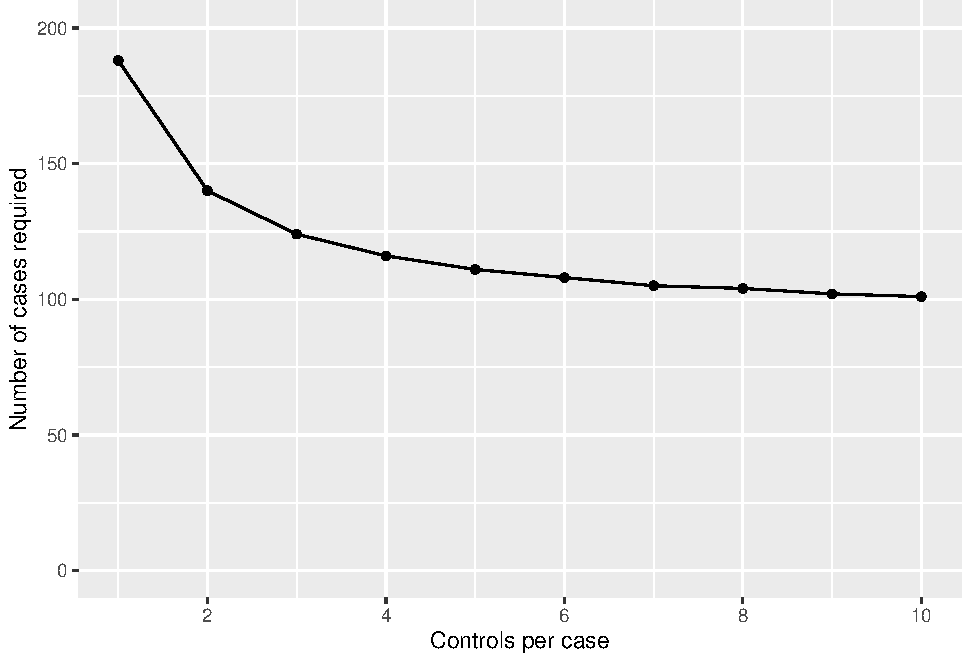
\includegraphics{_main_files/figure-latex/fig-unequal-controls-1.pdf}

We can see that the number of cases required drops off if we go from 1 to 2 controls per case, and again from 2 to 3 controls per case. Once we go from 3 to 4 controls per case, we only reduce the number of cases by 8 (124 vs 116 cases), but at an increase of 91 (371 vs 462) controls. Clearly, this reduction in cases is not offset by the extra controls required.

\hypertarget{limitations-in-sample-size-estimations}{%
\section{Limitations in sample size estimations}\label{limitations-in-sample-size-estimations}}

In this module we have seen how to use Stata for estimating the sample size requirement of a study given the statistical test that will be used and the expected characteristics of the sample. However, once a study is underway, it is not unusual for sample size to be compromised by the lack of research resources, difficulties in recruiting participants or, in a clinical trial, participants wanting to change groups when information about the new experimental treatment rapidly becomes available in the press or on the internet.

One approach that is increasingly being used is to conduct a blinded interim analysis say when 50\% of the total data that are planned have been collected. In this, a statistician external to the research team who is blinded to the interpretation of the group code is asked to measure the effect size in the data with the sole aim of validating the sample size requirement. It is rarely a good idea to use an interim analysis to reduce the planned sample size and terminate a trial early because the larger the sample size, the greater the precision with which the treatment effect is estimated. However, interim analyses are useful for deciding whether the sample size needs to be increased in order to answer the study question and avoid a Type II error.

\hypertarget{summary-1}{%
\section{Summary}\label{summary-1}}

In this module we have discussed the importance of conducting a clinical or epidemiological study with enough participants so that an effect or association can be identified if it exists (i.e.~study power), and how this has to be balanced by the need to not enrol more participants than necessary because of resource issues. We have looked at the parameters that need to be considered when estimating the sample size for different studies and have used a look-up table to estimate required sample size for a prevalence study and Stata to estimate appropriate sample sizes in epidemiological research under the most straightforward situations. The common requirement in all the situations is that the researchers need to specify the minimum effect measure (e.g.~difference in means, OR, RR etc) they want to detect with a given probability (usually 80\% to 90\%) at a certain level of significance (usually P\textless0.05). The ultimate decision on the sample size depends on a compromise among different objectives such as power, minimum effect size, and available resources. To make the final decision, it is helpful to do some trial calculations using revised power and the minimum detectable effect measure.

\hypertarget{module-10-stata-resources}{%
\chapter*{Module 10: Stata resources}\label{module-10-stata-resources}}
\addcontentsline{toc}{chapter}{Module 10: Stata resources}

\hypertarget{learning-activities}{%
\chapter*{\texorpdfstring{\textbf{10} Learning Activities}{10 Learning Activities}}\label{learning-activities}}
\addcontentsline{toc}{chapter}{\textbf{10} Learning Activities}

\hypertarget{activity-10.1}{%
\subsection*{Activity 10.1}\label{activity-10.1}}
\addcontentsline{toc}{subsection}{Activity 10.1}

We are planning a study to measure the prevalence of a relatively rare condition (say approximately 5\%) in children age 0-5 years in a remote community.

\begin{enumerate}
\def\labelenumi{\alph{enumi})}
\tightlist
\item
  What type of study would need to be conducted?
\item
  Use the correct sample size table included in your notes to determine how many children would need to be enrolled for the confidence interval to be

  \begin{enumerate}
  \def\labelenumii{\roman{enumii}.}
  \tightlist
  \item
    2\%
  \item
    4\% around the prevalence?
  \end{enumerate}
\end{enumerate}

What would the resulting prevalence estimates and 95\% CIs be?

\hypertarget{activity-10.2}{%
\subsection*{Activity 10.2}\label{activity-10.2}}
\addcontentsline{toc}{subsection}{Activity 10.2}

We are planning an experimental study to test the use of a new drug to alleviate the symptoms of the common cold compared to the use of Vitamin C. Participants will be randomised to receive the new experimental drug or to receive Vitamin C. How many participants will be required in each group (power = 80\%, level of significance = 5\%).

\begin{enumerate}
\def\labelenumi{\alph{enumi})}
\tightlist
\item
  If the resolution of symptoms is 10\% in the control group and 40\% in the new treatment group?
\item
  How large will the sample size need to be if we decide to recruit two control participants to every intervention group participant?
\item
  If we decide to retain a 1:1 ratio of participants in the intervention and controls groups but the resolution of symptoms is 20\% in the control group and 40\% in the new treatment group?
\item
  How many participants would we need to recruit (calculated in c) if a pilot study shows that 15\% of people find the new treatment unpalatable and therefore do not take it?
\end{enumerate}

\hypertarget{activity-10.3}{%
\subsection*{Activity 10.3}\label{activity-10.3}}
\addcontentsline{toc}{subsection}{Activity 10.3}

In a case-control study, we plan to recruit adult males who have been exposed to fumes from an industrial stack near their home and a sample of population controls in whom we expect that 20\% may also have been exposed to similar fumes through their place of residence or their work.
We want to show that an odds ratio of 2.5 for having respiratory symptoms associated with exposure to fumes is statistically significant.

\begin{enumerate}
\def\labelenumi{\alph{enumi})}
\tightlist
\item
  What statistical test will be needed to measure the association between exposure and outcome?
\item
  How large will the sample size need to be to show that the OR of 2.5 is statistically significant at P \textless{} 0.05 with 90\% power if we want to recruit equal number of cases and controls?
\item
  What would be the required sample size (calculated in b) if the minimum detectable OR were 1.5?
\item
  If there are problems recruiting cases to detect an OR of 1.5 (as calculated in c), what would the sample size need to be if the ratio of cases to controls was increased to 1:3?
\end{enumerate}

\hypertarget{activity-10.4}{%
\subsection*{Activity 10.4}\label{activity-10.4}}
\addcontentsline{toc}{subsection}{Activity 10.4}

In the above study to measure the effects of exposure to fumes from an industrial stack, we also want to know if the stack has an effect on lung function which can be measured as forced vital capacity in 1 minute (FEV1). This measurement is normally distributed in the population.

\begin{enumerate}
\def\labelenumi{\alph{enumi})}
\tightlist
\item
  If the research question is changed to wanting to show that the mean FEV1 in the exposed group is lower than the mean FEV1 in the control group what statistical test will now be required?
\item
  Population statistics show that the mean FEV1 and its SD in the general population for males are 4.40 L (SD=1.25) which can be expected in the control group.
\end{enumerate}

We expect that the mean FEV1 in the cases may be 4.0 L.
How many participants will be needed to show that this mean value is significantly different from the control group with P \textless{} 0.05 with an 80\% power if we want to recruit equal number in each group?

\begin{enumerate}
\def\labelenumi{\alph{enumi})}
\setcounter{enumi}{2}
\tightlist
\item
  How much larger will the sample size need to be if the mean FEV1 in the cases is 4.20 L?
\end{enumerate}

  \bibliography{book.bib,PHCM9795.bib}

\end{document}
